% mnras_template.tex 
%
% LaTeX template for creating an MNRAS paper
%
% v3.0 released 14 May 2015
% (version numbers match those of mnras.cls)
%
% Copyright (C) Royal Astronomical Society 2015
% Authors:
% Keith T. Smith (Royal Astronomical Society)

% Change log
%
% v3.0 May 2015
%    Renamed to match the new package name
%    Version number matches mnras.cls
%    A few minor tweaks to wording
% v1.0 September 2013
%    Beta testing only - never publicly released
%    First version: a simple (ish) template for creating an MNRAS paper

%%%%%%%%%%%%%%%%%%%%%%%%%%%%%%%%%%%%%%%%%%%%%%%%%%
% Basic setup. Most papers should leave these options alone.
\documentclass[fleqn, usenatbib]{mnras}

% MNRAS is set in Times font. If you don't have this installed (most LaTeX
% installations will be fine) or prefer the old Computer Modern fonts, comment
% out the following line
\usepackage{newtxtext,newtxmath}
% Depending on your LaTeX fonts installation, you might get better results with one of these:
%\usepackage{mathptmx}
%\usepackage{txfonts}

% Use vector fonts, so it zooms properly in on-screen viewing software
% Don't change these lines unless you know what you are doing
\usepackage[T1]{fontenc}
\usepackage{ae,aecompl}


%%%%% AUTHORS - PLACE YOUR OWN PACKAGES HERE %%%%%
%\usepackage{caption}
% \usepackage{subcaption}
\usepackage{multirow}
\usepackage{tikz} % to draw neural network
\usepackage{ulem}
% \usepackage{float}
\graphicspath{{figures/}}


% Only include extra packages if you really need them. Common packages are:
\usepackage{graphicx}	% Including figure files
\usepackage{amsmath}	% Advanced maths commands
\usepackage{amssymb}	% Extra maths symbols
\usepackage{enumitem}
% \usepackage[justification=centering]{caption}

%%%%%%%%%%%%%%%%%%%%%%%%%%%%%%%%%%%%%%%%%%%%%%%%%%
\setlist[itemize,1]{leftmargin=\dimexpr 26pt+0.0in}
%%%%% AUTHORS - PLACE YOUR OWN COMMANDS HERE %%%%%
\def\layersep{2.5cm}
\newcommand{\vdag}{(v)^\dagger}
\newcommand\latex{La\TeX}
\newcommand{\hs}[1]{(\textcolor{magenta}{HS:#1})}
\newcommand{\hsd}[1]{\textcolor{magenta}{#1}}
\newcommand{\mro}[1]{\textcolor{red}{\sout{#1}}}
\newcommand{\mrc}[1]{\textcolor{red}{#1}}
\newcommand{\rbd}[1]{\textcolor{blue}{#1}}
\newcommand{\lnHI}{$lnHI$}
%\newcommand{\deg}{{\rm deg}}
% Please keep new commands to a minimum, and use \newcommand not \def to avoid
% overwriting existing commands. Example:
%\newcommand{\pcm}{\,cm$^{-2}$}	% per cm-squared

%%%%%%%%%%%%%%%%%%%%%%%%%%%%%%%%%%%%%%%%%%%%%%%%%%

%%%%%%%%%%%%%%%%%%% TITLE PAGE %%%%%%%%%%%%%%%%%%%

% Title of the paper, and the short title which is used in the headers.
% Keep the title short and informative.
\title[Improving Galaxy Clustering with Deep Learning]{Improving Galaxy Clustering Measurements with Deep Learning: analysis of the DECaLS DR7 data}

% The list of authors, and the short list which is used in the headers.
% If you need two or more lines of authors, add an extra line using \newauthor
\author[M. Rezaie et al.]{
Mehdi Rezaie$^{1}$\thanks{E-mail: mr095415@ohio.edu},
Hee-Jong Seo$^{1}$\thanks{E-mail: seoh@ohio.edu},
Ashley J. Ross$^{2}$,
and Razvan C. Bunescu$^{3}$
\\
% List of institutions
$^{1}$Department of Physics and Astronomy, Ohio University, Athens, OH 45701, USA\\
$^{2}$The Center of Cosmology and Astro Particle Physics, the Ohio State University, Columbus, OH 43210, USA\\
$^{3}$School of Electrical Engineering and Computer Science, Ohio University, Athens, OH 45701, USA
}

% These dates will be filled out by the publisher
\date{Accepted XXX. Received YYY; in original form ZZZ}

% Enter the current year, for the copyright statements etc.
\pubyear{2019}

% Don't change these lines
% \hypersetup{draft} 
\begin{document}
\label{firstpage}
\pagerange{\pageref{firstpage}--\pageref{lastpage}}
\maketitle


\begin{abstract}
Robust measurements of cosmological parameters from galaxy surveys rely on our understanding of systematic effects that impact the observed galaxy density field. In this paper we present, validate, and implement the idea of adopting the systematics mitigation method of Artificial Neural Networks for modeling the relationship between the target galaxy density field and various observational realities including but not limited to Galactic extinction, seeing, and stellar density. Our method by construction does not assume a fitting model a priori and is less prone to over-training by performing k-fold cross-validation and dimensionality reduction via backward feature elimination. By permuting the choice of the training, validation, and test sets, we construct a selection mask for the entire footprint.  We apply our method on the extended Baryon Oscillation Spectroscopic Survey (eBOSS) Emission Line Galaxies (ELGs) selection from the Dark Energy Camera Legacy Survey (DECaLS) DR7 data and show that the spurious large-scale contamination due to imaging systematics can be significantly reduced by up-weighting the observed galaxy density using the selection mask from the neural network and that our method is more effective than the conventional linear and quadratic polynomial functions.  We perform extensive analyses on simulated mock datasets with and without systematic effects. Our analyses indicate that our methodology is more robust to overfitting compared to the conventional methods. This method can be utilized in the catalog generation of future spectroscopic galaxy surveys such as eBOSS and Dark Energy Spectroscopic Instrument (DESI) to better mitigate observational systematics.
\end{abstract}

% 1-6
\begin{keywords}
editorials, notices --- 
miscellaneous --- catalogs --- surveys
\end{keywords}

%
% \tableofcontents 
%
\section{Introduction}\label{sec:intro}
Our current understanding of the Universe is founded upon statistical analyses of cosmological observables, such as the large-scale structure of galaxies, the cosmic microwave background, and the Hubble diagram of distant type Ia supernovae \citep[e.g.,][]{efstathiou1988analysis, fisher1993power, smoot1992structure, mather1994measurement,riess1998observational, perlmutter1999measurements, ata2017clustering, BOSSfinal, jones2018measuring, akrami2018planck, Elvin18}. Among these probes, galaxy surveys aim at constructing clustering statistics of galaxies with which we can investigate the dynamic of the cosmic expansion due to dark energy, test Einstein's theory of gravity, and constrain the total mass of neutrinos and statistical properties of the primordial fluctuations, etc \citep{peebles1973statistical,kaiser1987clustering,mukhanov1992theory,hamilton1998linear,eisenstein1998cosmic,seo2003probing,eisenstein2005dark,sanchez2008best, dalal2008imprints}.\\

The field of cosmology has been substantially advanced by the recent torrents of spectroscopic and imaging datasets from galaxy surveys such as the Sloan Digital Sky Survey (SDSS), Two Degree Field Galaxy Redshift Survey, and WiggleZ Dark Energy Survey \citep{york2000sloan, colless20012df, drinkwater2010wigglez}. The SDSS has been gathering data through different phases SDSS-I (2000-2005), SDSS-II (2005-2008), SDSS-III (2008-2014), and SDSS-IV (2014-2019). In order to derive more robust constraints with higher statistical confidence along with advancements in the technology of spectrographs, software, and computing machines, future large galaxy surveys aim at not only a wider area but also fainter galaxies out to higher redshifts. As an upcoming ground-based survey, the Dark Energy Spectroscopic Instrument (DESI) experiment will gather spectra of thirty million galaxies over 14,000 deg$^{2}$ starting in late 2019; this is approximately a factor of ten increase in the number of galaxy spectra compared to those observed in SDSS I--IV. This massive amount of spectroscopic data will lead to groundbreaking measurements of cosmological parameters through statistical data analyses of the clustering measurements of the 3D distribution of galaxies and quasars \citep{aghamousa2016desi}.\\ 


The Large Synoptic Survey Telescope (LSST) is another ground-based survey currently being constructed. It will gather 20 Terabytes of imaging data every night and will cover 18,000 deg$^{2}$ of the sky for ten years with a sample size of $2\times 10^{9}$ galaxies. The LSST would provide enough imaging data to address many puzzling astrophysical problems from the nature of dark matter, the growth of structure to our own Milky Way. Given such a data volume, many anticipate that the LSST will  revolutionize the way astronomers do research and data analysis \citep{ivezic2008lsst, LSSTObservingStrategyWhitePaper}. \\

The enormous increased data volume provided by DESI and the LSST will significantly improve statistical confidences but will require analyses that are more complex and sensitive to the unknown systematic effects. A particular area of concern is the systematic effects due to imaging attributes such as atmospheric conditions, foreground stellar density, and/or inaccurate calibrations of magnitudes. These systematic effects can affect the target galaxy selections and therefore induce the non-cosmological perturbations into the galaxy density field, leading to excess clustering amplitudes, especially on large scales \citep[see e.g.][]{myers2007clustering,thomas2011angular,thomas2011excess, ross2011ameliorating, ashley2012MNRAS, 2012ApJ...761...14H, huterer2013calibration, pullen2013systematic}.\\ 


Robust and precise measurements of cosmological parameters  from  the large-scale  galaxy  clustering are  contingent  upon  thorough  treatment  of  such  systematic  effects. Many techniques have been developed to mitigate the effects. One can generally classify these  methods  into  the mode projection, regression,  and Monte Carlo simulation of fake objects.\\ 

The mode-projection based techniques attribute a large variance to the spatial modes that strongly correlate with the potential systematic maps such as imaging attributes, thereby effectively removing those modes from the estimation of power spectrum \citep[see e.g.][]{rybicki1992interpolation,tegmark1997measure,tegmark1998measuring,slosar2004exact,ho2008correlation, pullen2013systematic,leistedt2013estimating,leistedt2014exploiting}. In detail, the basic mode projection \citep{leistedt2013estimating} produces an unbiased power spectrum and is equivalent to a marginalization over a free amplitude for the contamination produced by a given map.
 The caveat is that the variance of the estimated clustering increases by projecting out more modes for more imaging attributes. The \textit{extended} mode projection technique \citep{leistedt2014exploiting} resolves this issue by selecting a subset of the imaging maps using a $\chi^{2}$ threshold to determine the significance of a potential map. The limitation of the mode-projection based methods is that they are only applicable to the two-dimensional clustering measurements, and they reintroduce a small bias \citep{elsner2015unbiased}. \citet{kalus2016unbiased} extended the idea to the 3D clustering statistics and developed a new step to unbias the measurements~\citep[for an application on SDSS-III BOSS data see e.g.,][]{kalus2018map}\\

The regression based techniques model the dependency of the galaxy density on the potential systematic fluctuations and estimate the parameters of the proposed function by solving a least-square problem, or by cross correlating the galaxy density map with the potential systematic maps \citep[see e.g.][]{ross2011ameliorating, ashley2012MNRAS,Ross17,2012ApJ...761...14H,delubac2016sdss, prakash2016sdss, Raichoor2017MNRAS.471.3955R, laurent2017clustering, Elvin18}. The best fit model produces a \textit{selection mask (function)} or a set of \textit{photometric weights} that quantifies the systematic effects in the galaxy density fluctuation induced by the imaging pipeline, survey depth, and other observational attributes. The selection mask is then used to up-weight the observed galaxy density map to mitigate the systematic effects. The regression-based methods often assume a linear model (with linear or quadratic polynomial terms), and use all of the data to estimate the parameters of the given regression model; however, the assumption that the systematic effects are linear might not necessarily hold for strong contamination, e.g., close to the Galactic plane. \citet{2012ApJ...761...14H} analyzed photometric Luminous Red Galaxies in SDSS-III Data Release 8 and showed that the excess clustering due to the stellar contamination on large scales (e.g., roughly greater than twenty degrees) cannot be removed with a linear approximation. \citet{rossfNL} investigated the local non-Gaussianity ($f_{NL}$) using BOSS Data Release 9 ``CMASS" sample of galaxies \citep{ahn2012ninth} and found that a robust cosmological measurement on very large scales is essentially limited by the systematic effects. Their analysis indicated that a more effective systematics correction is preferred relative to the selection mask based on the linear modeling of the stellar density contamination. Recently, \citet{Elvin18} developed a methodology based on $\chi^{2}$ statistics to rank the imaging maps based on their significance, and derived the selection mask by regressing against the significant maps.\\

Another promising, yet computationally expensive, approach injects artificial sources into real imaging in order to forward-model the galaxy survey selection mask introduced by real imaging systematics \citep[see e.g.][]{berge2013ultra,Balrog}. Rapid developments of multi-core processors and efficient compilers will pave the path for the application of these methods on big galaxy surveys.\\




In this paper, we develop a systematics mitigation method based on artificial neural networks. Our methodology models the galaxy density dependence on observational imaging attributes to construct the selection mask, without making any prior assumption of the fitting model. Most importantly, this methodology is less prone to over-training and the resulting removal of the clustering signal by performing $k$-fold cross-validation (i.e., splitting the data into $k$ number of groups/partitions from which one constructs the training, validation, and the test sets) and dimensionality reduction through backward feature elimination~(i.e., removing redundant and irrelevant imaging attributes)\citep[see e.g.,][]{devijver1982pattern, john1994irrelevant, koller1996toward, kohavi1997wrappers, ramaswamy2001multiclass, guyon2003introduction}.  By permutation of the training, validation, and test sets, the selection mask for the entire footprint is constructed.  We apply our method on galaxies in the DECaLS DR7 data~\citep{dey2018overview} that are chosen with the eBOSS-ELG selection criteria~\citep{Raichoor2017MNRAS.471.3955R} and compare its performance with that of the conventional, linear and quadratic polynomial regression methods. While the effect of mitigation on the data will be estimated qualitatively as well as quantitatively in reference to the clustering expected based on the concordance $\Lambda$CDM cosmology, the data does not allow an absolute comparison to the unknown truth. We therefore simulate two sets of 100 mock datasets, without and with the systematic effects that mimic those of the real DECaLS DR7 data, apply various mitigation techniques in the same way we treat the real data, and test the resulting clustering signals against the ground truth.\\


This paper is organized as follows. Section \ref{sec:data} presents the imaging dataset from DECaLS DR7 used for our analysis. In Section \ref{sec:method}, we describe our method of Artificial Feed Forward Neural Network in detail as well as the conventional multivariate regression approaches. In this section, we also explain the angular clustering statistics employed to assess the level of systematic effects and the mitigation efficiency. We further describe the procedure of producing the survey mocks with and without simulated contaminations. In Section \ref{sec:results}, we present the results of mitigation for both the DECaLS DR7 dataset and the mocks. Finally, we conclude with a summary of our findings and a discussion of the benefits of our methodology for future galaxy surveys in Section \ref{sec:conclusion}.\\

\section{Legacy Surveys DR7}\label{sec:data}
We use the seventh release of data from the Legacy Surveys \citep{dey2018overview}. The Legacy Surveys are a group of imaging surveys in three optical (r, g, z) and four Wide-field Infrared Survey Explorer (W1, W2, W3, W4; \citet{wright2010wide}) passbands that will provide an inference model catalog amassing 14,000 deg$^{2}$ of the sky in order to pre-select the targets for the DESI survey \citep{lang2016tractor, aghamousa2016desi}. Identification and mitigation of the systematic effects in the selection of galaxy samples from  this imaging dataset is of vital importance to DESI, as spurious fluctuations in the target density will likely present as fluctuations in the transverse modes of the 3D field and/or changes in the shape of the redshift distribution. Both effects will need to be modeled in order to isolate the cosmological clustering of DESI galaxies. The ground-based surveys that probe the sky in the optical bands are the Beijing-Arizona Sky Survey (BASS) \citep{zou2017project}, DECam Legacy Survey (DECaLS) and Mayall z-band Legacy Survey (MzLS)\citep[see e.g.,][]{dey2018overview}. Additionally, the Legacy Surveys program takes advantage of another imaging survey, the Dark Energy Survey, for about 1,130 deg$^{2}$ of their southern sky footprint \citep{dark2005dark}. \\

We consider a total of 18 imaging attributes as potential sources of the systematic error since each of these attributes can affect the completeness and purity with which galaxies can be detected in the imaging data. We produce the HEALPIX maps \citep{gorski2005healpix} for these attributes based on the DR7 ccds-annotated file using the \texttt{validationtests} pipeline\footnote{\url{https://github.com/legacysurvey/legacypipe/tree/master/validationtests}} and the code that uses the methods described in \citet{LeistedtMap}. We use the resolution of $nside=256$, \textit{ring} ordering scheme, and oversampling of four\footnote{In this context, `oversampling' means dividing a pixel into sub-pixels in order to derive the given pixelized quantity more accurately. For example, oversampling of four means subdividing each pixel into $4^2$ sub-pixels. If the target resolution is nside=256, the attributes will be derived based on a map with resolution of 4$\times$256 when oversampling is four.}. These include three maps of Galactic structure: Galactic extinction \citep{schlegel1998maps}, stellar density from Gaia DR2 \citep{brown2018gaia}, and Galactic neutral atomic hydrogen (HI) column density \citep{bekhti2016hi4pi}. We further pixelize quantities associated with the Legacy Surveys observations, including the total depth, mean seeing, mean sky brightness, minimum modified Julian date, and total exposure time in three passbands (r, g, and z).  For clarity, we list each attribute below:\\

\begin{itemize}
    \item \textbf{Galactic extinction} (\textit{EBV}), measured in magnitudes, is the infrared radiation of the dust particles in the Milky Way \footnote{The dust particles in the Galactic plane absorb and scatter the optical light in the infrared.} which affects the brightness of the objects, i.e., the detectability of the targets. We correct the magnitudes of the objects for the Milky Way extinction prior to the galaxy (\textit{target}) selection.\\
    
    \item \textbf{Galaxy depth} (\textit{depth}) defines the brightness of the faintest detectable galaxy at $5-\sigma$ confidence, measured in AB magnitudes. Since the depth and extinction (EBV) are somewhat related, we correct the depth magnitudes for the extinction effect, with the extinction coefficients of 2.165, 3.214 and 1.211 respectively for r, g and z bands \citep{schlafly2011measuring}.\\
    
    \item {\bf Stellar density} (\textit{nstar}), measured in deg$^{-2}$, is constructed by pixelization of the Gaia DR2 star catalog \citep{brown2018gaia} with the g-magnitude cut of 12 < gmag < 17. The stellar foreground affects the galaxy density in two ways. First, stars can be mis-identified as galaxies and included in the sample, which will result in a positive correlation between the stellar and galaxy distribution. Second, the foreground light from stars impacts the ability to detect the galaxies that are behind them, e.g., by directly obscuring their light or by altering the sky background, which will cause a negative correlation between the two distributions. The second effect may reduce the completeness with which galaxies are selected and was the dominant systematic effect on the BOSS galaxies \citep{ashley2012MNRAS}. \\
    
    \item \textbf{Hydrogen atom column density} (\textit{HI}), measured in cm$^{-2}$, is another useful tracer of the Galactic structure, which increases at regions closer to the Milky Way plane. This map provides complementary information to the Galactic extinction and stellar density maps. Hereafter, \text{\lnHI} refers to the natural logarithm of the HI column density.\\

  {\bf Sky brightness} (\textit{skymag}) relates to the background level that is estimated and subtracted from the images as part of the photometric processing. It thus alters the depth of the imaging. It is measured in AB mag/arcsec$^{2}$. \\


    \item {\bf Seeing} (\textit{seeing}) is the full width at half maximum of the point spread function (PSF), i.e., the sharpness of a telescope image, measured in arc seconds. It quantifies the turbulence in the atmosphere at the time of the observation, and is sensitive to the optical system of the telescope, e.g., whether or not it is out of focus. Bad seeing conditions can make stars that are point sources appear as extended objects, therefore falsely being selected as galaxies. We use a multiplicative factor of 0.262 to transform the seeing unit from ccd `pixel' to arc seconds.\\

    \item {\bf Modified Julian Date} (\textit{MJD}) is the traditional dating method used by astronomers, measured in days. If a portion of data taken during a specific period is affected by observational conditions during that period, regressing against MJD could mitigate that effect.\\

    \item {\bf Exposure time} (\textit{exptime}) is the length of time, measured in seconds, during which the ccd was exposed to the object light. Longer exposures are needed to observe fainter objects. The Legacy Surveys data is built up from many overlapping images, and we map the total exposure time, per band, in any given area. A longer exposure time thus corresponds to a greater depth, all else being equal.
\end{itemize}

As part of the process of producing the maps, we determine the fractional ccd coverage per passband, fracgood ($f_{{\rm pix}}$), within each pixel with oversampling of four. We take the minimum of $f_{{\rm pix}}$ in r, g, and z passbands as the \textit{completeness} weight of each pixel. We apply the following arbitrary cuts, somewhat motivated by the eBOSS selection, on the depth and $f_{{\rm pix}}$ values: \\
\begin{align}\label{eq:depth_cuts}
depth_{r} &\geq 22.0, \\
depth_{g} &\geq 21.4, \nonumber\\
depth_{z} &\geq 20.5, \nonumber\\
{\rm and}~f_{\rm pix}  &\geq 0.2, \nonumber
\end{align}
which results in 187257 pixels and an effective total area of 9,459 $\deg^2$ after taking $f_{{\rm pix}}$ into account. We report the mean and standard deviation of the imaging attributes on the masked footprint in Tab. \ref{tab:meanstats}.\\

\begin{table}
	\centering
	\caption{The mean and sample standard deviation of the DECaLS DR7 imaging attributes used in this paper.}
	\label{tab:meanstats}
	\begin{tabular}{lcr} % four columns, alignment for each
	    \hline
		\hline
		Imaging map & mean & standard deviation \\
		\hline
         EBV [mag] & 4.8480e-02 & 3.1917e-02 \\ 
        ln(HI/cm$^{2}$) & 4.7211e+01 & 4.8513e-01 \\ 
        nstar [deg$^{-2}$] & 8.4525e+02 & 6.3729e+02 \\ 
        \hline
        depth-r [mag] & 2.3960e+01 & 1.4257e+00 \\ 
        depth-g [mag] & 2.4339e+01 & 1.2023e+00 \\ 
        depth-z [mag] & 2.2927e+01 & 7.9275e-01 \\ 
        \hline
        seeing-r [arcsec] & 1.4089e+00 & 2.6377e-01 \\ 
        seeing-g [arcsec]& 1.5561e+00 & 2.7077e-01 \\ 
        seeing-z [arcsec]& 1.3128e+00 & 2.2542e-01 \\ 
        \hline
        skymag-r [mag/arcsec$^{2}$] & 2.3957e+01 & 6.1772e-01 \\ 
        skymag-g [mag/arcsec$^{2}$] & 2.5394e+01 & 5.0522e-01 \\ 
        skymag-z [mag/arcsec$^{2}$]& 2.2041e+01 & 4.2714e-01 \\ 
        \hline
        exptime-r [sec] & 4.8068e+02 & 2.0174e+03 \\ 
        exptime-g [sec]& 6.8061e+02 & 2.4920e+03 \\ 
        exptime-z [sec]& 6.5157e+02 & 5.2295e+03 \\
        \hline
        mjd-r [day] & 5.7233e+04 & 5.5595e+02 \\ 
        mjd-g [day] & 5.7358e+04 & 5.1123e+02 \\ 
        mjd-z [day] & 5.7005e+04 & 4.3704e+02 \\ 
		\hline
		\hline
	\end{tabular}
\end{table}
 
 
\begin{table}
  \begin{center}
    \caption{The Northern Galactic Cap color-magnitude selection of the eBOSS Emission Line Galaxies \citep{Raichoor2017MNRAS.471.3955R}. We enforce the same selection for the entire sky. Note that our selection is slightly different from \citet{Raichoor2017MNRAS.471.3955R} in the clean photometry criteria as explained in the main text.}
    \label{tab:ts}
    \begin{tabular}{l|r}
    \hline
	\hline
      \textbf{Criterion} & \textbf{eBOSS ELG}\\
      \hline
      \multirow{4}{*}{\scriptsize{Clean Photometry}} & \scriptsize{0 mag $<$ V $<$ 11.5 mag Tycho2 stars mask}\\
& \scriptsize{\texttt{BRICK\_PRIMARY}==True}\\
& \scriptsize{\texttt{brightstarinblob}==False} \\~\\
      \scriptsize{[OII] emitters} &  \scriptsize{21.825 $<$ g $<$ 22.9} \\~\\
      \multirow{2}{*}{\scriptsize{Redshift range}} & \scriptsize{-0.068(r-z) + 0.457 $<$ g-r $<$ 0.112 (r-z) + 0.773}\\
 & \scriptsize{0.637(g-r) + 0.399 $<$ r-z $<$ -0.555 (g-r) + 1.901}\\
      \hline
      \hline
      \end{tabular}
  \end{center}
\end{table}


To construct the ELG catalog, we enforce the Northern Galactic Cap eBOSS ELG selection color-magnitude criteria from \citet{Raichoor2017MNRAS.471.3955R} on DR7 sweep files \citep{dey2018overview} with a few differences in the clean photometry criteria (see Table \ref{tab:ts}). In detail, the original eBOSS ELG selection is based on DR3 while ours is based on DR7. Since the data structure changed from DR3 to DR7, we use \texttt{brightstarinblob} instead of \texttt{tycho2inblob} to eliminate objects that are near bright stars. In contrast to the original selection criteria, we do not apply the \texttt{decam\_anymask[grz]=0} cut, as any effect from this cut will be encapsulated by the 18 imaging attribute maps we employ. Also, we drop the SDSS bright star mask from the criteria, as this mask is essentially replaced by the \texttt{brightstarinblob} mask. After constructing the galaxy catalog, we pixelize the galaxies into a Healpix map with \textit{nside} of 256 in ring ordering format to create the observed galaxy density map.\\


\begin{figure*}
    \centering
    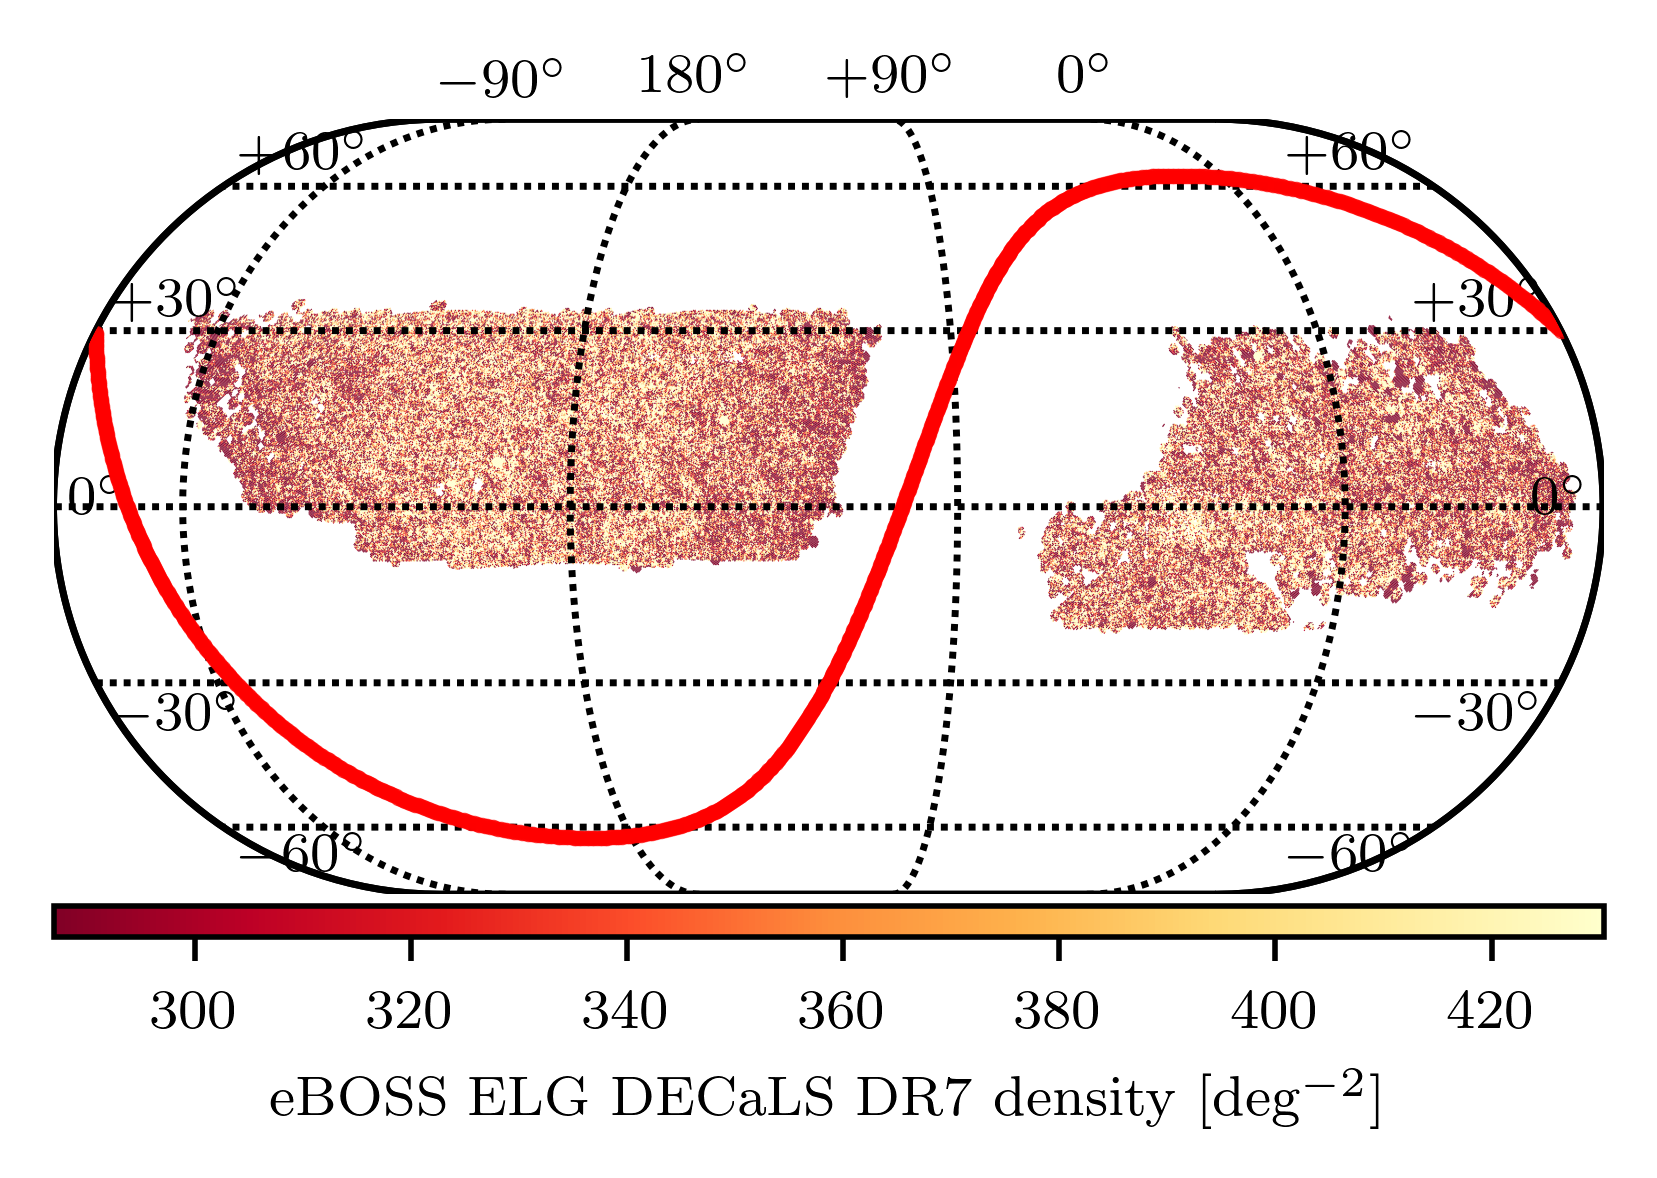
\includegraphics[width=0.65\textwidth]{eboss-dr7.png}
    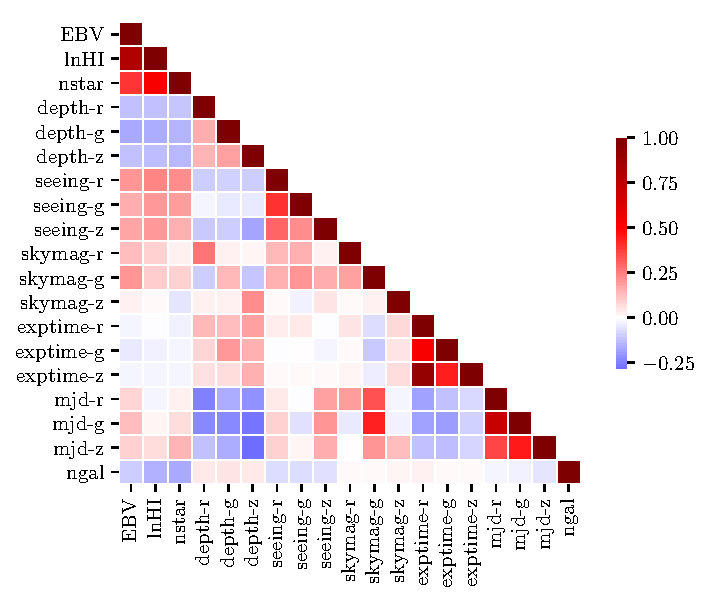
\includegraphics[width=0.65\textwidth]{corrmax-dr7.pdf}
    \caption{\textit{Top panel}: the pixelated density map of eBOSS-like ELGs from the DECaLS DR7 after correcting for the completeness of each pixel and masking based on the survey depth and completeness cuts. The solid red curve represents the Galactic plane. This figure is generated by the code described in \url{https://nbviewer.jupyter.org/github/desihub/desiutil/blob/master/doc/nb/SkyMapExamples.ipynb}. \textit{Bottom panel}: the color-coded Pearson correlation matrix between each pair of the imaging attributes from the DECaLS DR7.}
    \label{fig:eboss_dr7}
\end{figure*}


As an exploratory analysis, we use the Pearson correlation coefficient (PCC) to assess the linear correlation between the data attributes. For two variables $X$ and $Y$, PCC is defined as,
\begin{equation}\label{eq:pcc}
\rho_{X, Y} = \frac{cov(X, Y)}{\sqrt{cov(X,X)cov(Y,Y)}},
\end{equation}
where $cov(X,Y)$ is the covariance between $X$ and $Y$ across all pixels. In Fig.~\ref{fig:eboss_dr7}, we show the observed galaxy density after the pixel completeness (i.e., fracgood $f_{\rm pix}$) correction in the top panel and the correlation (PCC) matrix between the DR7 attributes as well as the galaxy density (\textit{ngal}, the bottom row) in the bottom panel. These statistics indicate that Galactic foregrounds, such as stellar density $nstar$, neural hydrogen column density \lnHI, and Galactic extinction $EBV$, are moderately anti-correlated with the observed galaxy density. Each of these maps traces the structure of the Milky Way and the anti-correlation with $ngal$ implies that, for example, closer to the Galactic plane where the extinction and stellar density are high, there is a systematic decline in the density of galaxies we selected in our sample. The top-left corner of Fig.~\ref{fig:eboss_dr7} shows that these three imaging attributes are strongly correlated with each other. Likewise, the negative correlation of $ngal$ with $seeing$ indicates that as $seeing$ increases the detection of ELGs becomes more challenging. On the other hand, we find a positive correlation between $ngal$ and $depth$s, which can be explained by the fact that as the depth decreases, e.g., we cannot observe fainter objects, the number of galaxies decreases as well.\\

This matrix overall demonstrates that the correlation among the imaging variables is not negligible. For instance, in addition to the correlation among the Galactic Foreground attributes aforementioned, there is an anti-correlation between the MJD and depth values. Likewise, there is an anti-correlation between the seeing and depth values. The complex correlation between the imaging attributes means that such correlations should be all taken into account when modeling the galaxy density dependence on the imaging attributes.

\section{Methodology}\label{sec:method}

\subsection{Observed galaxy density}
In our methodology, we treat the mitigation of imaging systematics as a regression problem, in which we aim to model the relationship between the observed galaxy density (\textit{label}) and the imaging attributes (\textit{features}) that are the potential sources of the systematic error. Note that we do not include the positional information as \textit{input} features since we do not want the mitigation to fit to the cosmological clustering pattern. The solution of the regression then would provide the predicted mean galaxy density (i.e., in the absence of clustering or shot-noise) solely based on the imaging attributes of that location. We use this predicted galaxy density as the \textit{survey} selection mask to be applied to any observed galaxy map in the attempt to eliminate the systematic effects and therefore isolate the cosmological fluctuation. Below we describe our procedure.\\


The observed number of galaxies within pixel $i$ can be expressed in terms of the true number of galaxies $n_{i}$ and the contamination model $\mathcal{F}(\textbf{s}_{i})$ as 
\begin{equation}\label{eq:ngal_fs}
    n_{i}^{o}(\textbf{s}_{i}) = n_{i} \mathcal{F}(\textbf{s}_{i}), 
\end{equation}
where \textbf{s}$_{i}$ is a vector representing the imaging attributes of pixel $i$, and the contamination model $\mathcal{F}(\textbf{s}_i)$ is an unknown function representing the systematic effects which could be either a linear, non-linear, or a more complex combination of the imaging attributes. The modeling of $\mathcal{F}(\textbf{s}_{i})$ can be approached by a wide variety of techniques, ranging from the traditional methods based on multivariate functions to non-parametric and non-linear models based on machine learning or deep learning such as random tree forests and neural networks \citep{breiman2001random, geurts2006extremely}.\\

The cosmological information is contained in the true overdensity that is given by
\begin{equation}
\delta_{i} = n_i/(f_{{\rm pix},i}\bar{n})-1,\label{eq:overden}
\end{equation}
accounting for the pixel completeness where $\bar{n}$ is the `true' average number of galaxies. Then,
\begin{equation}
n_{i}^{o}= f_{{\rm pix},i}\overline{n}~(1 + \delta_{i})~ \mathcal{F}(\textbf{s}_{i}).\label{eq:nobsi}
\end{equation}
This $n_{i}^{o}/f_{{\rm pix},i}$ is equivalent to the observed $ngal$ aforementioned.
Since we do not know the true average number density $\overline{n}$ of the data, we estimate $\bar{n}$ from the average of the observed galaxy field,
\begin{equation}\label{eq:nbar}
\hat{\overline{n}} = \frac{\displaystyle\sum_{i} n^{o}_{i}  }{\displaystyle\sum_{i} f_{{\rm pix},i}},
\end{equation}
and treat $\hat{\overline{n}} \equiv \overline{n}$.
Due to the finite volume of our sample, $\hat{\overline{n}} \neq \overline{n}$ even in the absence of systematic effects. This imposes the well-known integral constraint effect on any clustering analysis. We further ignore any systematic effect on $\hat{\overline{n}}$ due to the fact we use $n^{o}_{i}$; that is, Eq.~\ref{eq:nbar} converges to $\overline{n}$ only when $\sum_{i} f_{{\rm pix},i}= \sum_{i} f_{{\rm pix},i}\mathcal{F}_i$. 
In this sense we are modeling the relative systematic effect without necessarily determining the accurate `true' $\overline{n}$. We will use simulated results to test our methodology, and the analysis applied to the simulations with a limited footprint will be subject to the similar finite-volume and systematic effects on $\hat{\overline{n}}$, thus providing a fair comparison and means to catch any obvious problem with this approximation.\\

Finally, we define the normalized galaxy density per pixel $t_{i}$,
\begin{equation}\label{eq:nnbar}
    t_{i}(\textbf{s}_{i}) \equiv \frac{n_{i}^{o}(\textbf{s}_{i})}{f_{{\rm pix},i}\hat{\overline{n}}} = (1+\delta_{i}) ~ \mathcal{F}(\textbf{s}_{i}).
\end{equation}
With this definition, we can estimate the unknown contamination model $\hat{\mathcal{F}}$ (or selection mask) by modeling the dependence of $t$ on \textbf{s}. When averaged over many spatial positions, the cosmological fluctuations $\delta_i$ will be averaged out and therefore the observed $t_i$ averaged across many pixels with the same \textbf{s} should only be a function of $\textbf{s}$ and return $\mathcal{F}(\textbf{s})$:
\begin{equation}\label{eq:tfs}
    <t_{i}(\textbf{s})>_i  \simeq {\mathcal{F}}(\textbf{s}).
\end{equation}
The inverse of the selection mask which is equivalent to the photometric weights ($wt^{{\rm sys}}$) in other studies can therefore be used to remove the systematic effects from the observed galaxy number map (cf. Eq. \ref{eq:ngal_fs}),

\begin{align}\label{eq:wsys}
\hat{n}_i = \frac{n^o_i}{\hat{\mathcal{F}}}=n^o_i wt^{{\rm sys}}_{i}.
\end{align}
In the following we describe how we obtain $\hat{\mathcal{F}}$ using different regression approaches, e.g., neural networks and multivariate linear functions. From now on, the terms \textit{features} and \textit{label} associated with each data point refer to \textbf{s} and $t$ of each HEALPIX pixel, respectively. 

\subsection{Mitigation with Neural Networks}\label{subsec:MethodNN}
We will apply {\it fully connected feed forward neural networks} in order to tackle our regression problem. Fig. \ref{fig:perceptron} illustrates a schematic diagram of a neuron, the building block of a neural network, which generates the output based on a linear combination of the inputs followed by a nonlinear transformation, the activation function $f$.\\

\begin{figure}
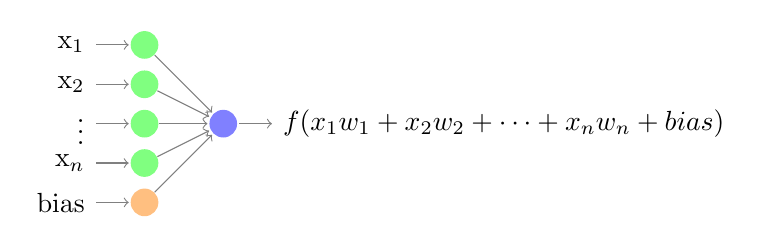
\begin{tikzpicture}[shorten >=0.5pt,->,draw=black!50, node distance=1.cm]
    \tikzstyle{every pin edge}=[<-,shorten <=0.5pt]
    \tikzstyle{neuron}=[circle,fill=black!25,minimum size=10pt,inner sep=0pt]
    \tikzstyle{input neuron}=[neuron, fill=green!50];
    \tikzstyle{hidden neuron}=[neuron, fill=blue!50];
    \tikzstyle{bias neuron}=[neuron, fill=orange!50];
    % Draw the input layer nodes
    \foreach \name / \y in {x$_{1}$/3, x$_{2}$/4, \vdots/5, x$_{n}$/6}
        \node[input neuron, pin=left:\name] (I-\y) at (1. cm,-0.5*\y cm) {};            
    \node[bias neuron, pin=left:bias] (I-7) at (1. cm,-3.5) {};          
     % Draw the output layer node
    \node[hidden neuron,pin={[pin edge={->}]right:$f(x_{1}w_{1} + x_{2}w_{2}+ \cdots + x_{n}w_{n}+ bias)$}, right of=I-5] (O) {};
    \foreach \source in {3,...,7}
        \path (I-\source) edge (O);
\end{tikzpicture}
\caption{A schematic diagram of a single neuron with the activation function $f$. The neuron takes a set of inputs \textbf{x}=$(x_{1}, x_{2},...,x_{n})$, multiplies each of them by its associated weight \textbf{w}=$(w_{1}, w_{2},...,w_{n})$, and sums the weighted values and a thresh-hold (or a constant offset) which is called \textit{bias}, to form a pre-activation value, $z=\sum_{i=1}^{n}x_{i}w_{i} + bias$, which is a linear process. The neuron then transforms the pre-activation $z$ to the output using the activation function $f(z)$, which is where the nonlinear process can enter. }\label{fig:perceptron}
\end{figure}

Fig. \ref{fig:ffnn} illustrates the architecture of a fully connected feed forward neural network with the imaging attributes in the input layer, three hidden layers of six non-linear neurons in the middle, and a single neuron without any activation function in the output layer, as an example. The \textit{bias} neuron in each layer is shown in orange and is analogous to the intercept in linear regression. The output of the neural network will be an estimation of the contamination model $\hat{\mathcal{F}}$ (see Eq. \ref{eq:nnbar}). If we use the identity function as the activation function (e.g., $f(z)=z$), regardless of the number of hidden layers, the neural network is equivalent to a linear model. This means that our methodology is a generalization or an extension of the conventional linear mitigation methods. The modeling capabilities of neural networks depend on the number of hidden layers, type of non-linear activation function and the number of neurons in each hidden layer \citep[see e.g.][]{cybenko1989approximation,hornik1989multilayer,funahashi1989approximate, tamura1997capabilities, huang2003learning, lin2017does, rolnick2017power}.\\

We use the rectifier $f(z) = \text{max}(0, z)$ as the activation function for the hidden layer neurons, which alleviates the `vanishing gradient' problem
~\citep[see e.g.,][]{nair2010rectified,glorot2011deep,krizhevsky2012imagenet, dahl2013improving,montufar2014number}. \\

\begin{figure}
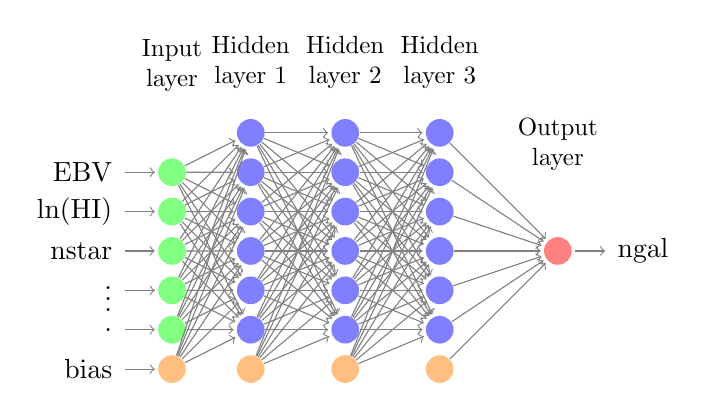
\begin{tikzpicture}[shorten >=1pt,->,draw=black!50, node distance=1.5cm]
    \tikzstyle{every pin edge}=[<-,shorten <=1pt]
    \tikzstyle{neuron}=[circle,fill=black!25,minimum size=10pt,inner sep=0pt]
    \tikzstyle{input neuron}=[neuron, fill=green!50];
    \tikzstyle{output neuron}=[neuron, fill=red!50];
    \tikzstyle{hidden neuron}=[neuron, fill=blue!50];
    \tikzstyle{bias neuron}=[neuron, fill=orange!50];
    \tikzstyle{annot} = [text width=4em, text centered, scale=0.9]
    % Draw the input layer nodes
    \foreach \name / \y in {EBV/1, ln(HI)/2, nstar/3, \vdots/4, ./5}
        \node[input neuron, pin=left:\name] (I-\y) at (0,-0.5*\y) {};
    \node[bias neuron, pin=left:bias] (I-6) at (0,-3.) {};         
    % Draw first hidden layer nodes
    \foreach \name / \y in {1,...,6}
        \path[yshift=0.5cm]
            node[hidden neuron] (H-\name) at (1.0 cm,-0.5*\y cm) {}
            node[hidden neuron] (G-\name) at (2.2 cm,-0.5*\y cm) {}    
            node[hidden neuron] (L-\name) at (3.4 cm,-0.5*\y cm) {};                        
    \node[bias neuron] (H-7) at (1.0 cm,-3. cm) {};
    \node[bias neuron] (G-7) at (2.2 cm,-3. cm) {};            
    \node[bias neuron] (L-7) at (3.4 cm,-3. cm) {};
     % Draw the output layer node
    \node[output neuron,pin={[pin edge={->}]right:ngal}, right of=L-4] (O) {};
    % connect nodes
    \foreach \source in {1,...,6}
        \foreach \dest in {1,...,6}
            \path (I-\source) edge (H-\dest);
    \foreach \source in {1,...,7}
        \foreach \dest in {1,...,6}
            \path (H-\source) edge (G-\dest);
    \foreach \source in {1,...,7}
        \foreach \dest in {1,...,6}
            \path (G-\source) edge (L-\dest);
     % Connect every node in the hidden layer with the output layer
    \foreach \source in {1,...,7}
        \path (L-\source) edge (O);
     % Annotate the layers
    \node[annot,above of=I-1] {Input layer};
    \node[annot,above of=H-1, node distance=1.0 cm] (hl1) {Hidden layer 1};
    \node[annot, above of=G-1, node distance=1.0 cm] (hl2) {Hidden layer 2};
    \node[annot, above of=L-1, node distance= 1.0 cm] (hl3){Hidden layer 3};
    \node[annot,above of=O] {Output layer};    
\end{tikzpicture}
\caption{A schematic illustration of a fully connected feed forward neural network with the imaging attributes in the input layer, three hidden layers of six neurons in the middle, and a single neuron on the output layer, as an example. The blue colored neurons have non-linear activation functions, while the red colored neuron lacks any activation function. In reality, we employ the validation procedure to choose the best number of hidden layers while keeping the total number of hidden layer neurons fixed at 40 (i.e., approximately twice the number of imaging attributes in this study).}\label{fig:ffnn}
\end{figure}

We utilize  $k$-fold cross-validation with $k=5$ folds/sub-groups to train the parameters, tune the hyper-parameters, and to estimate the predictive performance of the neural network. As illustrated in Fig. \ref{fig:5fold}, we randomly split the entire pixel data (187257 pixels) into five folds and construct the training, validation and test data sets out of these five folds; three folds are assigned to the training set, one fold is assigned to the validation set, and the remaining one fold is assigned to the test set. A specific assignment of the five folds to these three sets forms one `partition'. We construct five different partitions such that each fold is used once as test fold. This $k$-fold cross-validation scheme ensures that a test example is never used for training or tuning.\\

\begin{figure}
         \centering
         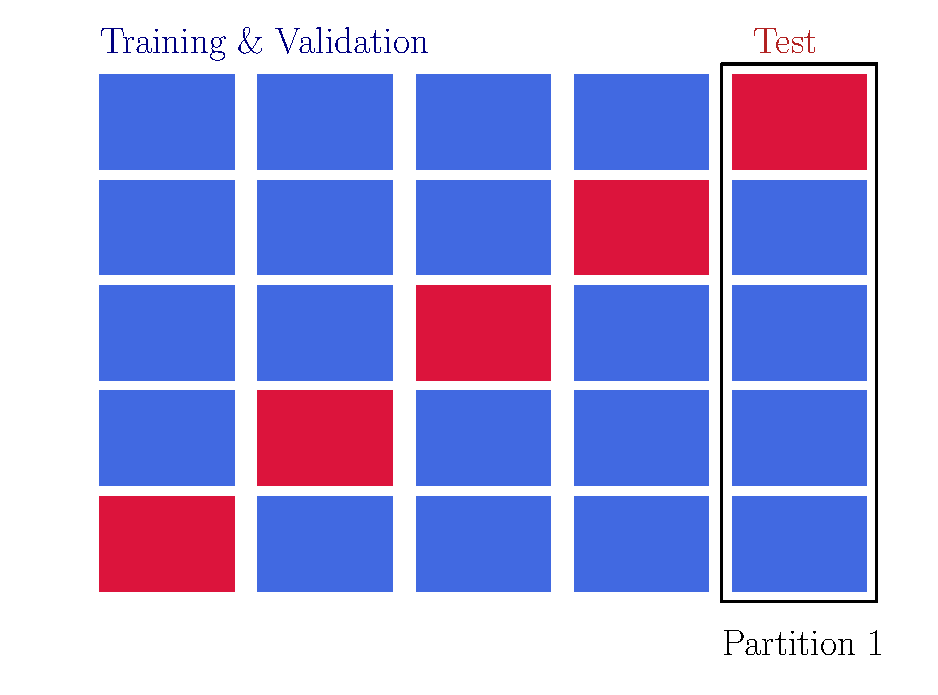
\includegraphics[width=0.4\textwidth]{5folds.pdf}
         \caption{A visualization of the five-fold permutations of data-split. The data is randomly split into five equal-size folds, and by permutation of the folds we construct five partitions of data. For each partition/permutation, three folds are assigned to the training set, one fold for the validation set, and the remaining one fold for the test set: therefore, 60\% training, 20\% validation, and 20\% test sets. Each column represents a partition. The test folds are shown in red, while the training and validation folds are shown in blue. The key points are : 1) The folds are not contiguous (in RA, DEC) as may be implied by this cartoon. 2) There is no overlap between the training, validation, and test folds within a partition. 3) One can reconstruct the entire data by merging the test folds from the five partitions.}
         \label{fig:5fold}
     \end{figure}
     
     
We standardize (i.e., renormalize) the label and features of the training, validation, and test folds using the mean and standard deviation of the label and features of the corresponding training fold (i.e., similar to Tab.~\ref{tab:meanstats}, but for the training set of each partition). We initialize the biases to zero, and sample the weights of each layer randomly from a normal distribution whose variance is inversely proportional to the number of neurons of the previous layer \citep[see e.g.,][]{he2015delving}. Using the training fold, we utilize the adaptive gradient descent with momentum \citep[\textit{Adam},][]{kingma2014adam} to update the parameters of the neural network with batches of size $N_{{\rm batch}}$. Thus, the entire training set is split into $N_{{\rm batch}}$ batches and a gradient update is applied for each batch. One training epoch corresponds to processing the $N_{{\rm batch}}$ batches once \citep[for more details on the training procedure, we refer the reader to see e.g.,][]{ruder2016overview}. The hyper-parameters of \textit{Adam}, specifically the moments decay rates and the tolerance, are fixed as follows: $\beta_{1}$ = 0.9, $\beta_{2}$ = 0.999 and $\epsilon$ = 10$^{-8}$. The default learning rate of 0.001 will be tuned using the validation data.\\ 

The network is trained to minimize the following cost function:
\begin{equation}\label{eq:cost}
    \text{J} = \frac{1}{N_{{\rm batch}}}\sum_{i}^{N_{{\rm batch}}}f_{\rm pix, i}~[t_{i} - \hat{\mathcal{F}_{i}}]^{2} + \frac{\lambda}{2} ~ ||w||^{2} ,
\end{equation}   
%
where the first term is the Mean Squared Error (MSE) weighted with $f_{\rm pix,i}$, and the second term is the L2 regularization term, used to penalize higher weight magnitudes and a larger number of neurons~\citep{hoerl1970ridge}. The strength of the L2 penalty term is controlled via the regularization scale $\lambda$. The network is trained for a number of training epochs, $N_{{\rm epoch}}$, although to avoid unnecessary training, we implement the early stopping technique with the tolerance of 1.e-4 and patience of 10, i.e., the training terminates if the validation RMSE does not improve more than the tolerance within the last 10 epochs.\\

\subsubsection{Backward feature elimination}
    
The input features are highly correlated as shown in Fig.~\ref{fig:eboss_dr7}, and therefore the 18 maps probably contain redundant information.
We apply \textit{backward feature elimination} (feature selection) to remove the redundant input features in order to reduce the noise in the prediction as well as to protect the cosmological information by avoiding too much freedom in modeling. We find that reducing the dimension of the input features, i.e., the imaging attributes, is an essential step to avoid over-fitting and regressing out the cosmological clustering.\\

We perform the feature selection for each partition separately. Initially, we train a linear model on all 18 input features with the following hyper-parameters: the initial learning rate of 0.001, batch-size of 1024, L2 regularization scale of zero, for 500 training epochs with early stopping. We record the validation MSE as a baseline criterion. Then we eliminate one input feature, and train the linear model on the remaining 17 features. This trained linear model is applied onto the validation set. The input feature whose removal has produced the highest decrease in validation MSE (i.e., the highest improvement in fitting) is permanently eliminated, leaving only 17 features for training. Note that if the feature contained useful information on the systematic effects, removing the feature would have made the fit worse. We repeat the regression using 17 input features, and so on, removing one feature at each iteration until either the validation MSE does not decrease relative to the baseline or all input features are removed. Fig. \ref{fig:dr7ablation} shows the result of the backward feature elimination procedure for the first partition of DECaLS DR7, ranking the input features based on their importance from left to right. This result supports the trends seen in the exploratory analysis in \S~\ref{sec:data} which indicated strong linear correlations with the stellar density, Galactic extinction, and hydrogen column density in the data (see the correlation matrix in the bottom panel of Fig. \ref{fig:eboss_dr7}). The color gradient indicates the relative change in validation RMSE when that particular feature is removed with reference to the baseline. We note that the order of removal is not the same as, for example, the color gradient order of the attributes in the first iteration. We believe it is because, as we remove redundant features, the relevant importance of the remaining input features change due to the complex correlations between the removed features and the remaining ones. The remaining features for each of the five partitions are shown in Fig. \ref{fig:dr7ablation2}. The attributes $lnHI$ and $nstar$ are commonly identified as the most important features and then $ebv$, $seeing-g$, $skymag-g$, $skymag-z$, $exptime-r$, $exptime-z$, $mjd-z$ are commonly identified for all 5 partitions.\\

\begin{figure}
    \centering
    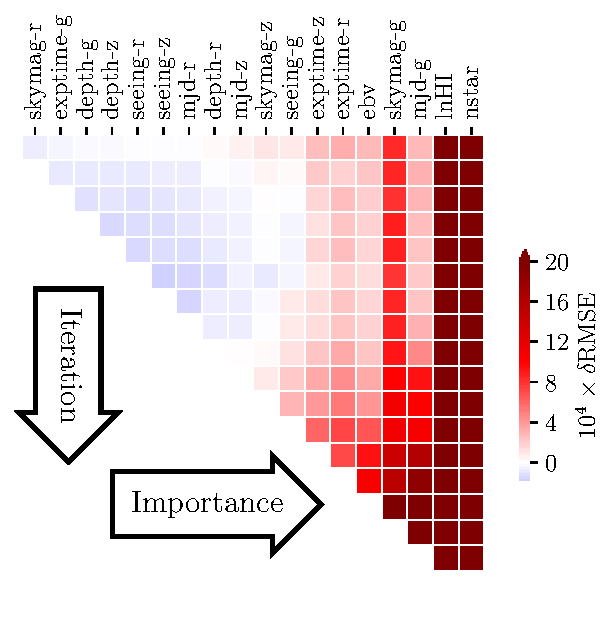
\includegraphics[width=0.4\textwidth]{dr7ablation.pdf}
    \caption{Feature importance based on backward feature elimination for the first partition, as an example. This process iteratively removes the feature whose removal produces the largest decrease in the validation RMSE (i.e., the greatest improvement in fitting) until no decrease is observed. After the first iteration of removal (the top row), the removal of $skymag-r$ decreased the validation RMSE the most and therefore $skymag-r$ is removed. In the second iteration (the second row), removing $exptime-g$ decreased the validation RMSE the most and therefore it is removed. However, in the ninth iteration, the removal of $mjd-z$ did not decrease the validation RMSE and therefore the feature selection stops here, passing the rightmost ten features to the neural network regression. As a result of the process, the importance increases from left to right, and the rightmost ten maps in the figure ($ebv$, $nstar$, $logHI$, $seeing-g$, $skymag-g$, $skymag-z$, $exptime-r$, $exptime-z$, $mjd-g$, $mjd-z$) are the ones that worsen the validation RMSE when being removed from the input layer.}
    \label{fig:dr7ablation}
\end{figure}

\begin{figure}
    \centering
    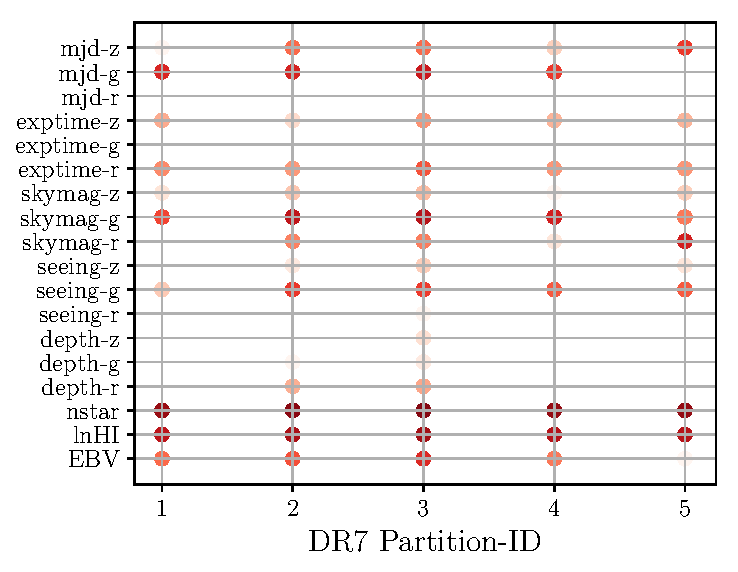
\includegraphics[width=0.45\textwidth]{hyper-params_data.pdf}
    \caption{Important imaging maps identified by the backward feature elimination (\textit{feature selection}) procedure for the five partitions used for the DR7 dataset. A darker color of a point within each partition represents a more important attribute identified by the feature selection procedure. Note that $nstar$ is identified as the most important attribute in all partitions, i.e., across the footprint.}
    \label{fig:dr7ablation2}
\end{figure}
 

\subsubsection{Hyper-parameter tuning, training, and testing}

We train the hyper-parameters for each partition separately. At each training epoch and for each choice of hyper-parameters, we apply the trained network on the validation fold. We adjust the hyper-parameters accordingly such that the validation MSE is minimized. Our neural network has the following five hyper-parameters: number of hidden layers; number of training epochs $N_{{\rm epoch}}$; L2 regularization scale $\lambda$; batch size $N_{{\rm batch}}$; Adam's learning rate. We tune one hyper-parameter at a time. To find the optimal learning rate, we monitor the behavior of the cost function during training. We observe that a learning rate of 0.001 leads to a smoothly decreasing cost function vs. training epochs. We train the network for up to $N_{\rm epoch} = 500$ epochs although we implement the early stopping technique with the inertia (or patience) of 10 and the tolerance of 1.e-4: this means the training will be stopped if none of the last 10 epochs achieved a smaller relative error reduction with respect to the minimum validation error, within the tolerance. For the number of hidden layers, we try the following architectures, in which the total number of hidden neurons is fixed at 40 (i.e. roughly twice the number of the features) except for the linear model:\\~\\
%
%
$[0]$  : no hidden layers \\
$[40]$ : one hidden layer of 40 neurons \\
$[20, 20]$ : two hidden layers of 20 neurons on each \\
$[20, 10, 10]$ : three hidden layers of 20, 10 and 10 neurons \\
$[10, 10, 10, 10]$ : four hidden layers of 10 neurons\\~\\
After finding the best number of layers, we proceed to tune $\lambda$ by trying  powers of 10, e.g., 0.001, 0.01, ..., 1, ..., 1000. Finally, we adjust $N_{\rm batch}$ by trying powers of 2, e.g., 128, 256, ... , 4096. The optimal set of the hyper-parameters for each partition is summarized in Tab. \ref{tab:hparams}.\\

\begin{table}
	\centering
	\caption{The best hyper-parameters for each partition.}
	\label{tab:hparams}
	\begin{tabular}{lccr} % four columns, alignment for each
	    \hline
		\hline
		Partition/Hyper-parameter & number of layers & $\lambda$ & $N_{\rm batch}$ \\
		\hline
		1 & [20, 20] & 0.001 & 4096\\
		2 & [20, 10, 10] & 0.001 & 512\\
		3 & [20, 10, 10] & 0.001 & 1024 \\
		4 & [20, 10, 10] & 0.001 & 512 \\
		5 &  [20, 10, 10] & 0.001 & 2048\\
		\hline
		\hline
	\end{tabular}
\end{table}

Once the optimal set of hyper-parameters is identified, the network is trained with these hyper-parameters for 10 independent runs, each one with a different initialization of the weights and biases, and then applied on the test set. We compute the median of the predicted test label from the 10 runs, and aggregate the results over the 5 different partitions to construct the map of the predicted label ($\hat{\mathcal{F}}$) for the entire footprint. For our default method, the backward feature elimination is conducted for each partition and reduces the number of input features before the hyper-parameter training step, as illustrated in Fig.~\ref{fig:splitapp}.  This process is performed for each partition separately, each partition using a different fold as the test set, until the entire footprint is covered through the 5 test folds. The flow of the feature selection, hyper-parameter tuning, and testing is summarized in Fig. \ref{fig:splitapp}.\\

\begin{figure*}
         \centering
         \includegraphics[ width=0.95\textwidth]{split.pdf}
         \caption{A flow-chart of the backward feature elimination and hyper-parameter tuning for each partition. This entire process is performed five times for each of the five partitions/permutations such that the entire footprint is covered by aggregating different testing folds. }
         \label{fig:splitapp}
\end{figure*}

% multivariate
\subsection{Mitigation with Multivariate Linear Functions}
We use linear and quadratic polynomial functions to model the normalized galaxy density dependence on the imaging attributes (Eq.~\ref{eq:tfs}), as the benchmark approaches to be compared with the neural network. Unlike the proposed neural network method, no regularization or dimensionality reduction is performed, and all data are used to train the parameters of the regression models. Despite a lack of any deliberate machinery against over-fitting, we note that over-fitting is less likely to be an issue for this method since the size of the data is much greater than the number of the fitting parameters. Nevertheless, we tried splitting the sample into 60\% of the training data to derive the best fit linear coefficients and 20\% of the test set (i.e., the same training and test sample size to have a fair comparison with the neural network) to apply the derived coefficients and permuted five times until the test set covers the entire footprint. We find that such split does not change the results of the linear regression. On the other hand, the limited flexibility of its parameterized form could be a weakness of this method and we believe it is responsible for the differences that the neural network method makes in the comparison that we show in Section \ref{sec:mitigateDR7}.\\

The contamination model from Eqs.~\ref{eq:nnbar} and ~\ref{eq:tfs} can be estimated via a multivariate linear function in terms of the standardized imaging attributes (\textbf{s}) as,

\begin{equation}\label{eq:multvar}
\hat{\mathcal{F}}(\textbf{s}|b_{0},\alpha) = b_{0} + \sum_{m=1}^{M}\sum_{k=1}^{18} \alpha_{mk} (\frac{s_{k}-\overline{s_{k}}}{\sigma_{k}})^{m} ,
\end{equation}
where $M$ is the maximum power law index equal to 1 and 2 for the linear and quadratic polynomial model, respectively; the constants $\overline{s_{k}}$ and $\sigma_{k}$ are respectively the mean and standard deviation of the k'th imaging quantity, $s_{k}$ (see Tab. \ref{tab:meanstats}). The parameters $b_{0}$ and $\alpha_{mk}$ are the intercept and the corresponding coefficients\sout{s} for each term, respectively, which are tuned by minimizing the weighted sum of the squared errors. The output of the regression is applied as the selection mask on the observed galaxy density to eliminate the systematic effects (see Eq., \ref{eq:wsys}).\\

\subsection{Angular Clustering Statistics}\label{subsec:ang_clustering}
\subsubsection{One point statistics}
In the absence of the systematic effects, the galaxy density field should be independent from the imaging attributes and will only depend on the cosmological fluctuations. When averaged over many spatial positions, the cosmological fluctuations will be averaged out and therefore the average density should be equal to the mean density once the survey footprint is accounted for. A deviation from the mean density as a function of the imaging attributes therefore is indicative of the average dependence of the observed galaxy density on the corresponding imaging attributes. To assess the level of the contamination in the data, we compute the histogram of the spatially averaged galaxy density vs the imaging attributes. For each of the system attribute, $s_k$, we prepare 20 bins. For each bin of $s_{k}$, we have:

\begin{equation}\label{eq:nnbar_stat}
    \frac{\overline{n}(s_{k})}{\overline{n}_{tot}} \equiv \frac{1}{\hat{\overline{n}}}~ \frac{\displaystyle\sum_{s_{k}\leq s_{k,i}<s_{k}+\Delta s_{k}} n^{o}_{i}}{\displaystyle\sum_{s_{k}\leq s_{k,i}<s_{k}+\Delta s_{k}} f_{\rm pix, i}},
\end{equation}
where the indices $i$ and $k$ respectively represent the pixel index, and the systematic index; $\Delta s_{k}$ is the bin width arranged for different $s_k$ bins such that each bin contains almost the same amount of effective area, in an attempt to suppress fluctuations in $\overline{n}(s_{k})/\overline{n}_{tot}$ due to small number statistics. We estimate the error bars using the Jackknife resampling of 20 non-contiguous subsamples of pixels within each imaging attribute bin ~\citep[see e.g.][]{ross2011ameliorating}:


\begin{equation}\label{eq:error_jack}
    \sigma^{2}_{{\rm Jack}}(s_{k}) = \frac{19}{20}\sum_{j=1}^{20} \left[    \frac{\overline{n}(s_{k})}{\overline{n}_{tot}} -     \frac{\overline{n}_{j}(s_{k})}{\overline{n}_{tot}}\right]^{2}  ,
\end{equation}
 where $\overline{n}_{j}(s_{k})/\overline{n}_{tot}$ is computed over the entire sample when the $j$'th Jackknife region is excluded.
As a result of the adjusted $\Delta s_{k}$, the level of $\sigma^{2}_{{\rm Jack}}(s_k)$ is almost the same for all $s_k$. Under a successful mitigation of the systematic effects, one expects that the corrected density field is independent of the imaging attributes, i.e., $\overline{n}(s_{k})/\overline{n}_{tot}$ being consistent with unity.


\subsubsection{Two-point clustering statistics}
The two-point clustering statistic measures the spatial correlation of the galaxy density, and has been the main statistic for extracting the cosmological information from galaxy surveys. We use the angular auto and cross two-point clustering statistics of the galaxy density field as well as of the imaging attributes to estimate the impact of the potential systematics on the cosmological clustering signal and to examine the effectiveness of the mitigation techniques tested in this paper. For pixel $i$, we calculate the galaxy overdensity $\delta_{i}$ using Eq.~\ref{eq:overden} and the fluctuation of a given imaging attribute $\delta^{s}_{i}$ as
\begin{align}\label{eq:delta}
    \hat{\delta}^{s}_{i} &= \frac{s_{i}}{\hat{\overline{s}}} - 1 ,
\end{align}
where $\hat{\overline{s}}$ is the mean of each imaging attribute weighted with $f_{{\rm pix},i}$,
\begin{align}\label{eq:deltasysbar}
\hat{\overline{s}} = \frac{\sum_i f_{{\rm pix},i} s_i}{\sum_i f_{{\rm pix},i}}
\end{align}
following \citet{ross2011ameliorating}.\\

By definition, Eqs.~\ref{eq:nbar} and \ref{eq:delta} ensure that the following integral of the observed quantity over the entire footprint vanishes:
\begin{align}\label{eq:ic}
    \sum_{i} \hat{\delta}_{i}~f_{{\rm pix},i} = 0,
\end{align}
for both the galaxy as well as imaging attribute fluctuations. We utilize both the angular correlation function and angular power spectrum to extract the cosmological information from the galaxy density field.


\begin{itemize}
    \item Angular Correlation Function: we employ the healpix-based estimator to compute the angular correlation function which, for a separation angle $\theta$, is defined as \citep[see e.g.][]{scranton2002analysis,ross2011ameliorating}
    \begin{align}
        \omega^{p,q} (\theta) = \frac{\displaystyle\sum_{ij} \hat{\delta}^{p}_{i} \hat{\delta}^{q}_{j} \Theta_{ij}(\theta) f_{\rm pix, i}f_{\rm pix, j}}{\displaystyle\sum_{ij} \Theta_{ij}(\theta) f_{\rm pix, i}f_{\rm pix, j}},\label{eq:ancor}
    \end{align}
    where $p=q$ gives an auto correlation function estimator, $p\neq q$ gives a cross correlation function estimator, and $\Theta_{ij}$ is one when two pixels $i$ and $j$ are separated from each other within $\theta$ and $\theta+\Delta\theta$, or zero otherwise. Note that our estimator weighs each pixel overdensity with $f_{{\rm pix}, i}$ since the pixels with a greater complete area coverage should have a higher signal to noise. Such weight is straightforwardly corrected by the denominator in Eq.~\ref{eq:ancor} unlike its conjugate estimator (i.e., the power spectrum). Since our overdensity map resolution is limited by the pixel size, we set the $\Delta\theta$ to be the resolution of a pixel ($\sim$ 0.23 deg). We use the Jackknife resampling technique with 20 equal-area contiguous regions, as shown in Fig. \ref{fig:jackknifes}, to estimate the error-bars on $\omega (\theta)$ (see Eq. \ref{eq:error_jack}). \\
    \begin{figure}
        \centering
        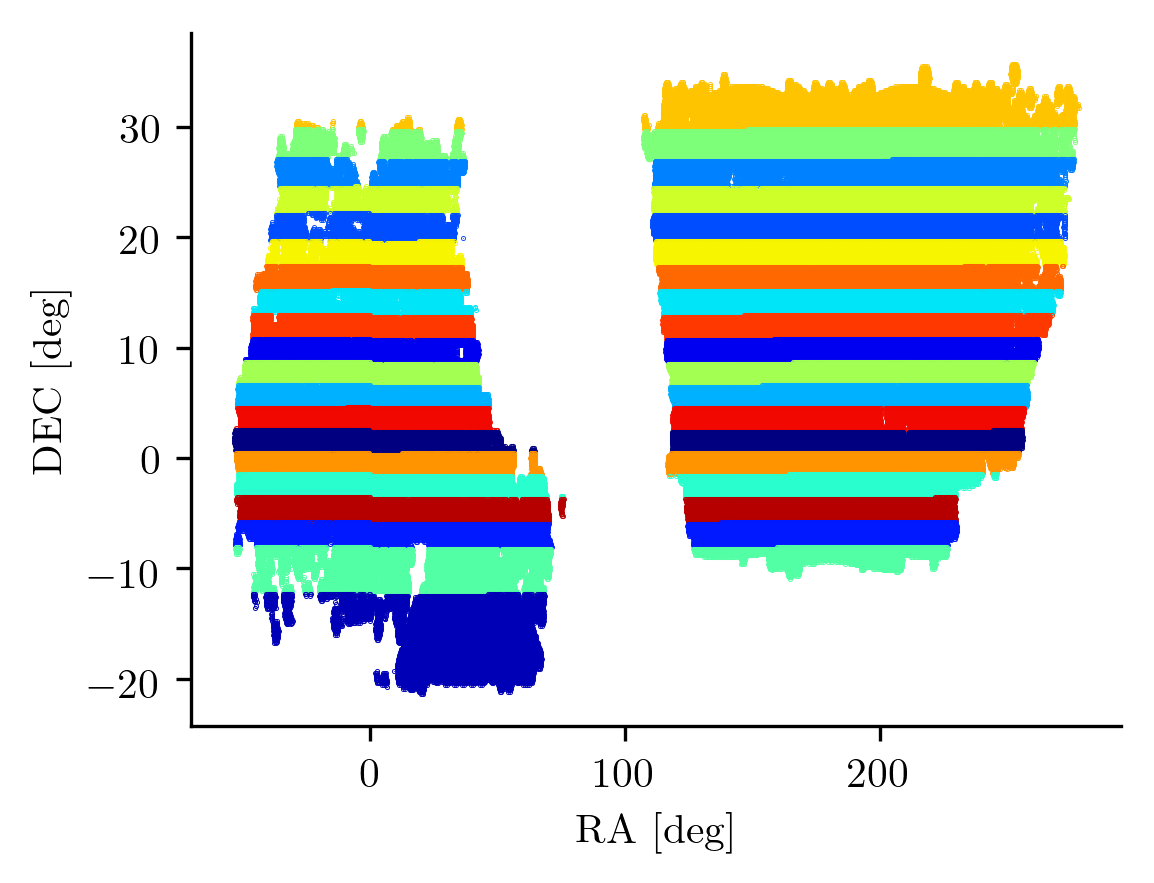
\includegraphics[width=0.4\textwidth]{jackknifes.png}
        \caption{Twenty equal-area contiguous regions used to estimate the Jackknife errorbars for the 2D clustering statistics.}
        \label{fig:jackknifes}
    \end{figure}


    \item Angular Power Spectrum : one can conveniently expand a coordinate on the surface of a sphere in terms of spherical harmonics or, if azimuthally symmetric, Legendre polynomials. We define the following estimator for expanding the galaxy overdensity:
    \begin{equation}
        \hat{\delta}_{i} = \sum_{\ell=0}^{\ell_{{\rm max}}}\sum_{m=-\ell}^{\ell} a_{\ell m} Y_{\ell m}(\theta_{i}, \phi_{i}),
    \end{equation}
    where $\theta, \phi$ represent the polar and azimuthal angular coordinates of pixel \textit{i}, respectively. The cutoff at $\ell=\ell_{{\rm max}}$ assumes that the signal power is not significant for modes $\ell>\ell_{{\rm max}}$. We define the following spherical harmonic (SH) transform estimator of overdensity ($\hat{\delta}$) over the total number of non-empty pixels $N_{{\rm pix}}$:
   
    \begin{equation}
        \hat{a}_{\ell m} = \frac{4\pi}{N_{{\rm pix}}} \sum_{i=1}^{N_{{\rm pix}}}  \hat{\delta}_{i}~f_{\rm pix, i}~ Y^{*}_{\ell m}(\theta_{i}, \phi_{i}),
    \end{equation}
    where $^{*}$ represents the complex conjugate, and we again down-weight the overdensity in pixel \textit{i} by the completeness ($f_{\rm pix, i}$). Due to the survey window function implicit in the sum over the non-empty pixels and explicit in $f_{\rm pix, i}$, our estimator would not return unbiased estimates of the SH coefficients, unless the window function effect is corrected for, and also the expected orthogonalities between different SH modes would not hold. Nevertheless, we define the angular power spectrum estimator as the average of the magnitude of SH coefficients over $m$:
    \begin{equation}
        \hat{C}^{p,q}_{\ell} = \frac{1}{2\ell +1} \sum_{m=-\ell}^{\ell} \hat{a}^{p}_{\ell m} \hat{a}^{q*}_{\ell m},
    \end{equation}
    where $p=q$ gives an auto power spectrum, $p\neq q$ gives a cross power spectrum between the galaxy density and the imaging attributes. In order to compute the angular power spectrum, $C_{\ell}$, we make use of the ANAFAST function from HEALPIX \citep{gorski2005healpix} with the third order iteration of the quadrature to increase the accuracy\footnote{We refer the reader to \url{https://healpix.sourceforge.io/pdf/subroutines.pdf}, page 104.}. 
    Unlike in the angular correlation function, we do not attempt to correct for the survey window function/survey mask effect in the angular power spectrum both for the DR7 data and the mocks. Instead, for the mock test, we use the angular power spectrum without the contamination model, i,e, the `Null' case, as our baseline to compare with different mitigation methods.\\ 
    
    For both the mock and real datasets, we also utilize the cross power spectra between the galaxy density and various imaging maps to evaluate the performance of the  mitigation. In order to estimate the significance of the contamination in $\hat{C}^{g,g}_{\ell}$ (or $\omega^{g,g} (\theta)$) before and after mitigation, we calculate $[\hat{C}^{g,s_k}_{\ell}]^2/\hat{C}^{s_k,s_k}_{\ell}$ (or $[\omega^{g,s_k}(\theta)]^2/\omega^{s_k,s_k}(\theta)$) as a proxy.~\footnote{These quantities would be the true level of contamination to $\hat{C}^{g,g}$ if the contamination model is linear and systematics are independent from one another~\citep{ashley2012MNRAS,2012ApJ...761...14H}.}
\end{itemize}

\def\ihMpc{h^{-1}{\rm Mpc}}
\def\trihMpc{h^{3}{\rm Mpc}^{-3}}
\subsection{Survey Mocks}\label{subsec:surveymocks}
Imaging systematics tend to affect the clustering signal mainly on large scales \citep{myers2007clustering, huterer2013calibration} and the distribution of galaxies on large scales at moderately low redshift can be well-approximated by a log-normal distribution~\citep{1991MNRAS.248....1C}. We therefore believe that log-normal mocks would be sufficient for the purpose of validating our systematic mitigation techniques. We use the \textit{Nbodykit} package \citep{hand2017nbodykit} to generate one hundred log-normal cubic mocks with the box-side length of $5274 \ihMpc$ and $1024^3$ mesh cells, with the input power spectrum matched to the linear power spectrum  at $z=0.85$ based on the \textit{Planck 2015} cosmology~\citep{ade2016planck} (i.e., flat $\Lambda$CDM with $\Omega_m=0.3089 \pm 0.0062$, $H_{0}=67.74 \pm 0.46$, $\sigma_8 = 0.8159 \pm 0.0086$), with the galaxy bias of 1.5 and the volume density of $1.947\mathrm{e}{-4}\trihMpc$ \citep[see e.g.][]{Raichoor2017MNRAS.471.3955R}. Then, we use the \textit{make\_survey} package \citep{white2013mock} to sub-sample the mock galaxies based on the NGC eBOSS ELG redshift distribution in \citet{Raichoor2017MNRAS.471.3955R} with the redshift cut of  0.55 < z < 1.5 and to transform the cubic mocks into survey-like mocks. We do not include redshift-space distortions (RSD) in the mocks as we believe that the systematics mitigation efficiency does not depend on  the presence of RSD.\\

The survey mocks are then projected onto the two-dimensional sky using HEALPIX and overlaid on the NGC footprint of the DECaLS DR7 dataset to be assigned with the DR7 imaging attributes. Fig. \ref{fig:mock_on_dr} illustrates the resulting projection of a simulated survey mock and the DECaLS DR7 data. Note that the mock footprint (89672 pixels) is smaller than the DECaLS DR7 data (187257 pixels) almost by a factor of 2. We only use the pixels of the mock that have the DR7 imaging attributes available. The holes (e.g., RA and DEC around 200 and 5 deg) are the pixels that do not have the imaging attributes from the real data. In order to account for the mock survey footprint, we distribute 2500 random points per deg$^{2}$ within the mock footprint and derive the completeness map for the mocks.


\begin{figure}
    \centering
    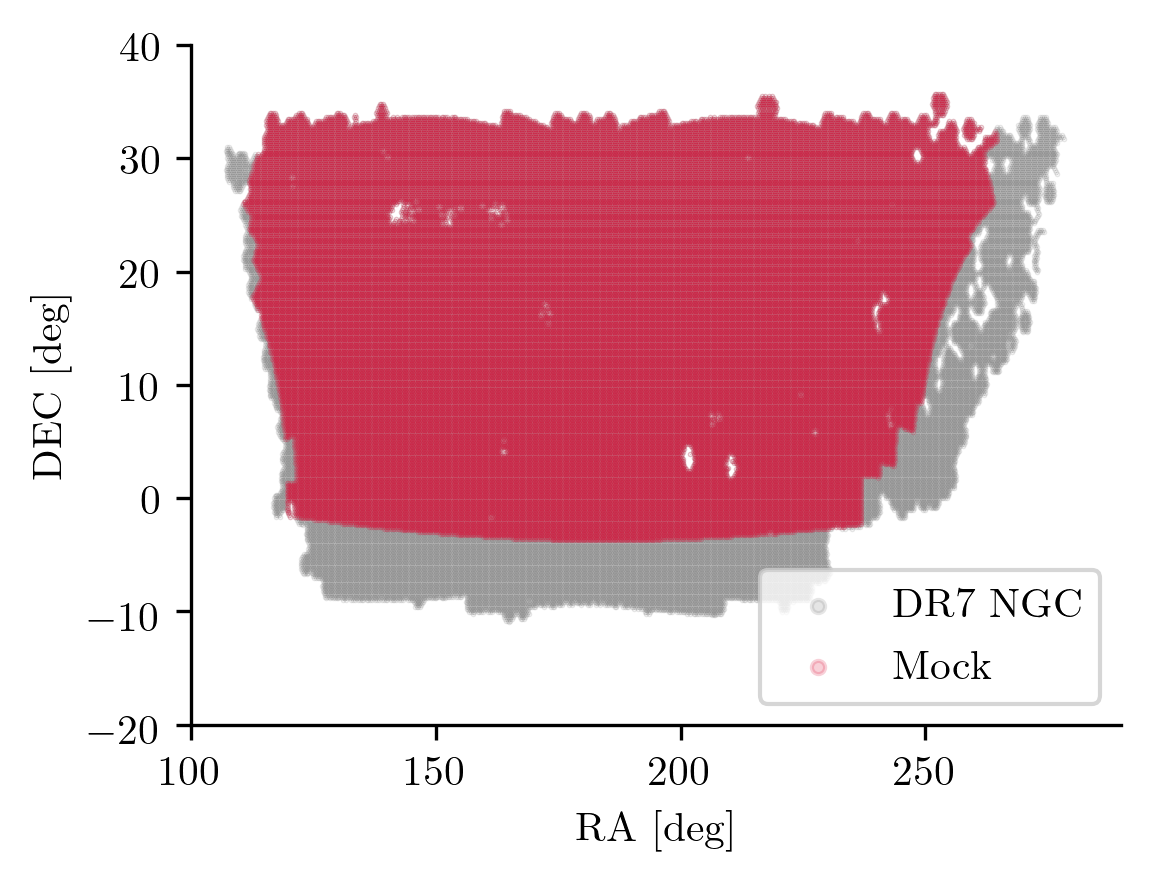
\includegraphics[width=0.45\textwidth]{mockondr.png}
    \caption{The projection of the mock footprint (blue) onto the North Galactic Cap of the DECaLS DR7 footprint (gray). With this projection, the imaging attributes from the real data are assigned to the mocks.}
    \label{fig:mock_on_dr}
\end{figure}


\subsubsection{Null Mocks}
A good mitigation technique should minimally remove the true cosmological signal. One way of ensuring this is to check if the mitigation method returns the true clustering in the presence of contaminations, which will be tested using the contaminated mocks. Another way is to check if the mitigation method correctly makes a null operation on the clustering in the absence of contaminations, returning $\hat{\mathcal{F}}\simeq 1$. To this end, we utilize the 2D projected mocks without introducing any modulation due to imaging attributes in the galaxy density fields. Henceforth, we call this set of simulations, \textit{null} mocks.\\

Fig.~\ref{fig:ngal_hist} shows the pixel distribution histograms of the number of galaxies per pixel of the mocks in comparison to that of the DECaLS DR7 data on the common footprint. The average $ngal=7.0/{\rm pixel}$ of the null mocks is smaller than $ngal=13.3/{\rm pixel}$ of the DECaLS DR7 data (even after accounting for the 5\% loss due to tiling completeness and 27\% loss due to the redshift range, as stated in \citet{Raichoor2017MNRAS.471.3955R}). We believe that the difference in $ngal$ is due to the different \textit{clean photometry} criteria applied to the ELG selection in \citet{Raichoor2017MNRAS.471.3955R} and to the targets in this paper. The standard deviation of $ngal$ of the null mocks is 3.0, which is smaller than 4.6 of the DECaLS DR7 ELGs.

\subsubsection{Contaminated Mocks}
We modulate the mock galaxy density fields using imaging attributes of the DECaLS DR7 data and generate the contaminated mocks with additional random noise. The modulation is done based on the best fit coefficients of the imaging attributes and their covariances for $\mathcal{F}$ (Eq.~\ref{eq:nnbar}) that we derived from the DECaLS DR7 data using our fiducial linear regression model.\\

In detail, we pick the 10 imaging attributes, i.e., $EBV$, $nstar$, $lnHI$, $seeing-g$, $skymag-g$, $skymag-z$, $exptime-r$, $exptime-z$, $mjd-g$, $mjd-z$ of the DECaL DR7 data, which were selected from the feature selection procedure on one of the partitions, and modulate the mock density field $n$ with $\mathcal{F}$ that is derived from random deviates of the imaging attribute coefficients while accounting for their covariances. Since the measured covariance of such quantities includes both the cosmological fluctuation and the fluctuations due to the imaging attributes, we rescale the measured covariance matrix of the systematics such that the random fluctuation in $ngal$ per pixel due to contamination is at a similar level to the cosmological fluctuation from the null mocks. As a result of the random fluctuation in the contamination model we introduced, some of the pixels will be assigned negative galaxy number. We drop these pixels from our sample. This removes 3.1\% of the mock footprint, reducing our mock footprint size from 89672 to 86875 pixels. We then introduce Poisson process, i.e., another random variation step, to ensure the modulated galaxy number per pixel is an integer. These two random variation processes increase the noise in the mock datasets such that the standard deviation of $ngal$ of the contaminated mocks ($=4.4$) is almost the same as that of the DR7, despite the different average $ngal$ (Fig.~\ref{fig:ngal_hist}).\\


Therefore our mock contamination is simpler than the DECaLS DR7 data in that we adopted a linear model, which is chosen purposely since we do not want to give a priori advantage to our neural network method and also since all methods are capable of reproducing the linear model. Meanwhile, this setup is more challenging than the DECaLS DR7 data since the mitigation is conducted in the presence of a greater level of noise. Note that, while we included only 10 dominant imaging attributes in the contamination, the remaining attributes in the DECaLS data are correlated with these 10 and therefore with the modulated galaxy density. The mitigation in the following mock test will be challenged to deal with such indirect correlations among the 18 attributes. 


\begin{figure}
    \centering
    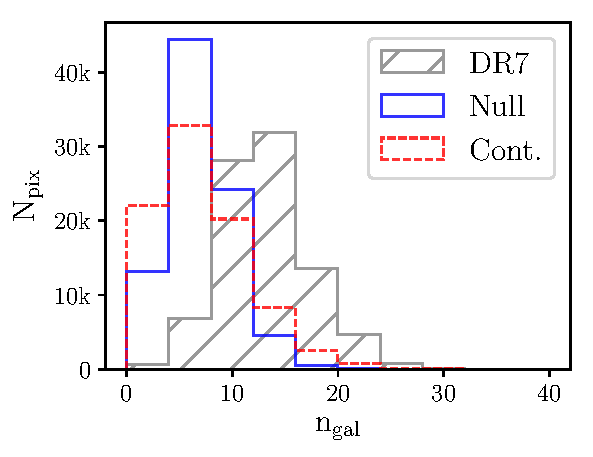
\includegraphics[width=0.4\textwidth]{ngal_hist.pdf}
    \caption{Histogram of the number of galaxies per pixel for DR7 (hatched grey), null (solid blue), and contaminated (dashed red) mocks. All distributions are corrected for the pixel completeness $f_{\rm pix}$. The DR7 distribution is scaled down to account for 5\% tiling completeness, and 27\% to 0.55 < reliable redshift <1.5. The residual difference between the mocks and the DR7 shown here might be due to differences between the \textit{clean photometry} criteria applied to eBOSS target selection and those we apply to DR7.}
    \label{fig:ngal_hist}
\end{figure}{}
\section{Results}\label{sec:results}
In this section, we present the measurements of the clustering statistics before and after correcting for the systematic effects for the real dataset as well as the simulated ones. We demonstrate that the neural network is capable of learning more structure in the observed galaxy density field due to its greater flexibility beyond a fixed functional form, and therefore it can eliminate more excess clustering which is believed to be due to the imaging systematics. We then show the performance of the neural network and multivariate linear models when applied on the mock datasets.

\subsection{Mitigating systematics from the DECaLS DR7 Data}
\label{sec:mitigateDR7}
In the left panel of Fig. \ref{fig:weights}, we show the pixel distribution histograms of the selection mask from the three different regression models we consider in this paper. While all three models show fairly consistent selection masks for most of the pixels (note the logarithmic scaling of $Npix$), the neural network method returns extended tails due to a higher representation flexibility associated with its nonlinear nature.  We remove pixels with $\hat{\mathcal{F}} < 0.5$ or $> 2.0$ from our data to avoid too aggressive selection correction since we believe none of these methods can be accurate enough for such long baseline extrapolation. These pixels account for 1.0\% of the original data (from 187257 to 185781 pixels). In the right panel, we show the spatial distribution of the removed pixels in the case of the neural network selection mask. \\

\begin{figure*}
    \centering
    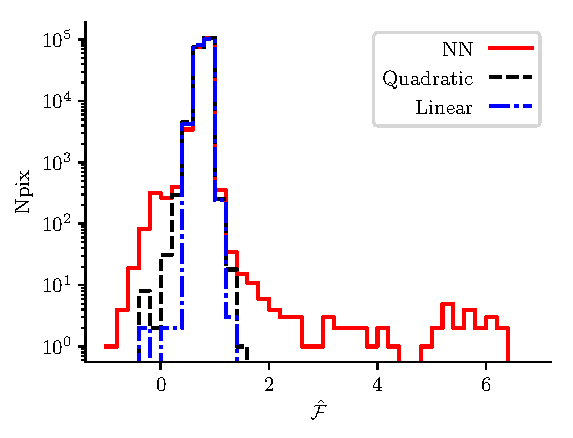
\includegraphics[width=0.4\textwidth]{w_dr7.pdf}
    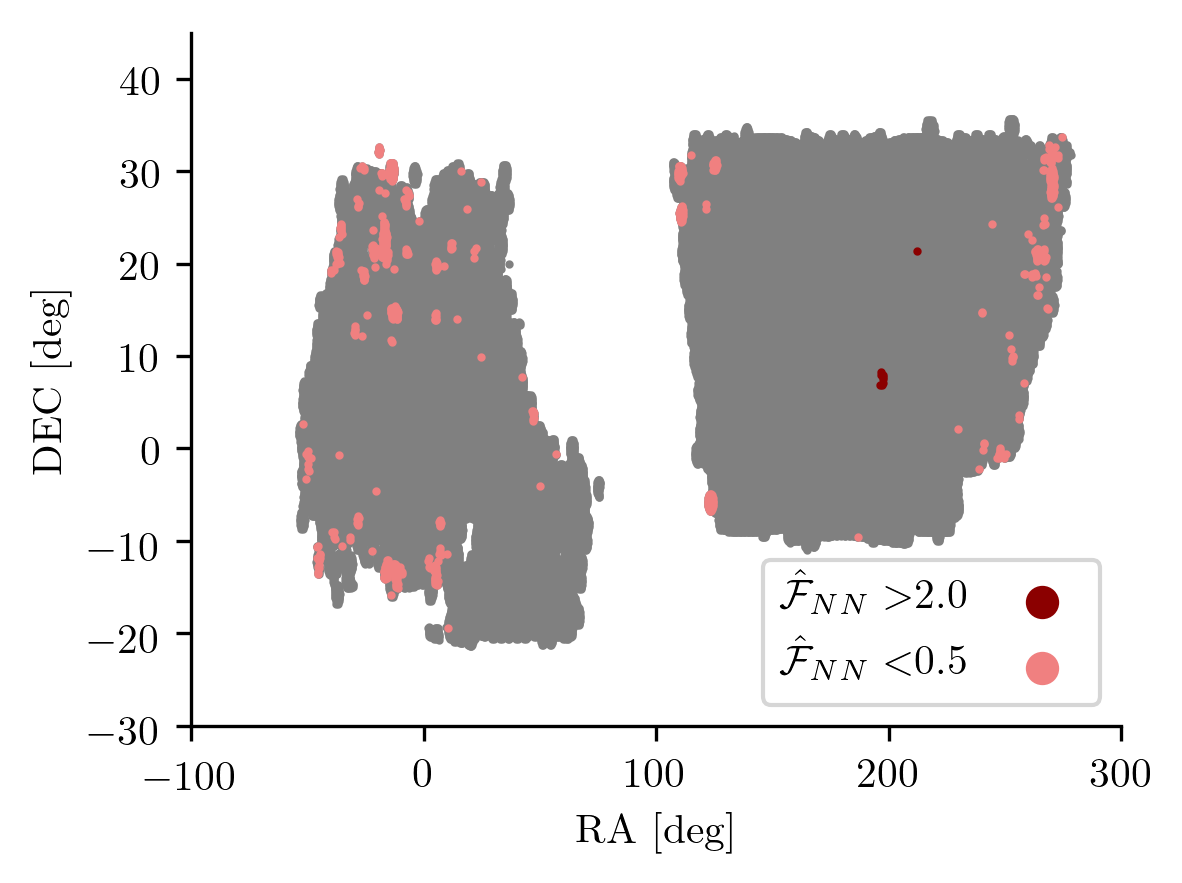
\includegraphics[width=0.4\textwidth]{w_dr7_extremes.png}
    \caption{\textit{Left}: Distribution of the selection masks (i.e., estimates of the contamination model) derived from different regression models. \textit{Right}: Spatial scatter of the pixels we remove from our data due to the extreme values of the neural network selection mask.}
    \label{fig:weights}
\end{figure*}


Fig. \ref{fig:density_selection} illustrates the spatial distribution of the observed galaxy density before (top left) and after correction (top right) using the neural network selection mask. The bottom panels show the neural network selection mask used for the correction (left) in comparison to the masks derived from the linear (middle) and the quadratic polynomial (right) models. All three masks capture a very similar large scale pattern such as the decrease in the galaxy density close to the Galactic midplane, which is consistent with the negative correlation coefficients between the galaxy density and the Galactic extinction, hydrogen column density, or stellar density. On smaller angular scales, the three selection masks show different fluctuation details. In the following analyses, we examine which method returns the least contaminated galaxy density distribution. \\

\begin{figure*}
    \centering
    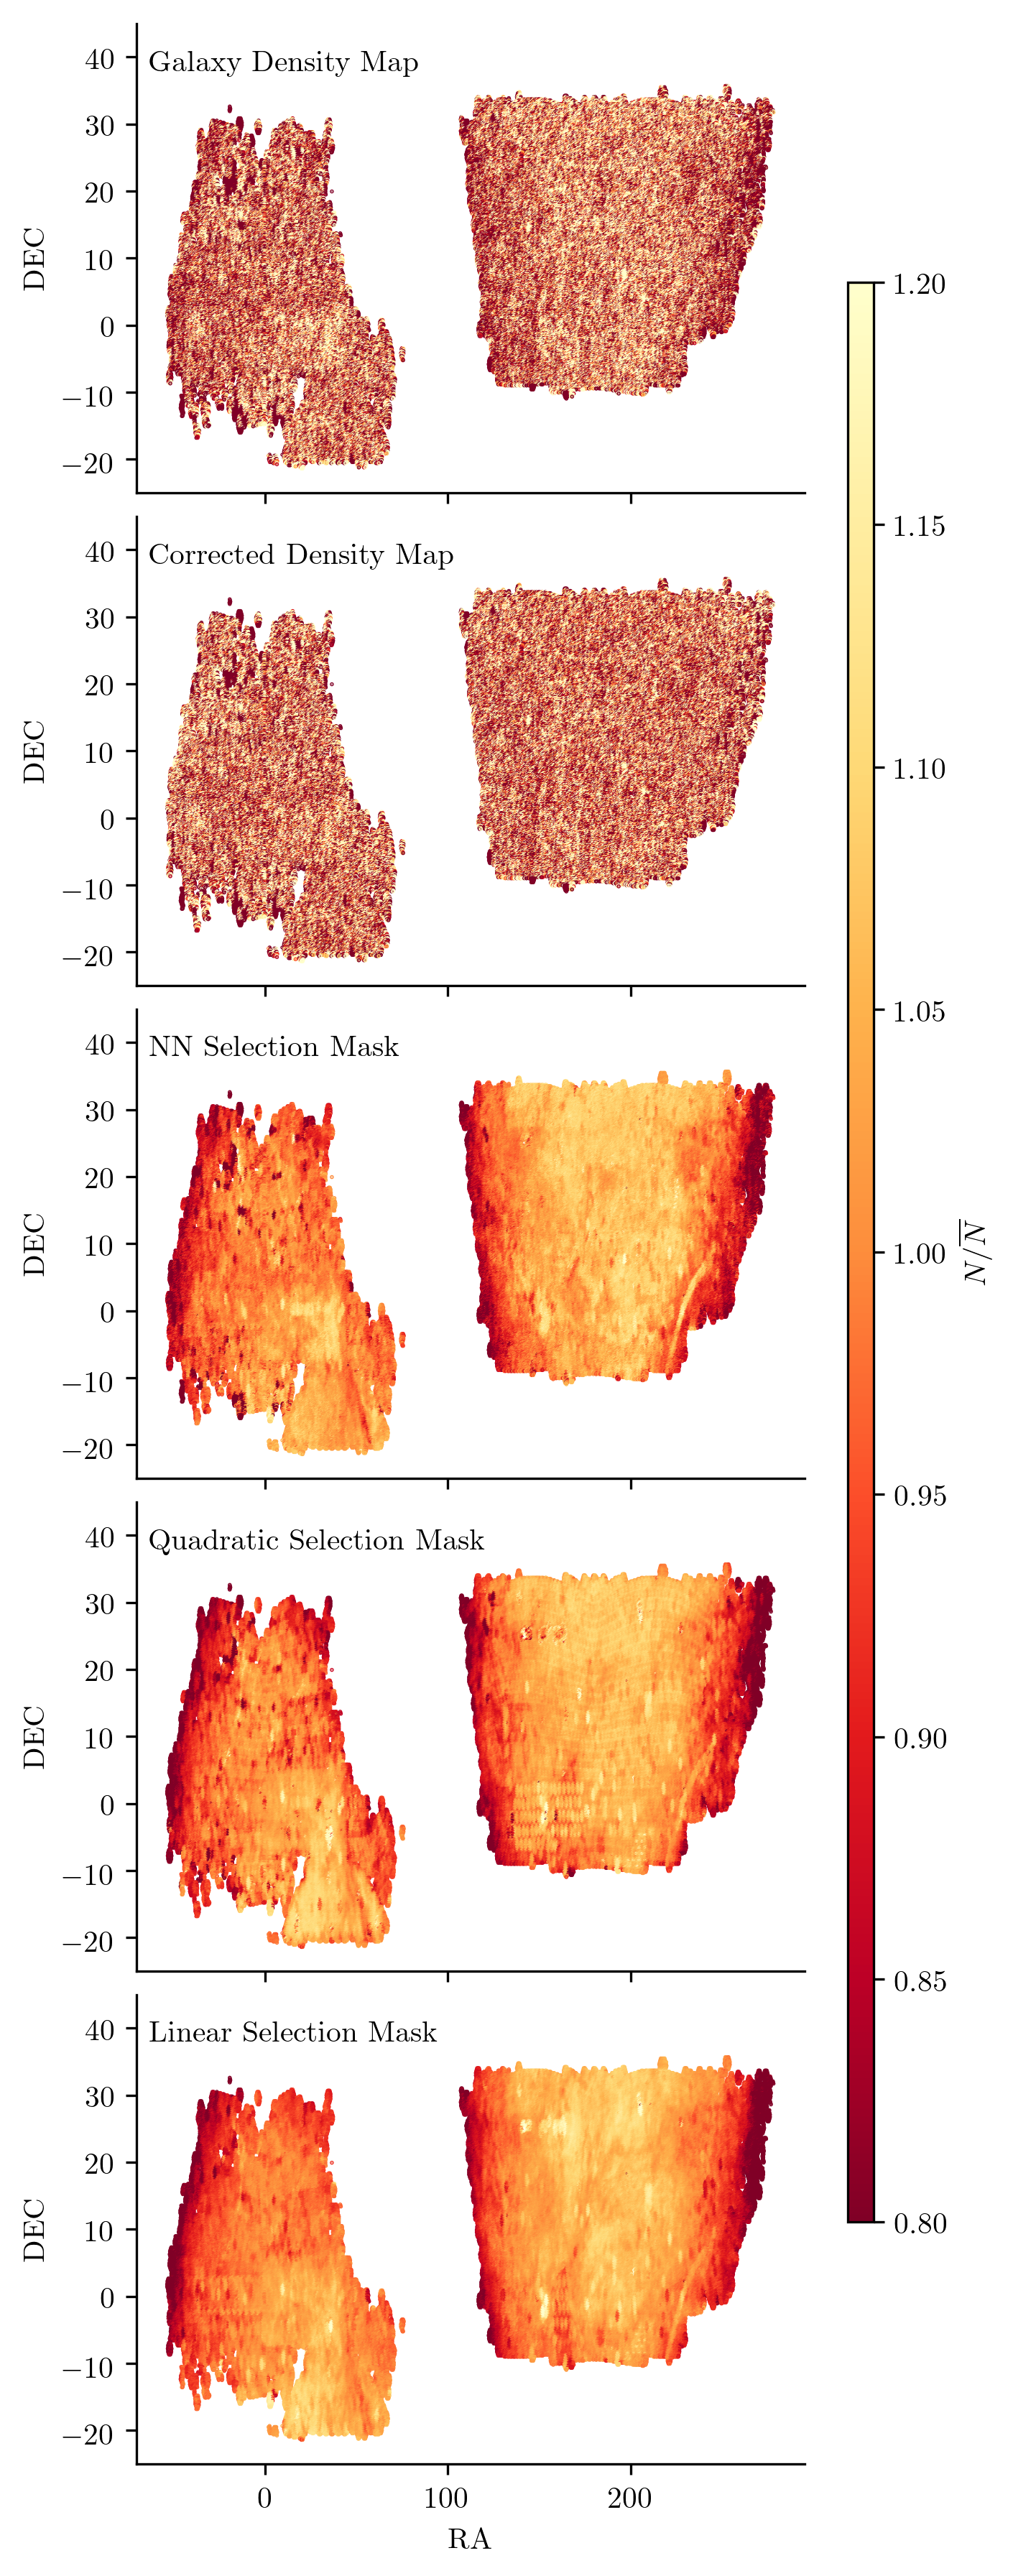
\includegraphics[width=0.98\textwidth]{deltas.png}
    \caption{\textit{Top}: the normalized observed galaxy density and corrected density map using the neural network selection mask from left to right, respectively. \textit{Bottom}: the selection masks from the Neural Network, quadratic, and linear polynomial models, respectively from left to right. All three selection masks are able to capture the behavior that the galaxy density systematically drops at the footprint boundaries i.e., high extinction regions.}
    \label{fig:density_selection}
\end{figure*}

First, once the systematic effects are corrected for, the mean galaxy density should be independent of the imaging attributes. In Fig. \ref{fig:nnbar} we show the number density of galaxies as a function of the imaging attributes. Again, different bins are set to include the same effective pixel area and therefore have the same sampling error. The solid black curve shows the galaxy mean density before correction and the solid red shows the result after correction with the selection mask of the neural network model. The dot-dashed curve represents the correction using the linear polynomial model and the dashed curve is for the the quadratic polynomial model. The errorbars are computed using 20 Jackknife sub-samples, and shown on only one case for clarity. Similar to what we found from the feature selection procedure, the stellar density, Galactic extinction, and HI density exhibit the strongest dependence before correction. After correction, all three methods return the fractional galaxy density close to unity. To quantify the deviation from unity, we report the $\chi^{2}$ statistics while ignoring the covariance between different bins and different imaging attributes in Tab.~\ref{tab:chi2}. Overall, the neural network achieves the smallest deviation from unity which indicates its highest efficiency in reducing the systematic effects.\\

\begin{table}
	\centering
	\caption{We use the $\chi^{2}$ statistic to quantify the performance of each mitigation method based on $\overline{n}/\overline{n}_{tot}$ vs. systematics (see. Fig. \ref{fig:nnbar}). In this table we show the cumulative value over all bins and all imaging attributes (i.e., $N_{\rm bins}=$20 bins $\times$ 18 attributes) without accounting for the covariance both between the imaging maps and between different bins. Note that the best fit neural network model was applied to the unseen data (i.e., the test set) unlike in the linear and quadratic polynomial models. Nevertheless the neural network method returns the smallest $\chi^{2}$, i.e., the highest efficiency.}
	\label{tab:chi2}
	\begin{tabular}{lccr} % four columns, alignment for each
	    \hline
		\hline
		Correction scheme & $\chi^{2}$ & $N_{\rm bins}$ & $\chi^{2}/N_{\rm bins}$ \\
		\hline
		None & 20921.633 & 360 & 58.116\\
		Linear & 2588.349 & 360 & 7.190\\
		Quadratic & 2623.006 & 360 & 7.286 \\
		Neural Network & 966.601 & 360 & 2.685\\
		\hline
		\hline
	\end{tabular}
\end{table}


\begin{figure*}
\centering
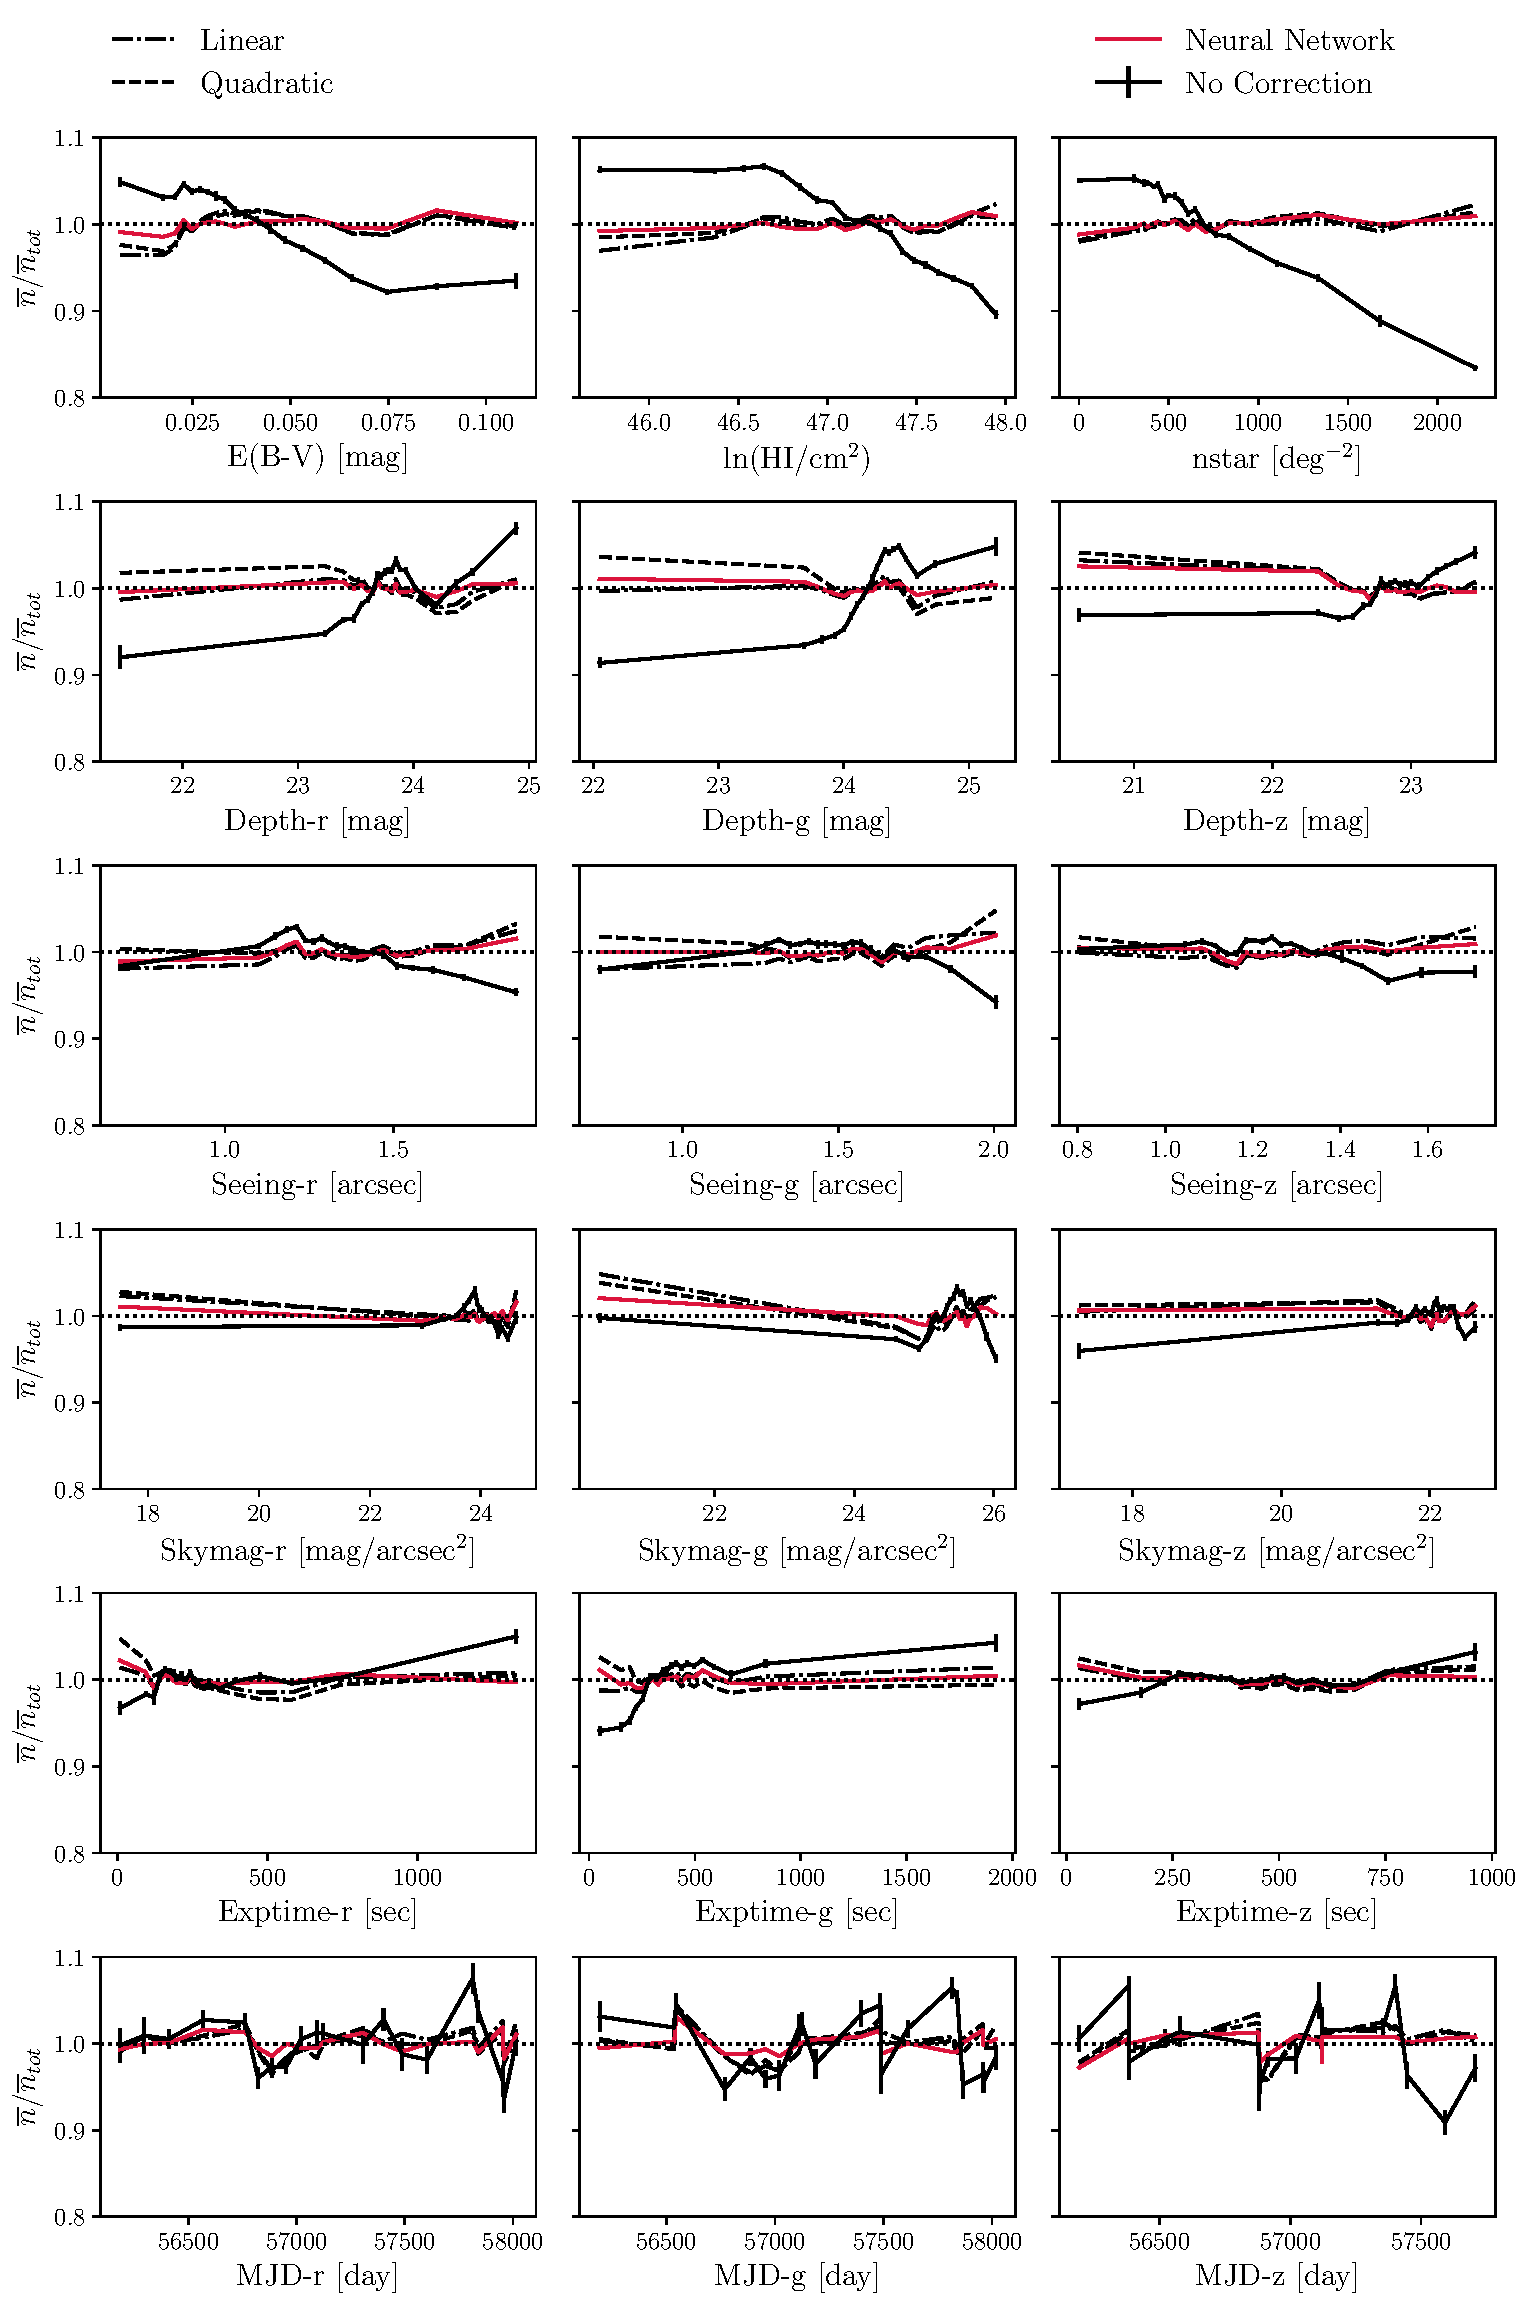
\includegraphics[width=0.8\textwidth]{nnbar_dr7.pdf}
\caption{The number density of galaxies as a function of the potential systematics. The solid black curve shows the result before mitigation (\textit{no correction}); the solid red curve is for the result after correcting with the neural network selection mask; the dot-dashed and dashed black curves represent mitigations with the linear and quadratic polynomial selection masks, respectively. The error bars are estimated using the Jackknife resampling of 20 non-contiguous subsamples of pixels within each imaging attribute bin (a total of 20 bins per attribute) and are shown only for one case. This plot again shows that the Galactic foregrounds such as the stellar density introduce a systematic trend in the galaxy density, which indicates a significant contamination by our own galaxy before mitigation. Such systematic trends are mostly removed with any of the three mitigation methods. \label{fig:nnbar}}
\end{figure*}



We next evaluate the performance of different mitigation techniques using the two-point statistics. We first show the cross power spectra between the DR7 observed galaxy density and various imaging attributes in the form of  $[\hat{C}^{g,s_k}_{\ell}]^2/\hat{C}^{s_k,s_k}_{\ell}$ in Fig. \ref{fig:clcross}. Again, this quantity approximately represents the level of contamination from each attribute to the auto power spectrum of galaxy density and we therefore compare this with the uncertainty in the auto power spectrum of galaxies (gray shades). Similarly, we plot $[\omega^{g,s_k}(\theta)]^2/\omega^{s_k,s_k}(\theta)$ in Fig.~\ref{fig:xicross} to assess the contamination in the auto correlation function. Fig. \ref{fig:clcross} and \ref{fig:xicross} show significant contamination on large scales from $ebv$, $lnHI$, and $nstar$ compared to the statistical fluctuation estimated from the Jackknife subsampling of the data. The stellar density map shows the highest cross power spectrum with the galaxy density map, which is in agreement with the previous results. Qualitatively, all three mitigation techniques perform well and substantially reduce the cross power below $\ell \sim 30$ and over all separation scales in the cross correlation function. The neural network method shows a slightly lower cross-power, but this appears to be merely related to the lower amplitude of the corresponding auto galaxy power spectrum compared to the other two cases. We note the spurious peak in the cross correlation against exptime-z in Fig.~\ref{fig:xicross} near the expected angular location of the BAO feature and such feature necessitates thorough investigations of imaging systematics in analyzing the auto clustering statistics of the spectroscopic data for BAO analysis.\\

\begin{figure*}
\centering
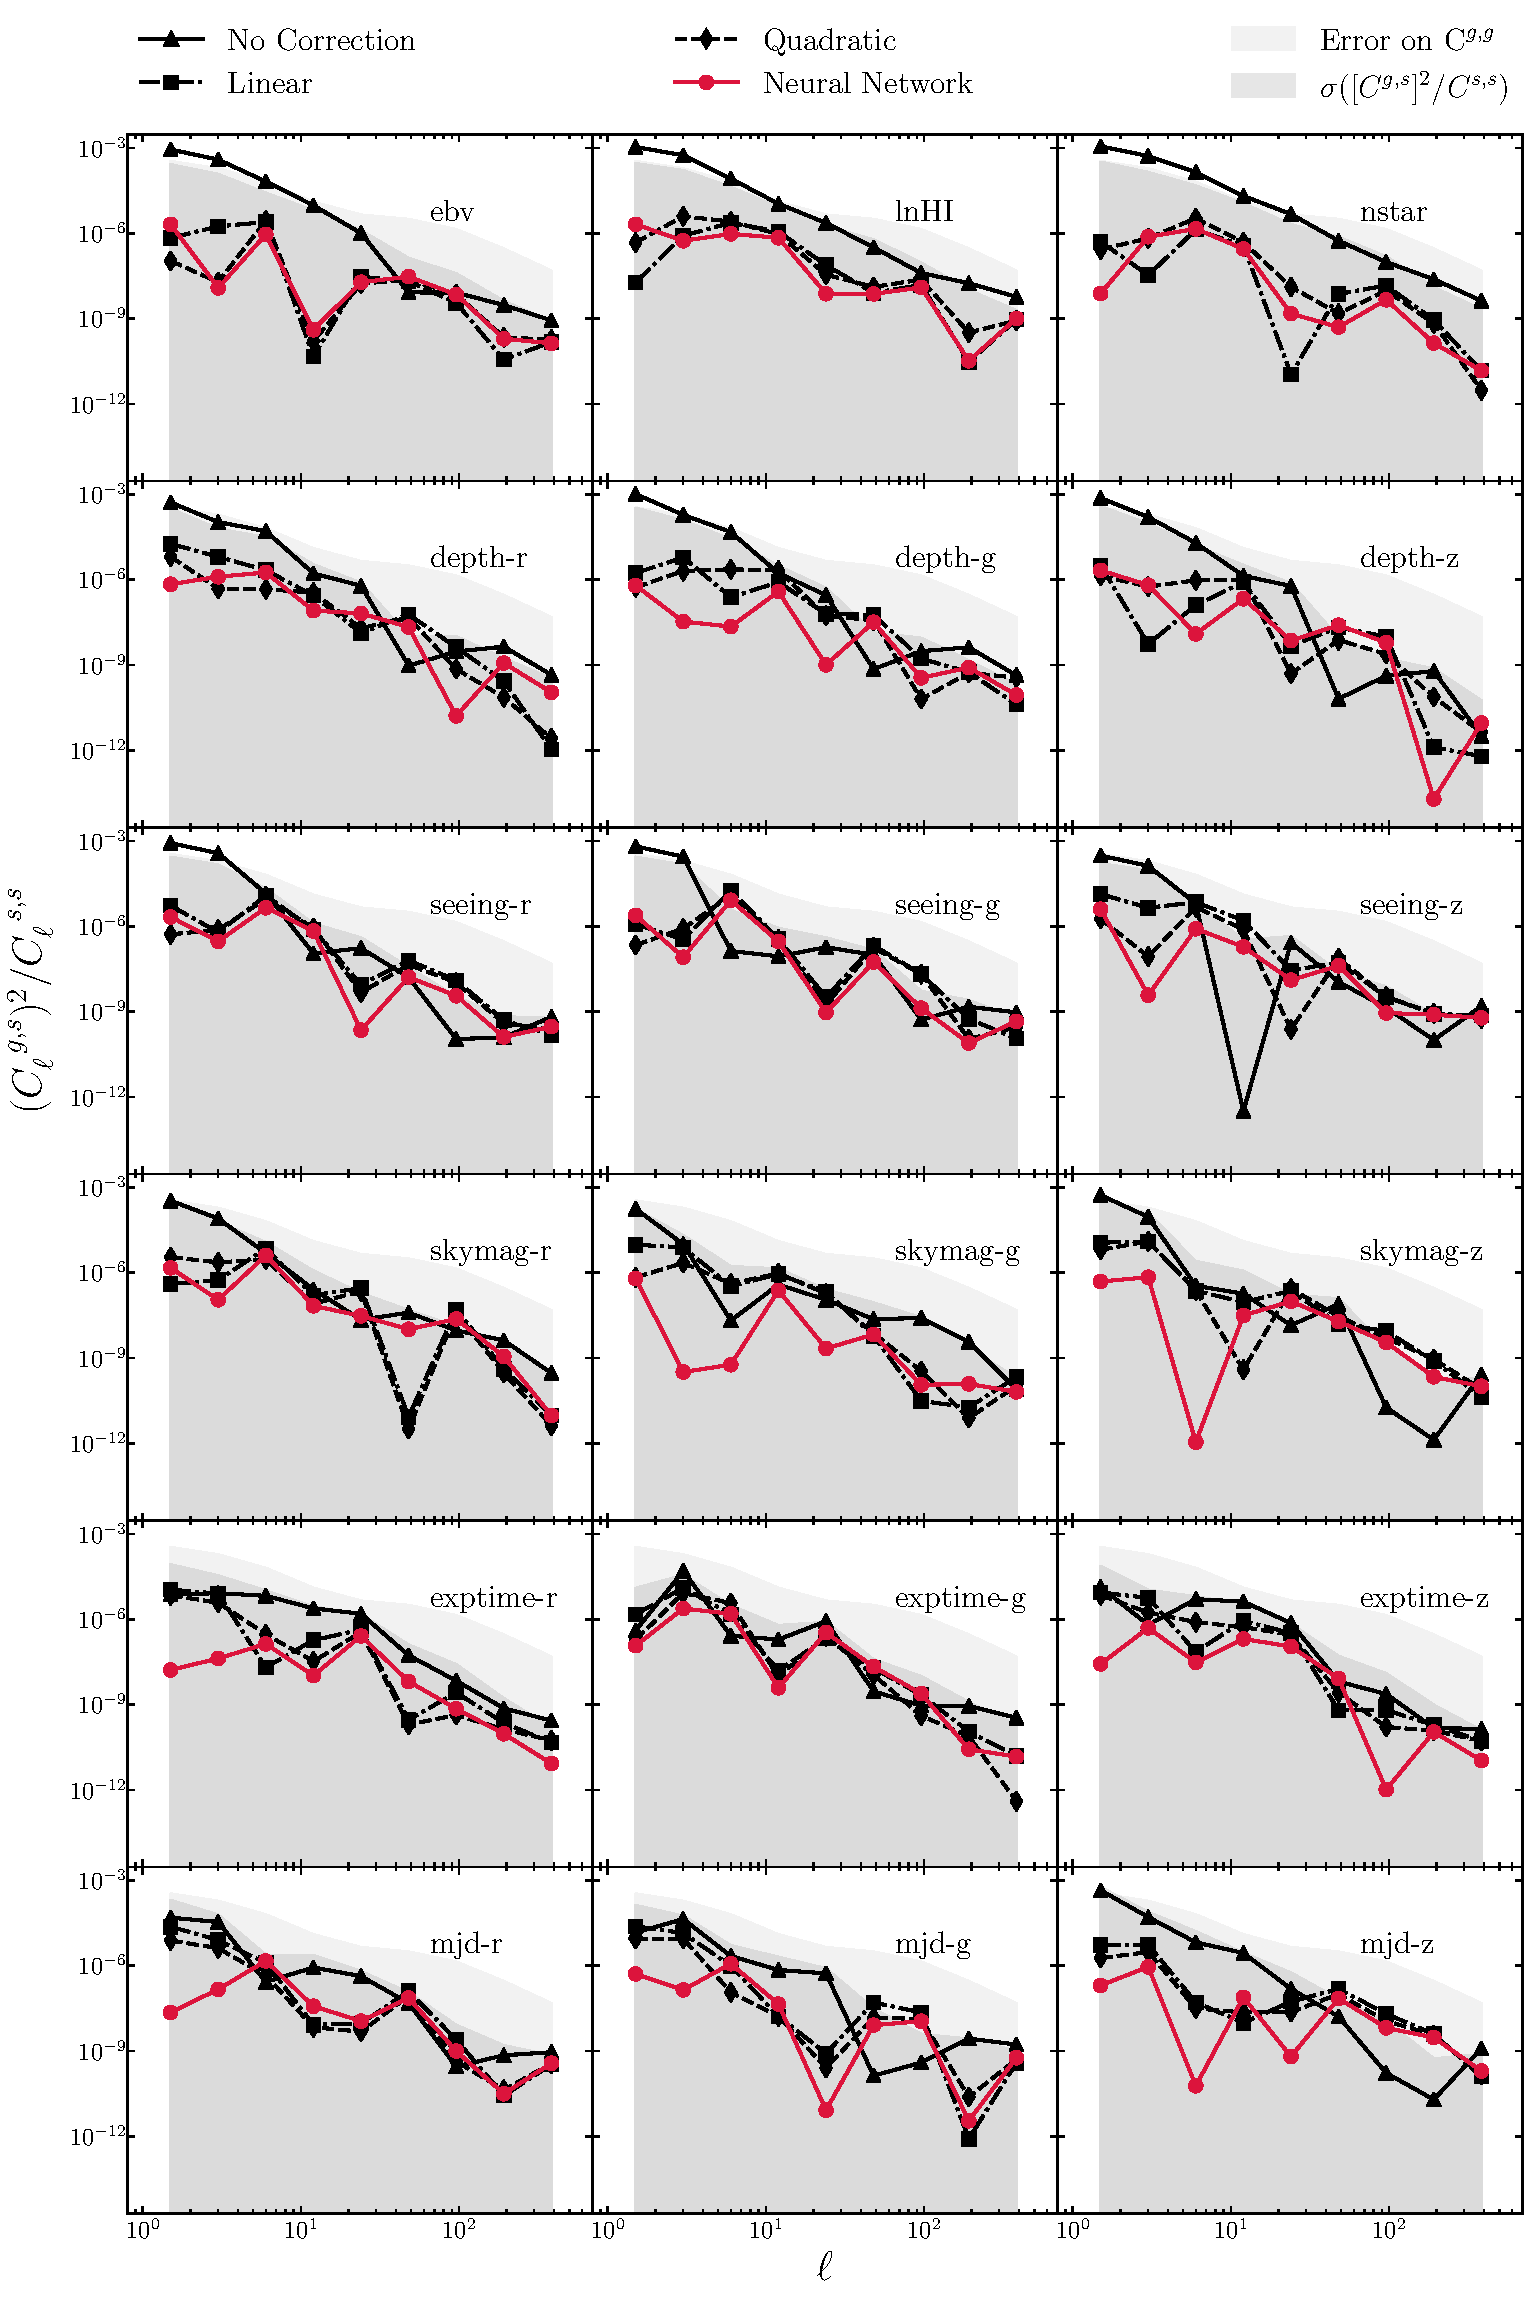
\includegraphics[width=0.8\textwidth]{dr7_crosscl.pdf}
\caption{The cross power spectrum $\hat{C}^{g,s_k}_{\ell}$ between the DR7 observed galaxy density and the imaging attributes $s_k$ normalized by the auto power spectrum of the imaging attribute $\hat{C}^{s_k,s_k}_{\ell}$. The plotted quantity $[\hat{C}^{g,s_k}_{\ell}]^2/\hat{C}^{s_k,s_k}_{\ell}$ approximately represents the level of contamination to the auto power spectrum of the galaxy density $\hat{C}^{g,g}_{\ell}$.  The grey shaded region shows the Jackknife error estimate of $\hat{C}^{g,g}_{\ell}$. The black solid curve shows the result before mitigation (\textit{no correction}), while the solid red curve shows the result after correcting for the systematics with the neural network selection mask. The dot-dashed and dashed black curves show the corrected results with the linear and quadratic polynomial model selection masks, respectively. \label{fig:clcross}}
\end{figure*}


We finally present the effect of the imaging attributes before and after mitigation on the auto galaxy clustering statistics. In Fig. \ref{fig:clxi}, we illustrate the measured two-point clustering statistics for the DR7 data set: the measured angular power spectrum without shot-noise subtraction is shown in the left panel, and the HEALPIX-based angular correlation function is shown in the right panel. The solid black curve shows the measured clustering before mitigation, while the corrected measurements using the traditional linear, quadratic polynomial, and the default neural network models are shown respectively with the black dot-dashed, black dashed, and solid red curves. The dotted curves in both panels are a redshift-space linear theory prediction with galaxy bias of 2 using the surface density $n(z)$ of NGC eBOSS ELG ~\citep[Tab. 4 of][]{Raichoor2017MNRAS.471.3955R} and assuming the fiducial cosmology of \citet{ross2011ameliorating,2012ApJ...761...14H} with shot noise, while we did not include the survey window effect. In the right panel, the linear and the quadratic polynomial mitigation results are indistinguishable and overlaid.\\ 

The comparison between the clustering before correction (solid black curves) and the fiducial linear theory prediction (dotted curves) suggests that the imaging systematics affect the clustering measurements mostly on large scales, e.g., large separation angles or small multipoles, as expected~\citep[see e.g.,][]{myers2007clustering, ross2007higher, huterer2013calibration}. We find that all the mitigation methods are able to reduce such large scale contamination, while there still remains substantial excess clustering on large scales with the two traditional linear multivariate methods. The neural network method is much more efficient in reducing such excess. In comparison to our default neural network model, we also show the neural network model without the feature selection process labeled as `plain' (blue dashed curves), which is very similar to the default case. Although we do not know the true underlying clustering for the real survey, the typical linear theory prediction shows a downturn of power for $\ell<30$ and redshift-space distortions tend to increase the power on this scale, making the power spectrum almost flat for $\ell<30$ as shown with the dotted curve in the left panel. Note that our default neural network method best returns the expected behavior on this scale. For $\ell << 10$, we expect the survey window function would become more important. In the next section, we test the mitigation methods using the mock datasets for which we know the true clustering signals. As will be demonstrated, our default neural network model with the feature selection process is chosen based on this mock test. \\

\begin{figure*}
\centering
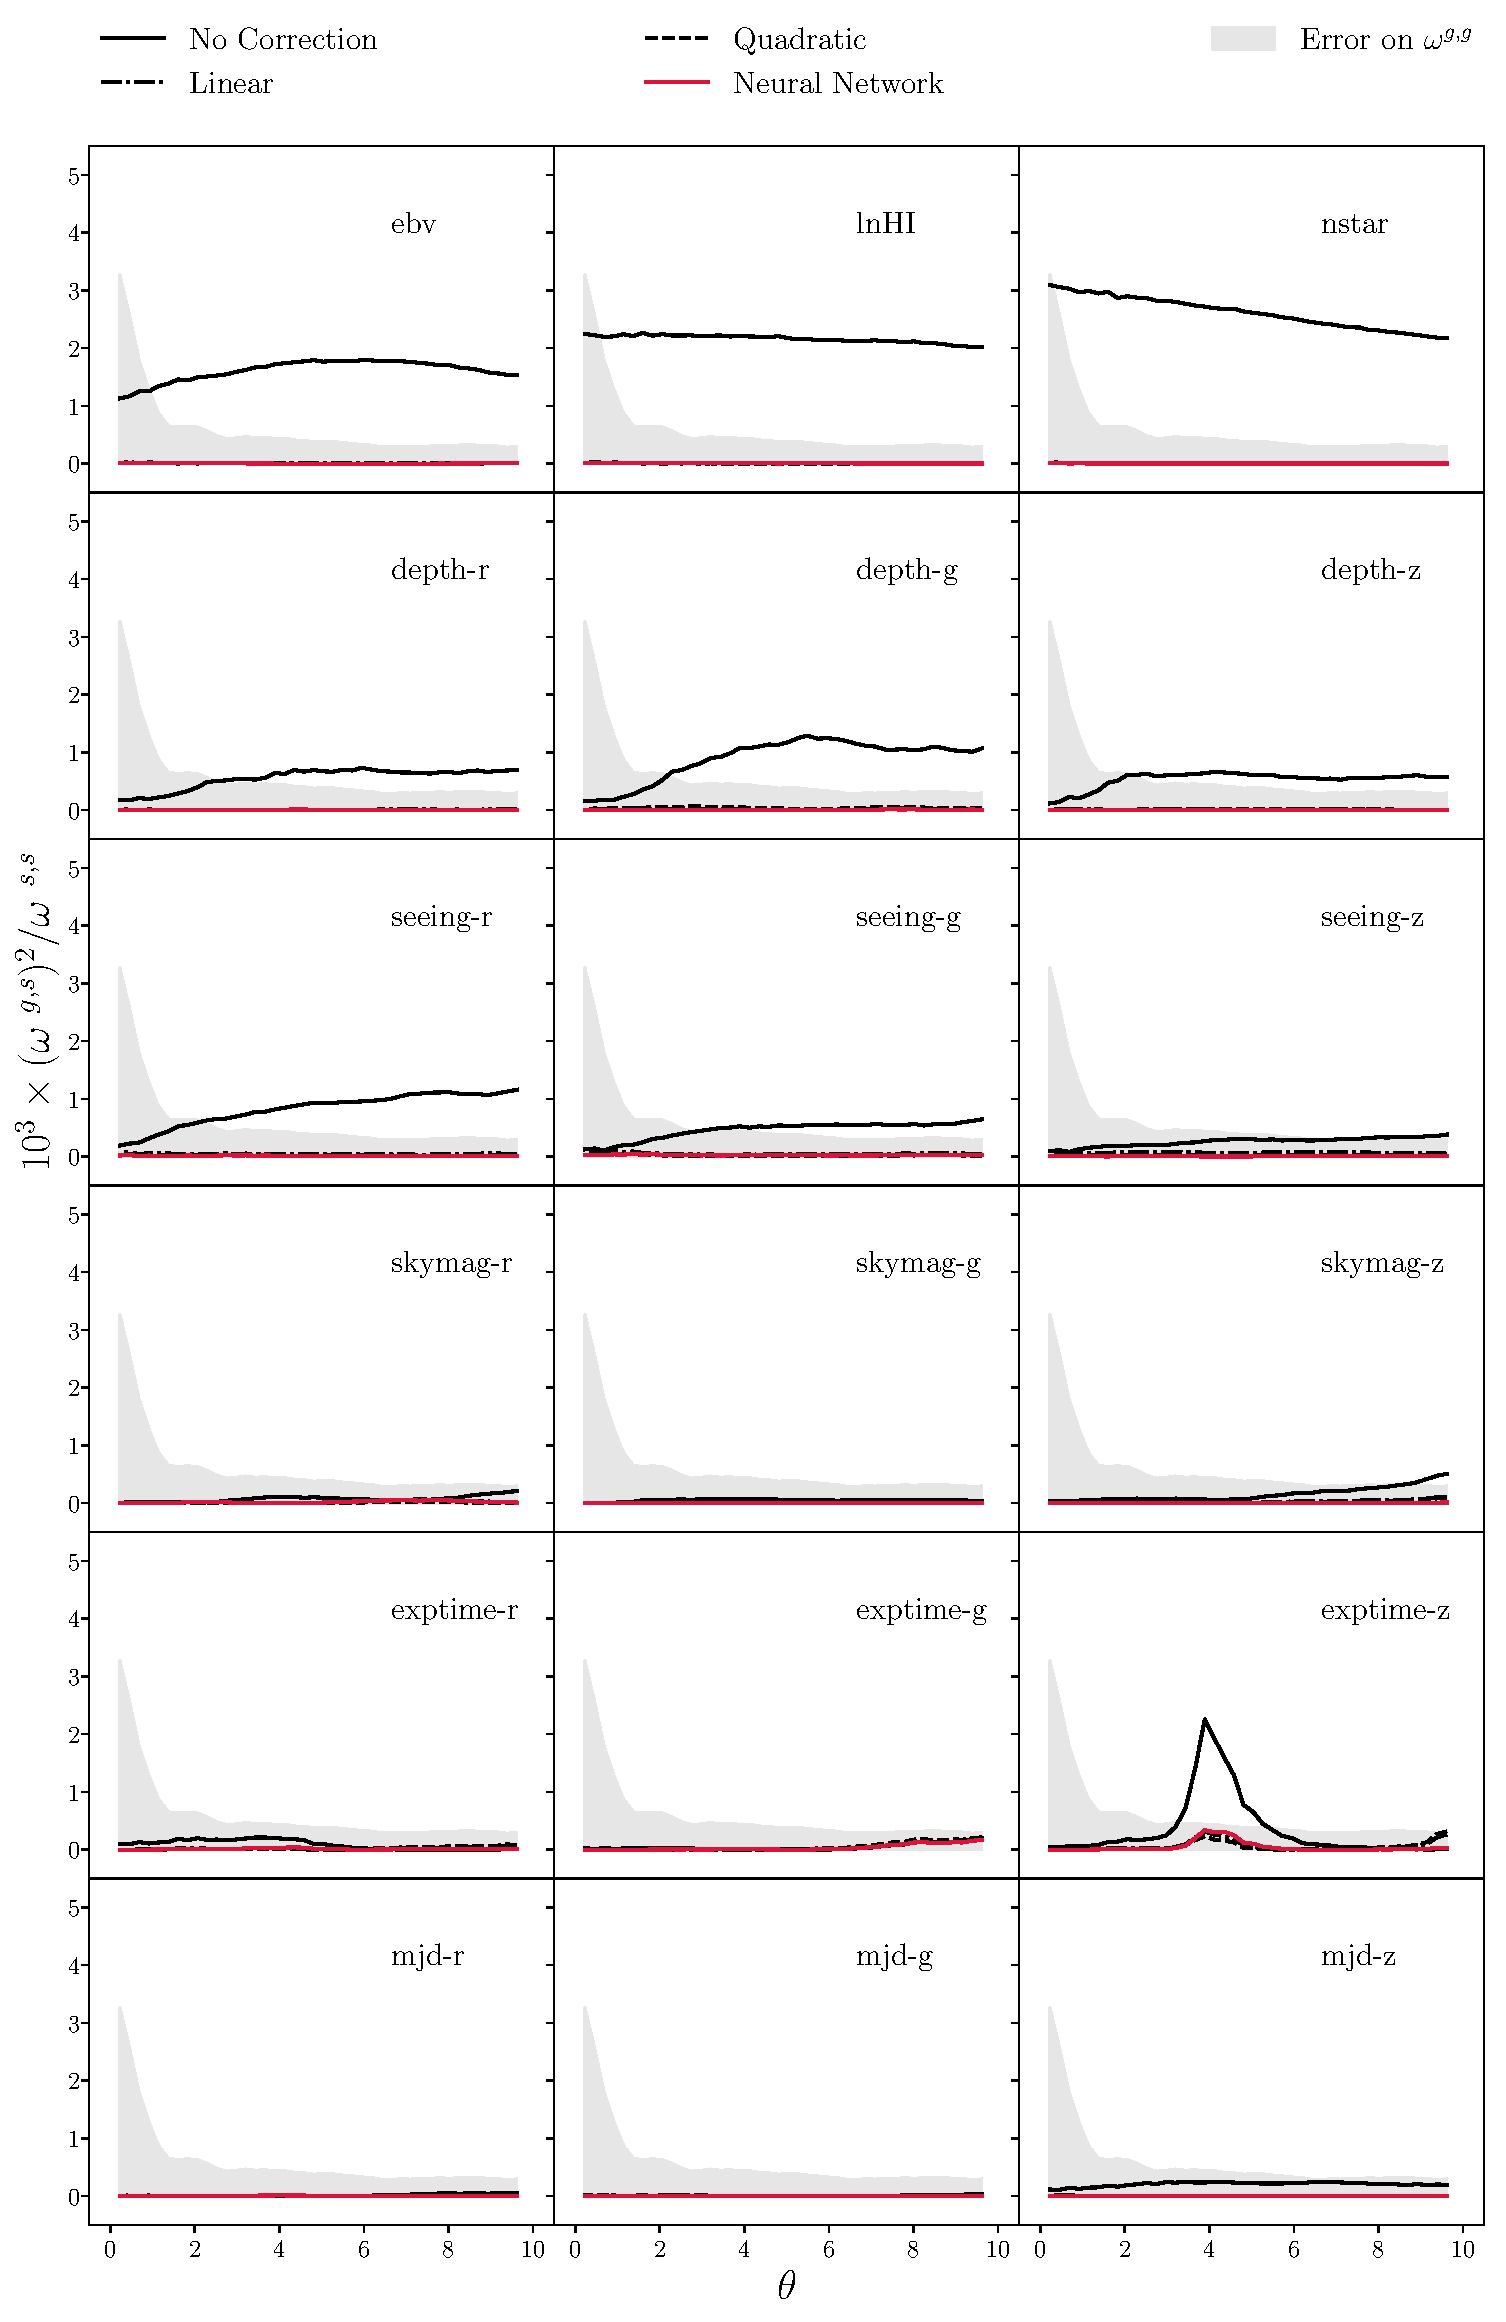
\includegraphics[width=0.8\textwidth]{dr7_crossxi.pdf}
\caption{The cross correlation function $\omega^{g,s_k}(\theta)$ between the DR7 observed galaxy density and the imaging attributes $s_k$ normalized by the auto correlation function of the imaging attribute $\omega^{s_k,s_k}(\theta)$. The plotted quantity $[\omega^{g,s_k}(\theta)]^2/\omega^{s_k,s_k}(\theta)$ approximately represents the level of contamination to the auto correlation function of the galaxy density $\omega^{g,g}(\theta)$.  The grey shaded region shows the Jackknife error estimate of $\omega^{g,g}(\theta)$. All mitigation techniques are able to reduce the excess clustering singla which is due to the imaging systematics.  \label{fig:xicross}}
\end{figure*}

\begin{figure*}
\centering
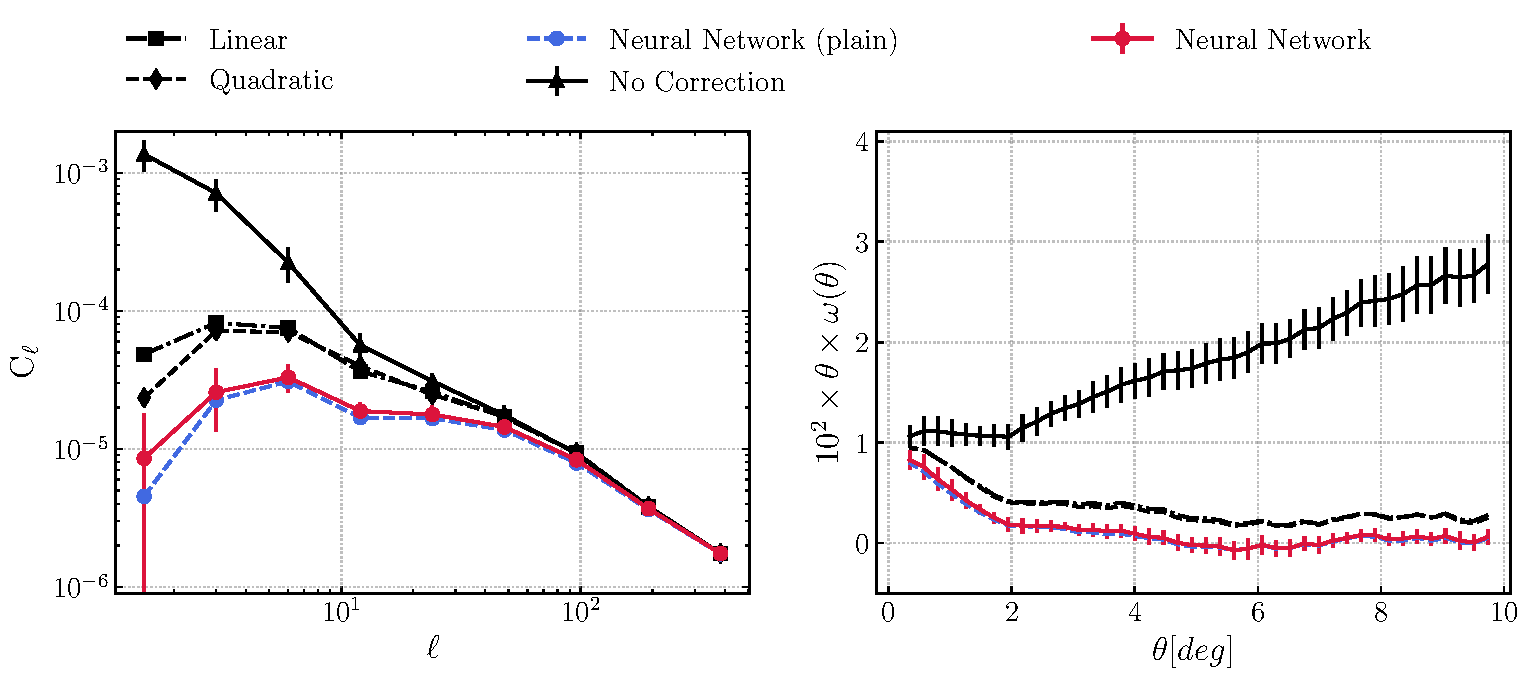
\includegraphics[width=\textwidth]{dr7_clustering.pdf}
\caption{Two-point clustering statistics for the DECaLS DR7 dataset. \textit{Left}: the measured angular power spectrum without shot-noise subtraction. \textit{Right}: the HEALPIX-based angular correlation function. Solid black curves show the measured statistics without correcting for the systematic effects (\textit{no correction}). The dashed and dot-dashed black curves show the statistics after correcting with linear and quadratic polynomial mitigation methods, respectively. The solid red curves show the results after correcting with our default neural network method. The dashed blue curves show the results with the neural network method but without the feature selection process. The dotted curves in both panels are a redshift-space linear theory prediction using $galaxy\;bias = 2$ and the surface density $n(z)$ of NGC eBOSS ELG ~\citep[Tab. 4 of][]{Raichoor2017MNRAS.471.3955R} and assuming the fiducial cosmology of \citet{ashley2012MNRAS,2012ApJ...761...14H}. In the left panel, while the data includes the survey window function effect, the theory model does not include the survey window effect. The estimated shot noise was added to the theory model in the left panel. The errors are estimated using the Jackknife resampling with 20 contiguous sub-regions.} \label{fig:clxi}
\end{figure*}

\subsection{Testing the mitigation methods on the mock data}
We treat the mocks as if the contamination model was unknown and apply the mitigation pipeline on the mocks as exactly used for the real dataset. After modeling the selection mask for each mock, we remove the pixels whose selection masks values are < 0.5 or > 2.0. This reduces the mock footprint size from 86875 to 86867 pixels. Again, the mocks do not include the redshift-space distortions.

\subsubsection{Feature selection of mock galaxies}
Fig.~\ref{fig:mockablation} shows the distribution of the imaging attributes selected by the feature selection process for all five partitions of 100 null (left) and contaminated (right) mocks. For the null mocks, there is no contamination and the feature selection correctly removes most or all imaging attributes, as demonstrated by the sparse distribution of the points in the left figure. The imaging attributes that survived feature selection, probably due to a coincidental correlation with the galaxy density, are randomly distributed. On the other hand, the right panel shows that the feature selection procedure correctly identifies most of the input contamination attributes (the solid horizontal lines) for the contaminated mocks and almost always selects $lnHI$ and $nstar$. Indeed, as shown in Fig.~\ref{fig:dr7ablation}, these two attributes were the two most significant input contamination.


\subsubsection{Mean mock galaxy density}
In Fig.~\ref{fig:nnbarmock} we show the number density of mock galaxies, averaged over 100 mocks, as a function of the imaging attributes. As expected, the galaxy density of the contaminated mocks show strong or moderate dependence on $ebv$, $nstar$, $lnHI$, $seeing-g$, $skymag-g$, $skymag-z$, $exptime-r$, $exptime-z$, $mjd-g$, and $mjd-z$ which were indeed the inputs to the contamination model. Meanwhile, the galaxy density also shows strong dependencies on $mjd-r$, $depth-r$, $depth-g$, and $depth-z$ through the correlation between these and the input contamination attributes. Looking at this result alone from a real data perspective, one would not be able to single out the underlying imaging attributes that are directly responsible for the contamination. When the inputs to the mitigation procedure include all contamination input maps, Fig.~\ref{fig:nnbarmock} shows that all methods effectively remove the dependence.\\
 

 
\subsubsection{Angular power spectrum of mock galaxies}
Fig. \ref{fig:deltaclmock} shows the mean angular power spectrum of 100 null and 100 contaminated mocks in the left and right panel, respectively, in the top row. In the middle row, we illustrate the remaining bias on clustering after mitigation as an offset from the true power spectrum (i.e., the null power spectrum from the left panel). To account for the increased shot noise during contamination, we removed the same constant power from all contaminated/mitigated power spectra in the right panel until their small scale power matches that of the null mock power spectrum. One can see that the contamination substantially increased power at $\ell < 50$.\\

Since the contamination model is based on the linear polynomial model, all three fitting methods, i.e., the linear, quadratic, and neural network, are capable of reproducing the true input contamination, while they perform differently in the presence of the two layers of noise we added and the eight additional imaging attributes that are nontrivially correlated with the ten contamination input attributes. In the right top and middle panel, we find all three methods effectively remove the contamination over $\ell <100$; in detail, the linear (black dot-dashed) and the quadratic polynomial (black dashed) methods slightly over-correct power while the neural network method (solid red) slightly under-corrects it. Note that, without the feature selection process (dashed blue), the neural network method would also over-correct the large scale power like the linear and quadratic polynomial models.\\

The remaining bias can be compared to the typical error expected for such data. The dark and light grey shaded regions in middle panels indicate the 1-$\sigma$ confidence regions for the mean and the individual mock of the 100 mocks, respectively.  We quantify the significance of such remaining bias by calculating $\chi^2$, the sum of the squared offset weighted with the diagonal variance for the mean at each $\ell$ bin. Note that we use the variance from the 100 null mocks for calculating $\chi^2$ of the contaminated mocks in order to avoid an advantage of increased variance after contamination. We find the neural network method returning $\chi^2=15.4$ from six $\ell$ bins within $10<\ell <200$, while the linear polynomial mitigation returns 27.5. While the neural network model appears to perform the best, the difference in $\chi^2$ among different mitigation methods is not significant compared to the $\chi^2=17643$ before mitigation. 
 Such $\chi^2$ can depend on the lower limit of $\ell$ we consider. In Fig. \ref{fig:chi2clmock}, we investigate the behavior of the remaining bias depending on $\ell_{min}$, which shows that the neural network method consistently returns a lower remaining bias for various $\ell_{\rm min}$ choices. However, for the contaminated mocks, the difference is small and we conclude that all mitigation methods perform similarly well for the contaminated mocks. \\

The bottom panels of Fig.~\ref{fig:deltaclmock} compare the noise introduced by the three different mitigation processes. The right panel shows that the contamination process (solid black) introduces additional noise on large scales relative to the variance of the null mocks (the gray shade). After mitigation, the variance is reduced, which is probably related to the decrease in the large scale power, since the variance of power is proportional to the amplitude of power itself in the Gaussian limit. The quadratic method shows the smallest fractional error on large scales due to the reduced amplitude after correction. In all cases, if we calculate the fractional variance with respect to the measured $C_\ell$ (e.g., $\sigma C_{\ell, NN}/C_{\ell, NN}$ instead of  $\sigma C_{\ell, NN}/C_{\ell, Null}$), it agrees with the fractional variance of the null mock (gray shade). Therefore, we do not observe a nontrivial increase in variance by any of the mitigation methods we tested. \\

The left panel of Fig.~\ref{fig:deltaclmock} shows that, in the absence of contamination, both the linear and quadratic polynomial methods over-correct the large scale power since the fitting methods can always find purely coincidental consistency between the imaging attributes and the cosmic variance. The quadratic method that has a greater freedom appears more prone to such problem. The neural network method without the feature selection process shows a lesser degree of overfitting than the linear methods, probably due to the validation procedure. The figure shows that our default neural network method, i.e., with the feature selection procedure that selects the dominant imaging attributes and reduces the dimension of the input features, is the most robust mitigation methodology against overfitting.


\subsubsection{Cross power spectrum of mock galaxies and imaging attributes}
In Fig. \ref{fig:clcrossmock}, we show the cross power spectrum of the mock catalogs and the imaging attributes for different mitigation techniques. Again, the dark and light shaded region show the 1$-\sigma$ confidence region of the mean of the mocks and each mock, respectively. All three methods substantially reduce the cross power with the imaging attributes. The neural network method tends to show a small residual for $\ell <10$ that is greater those of the linear and quadratic polynomial models. This is partly due to the greater auto galaxy power spectrum amplitude (in Fig.~\ref{fig:deltaclmock}) after mitigation than those by the other methods. Meanwhile we still find residual correlation with skymag-z and mjd-z even after accounting for the effect of the auto power spectrum amplitude. Without the feature selection procedure (dashed blue), the neural network also returns smaller residual. In essence, we see that once feature selection is applied, the neural network only corrects to a certain level, controlled by the specifics of the feature selection procedure. This protects against over-fitting due to random correlations between the imaging attributes and the galaxy density field.\\ 

As a sanity check, if we use the true input linear contamination model to mitigate the systematics (purple dot-dashed line), the cross-correlation completely vanishes as expected. For the null mocks, all mitigation methods return negligible cross-correlation. Overall, while the cross-correlation statistics between the galaxy density and the systematics attributes are a useful indicator for the level of contamination, we find it may be difficult to infer and discriminate the level of contamination in the density field from such cross correlation statistics beyond what can be probed by the auto power spectrum.

\subsubsection{A case with underfitting}
It is possible that we may identify only a subset of the contamination attributes for a given data set and attempt to mitigate the contamination based on such limited information. We consider a situation where we input only five imaging attributes to the mitigation procedure: four from the true contamination inputs, i.e., $EBV$, $lnHI$, $nstar$, $skymag-g$ and one that is not among the true contamination inputs, but correlated with the contamination inputs, i.e., $depth-r$. The neural network method could be more resilient to such limited information since its nonlinear activation function may allow the mitigation procedure to better utilize the correlation between different input imaging attributes. In Fig.~\ref{fig:mockdclextra}, the linear polynomial method with `few' inputs shows a lesser degree of overfitting for the null mocks, compared to the default linear case, while showing under-fitting for the contaminated mocks. This is expected as the freedom of the linear model is now limited.  The neural network method with the `few' inputs (without feature selection) returns a very similar pattern as the linear `few' case, which implies that our current default neural network method does not have an advantage over the linear model in such case despite its greater flexibility. This underfitting case may be worth future investigation, as apparent excess clustering remains in the DECaLS DR7 data in Fig.~\ref{fig:clxi} when any method is applied, but especially in the case of the application of multivariate linear models.

\subsubsection{Summary}
In summary, we find that our default neural network method is more robust against overfitting based on the test with the null mocks. This appears to be mainly due to the feature selection process that appropriately reduces the flexibility of mitigation. Based on the tests with the contaminated mocks, we find that both the linear and neural network methods perform equally well in terms of the residual bias, while the neural network method is more robust against overfitting. The quadratic polynomial method appears to be more prone to the overfitting problem than the other two methods since it has a greater flexibility than the input contamination model, but without a way to suppress the flexibility. All methods do not increase fractional variance during the mitigation process. Note again that we deliberately choose the linear model in contaminating the mocks in this test in order to prevent a disadvantage in using the linear and quadratic polynomial methods.  Therefore, the decent performance of the linear method is warranted. In real data, the contamination due to observational effects can take a more complex form as implied by the difference in the mitigation results between the data and our mocks. Therefore our mock test is a conservative estimation of the comparative mitigation capability of our default neural network method. 


\begin{figure*}
    \centering
    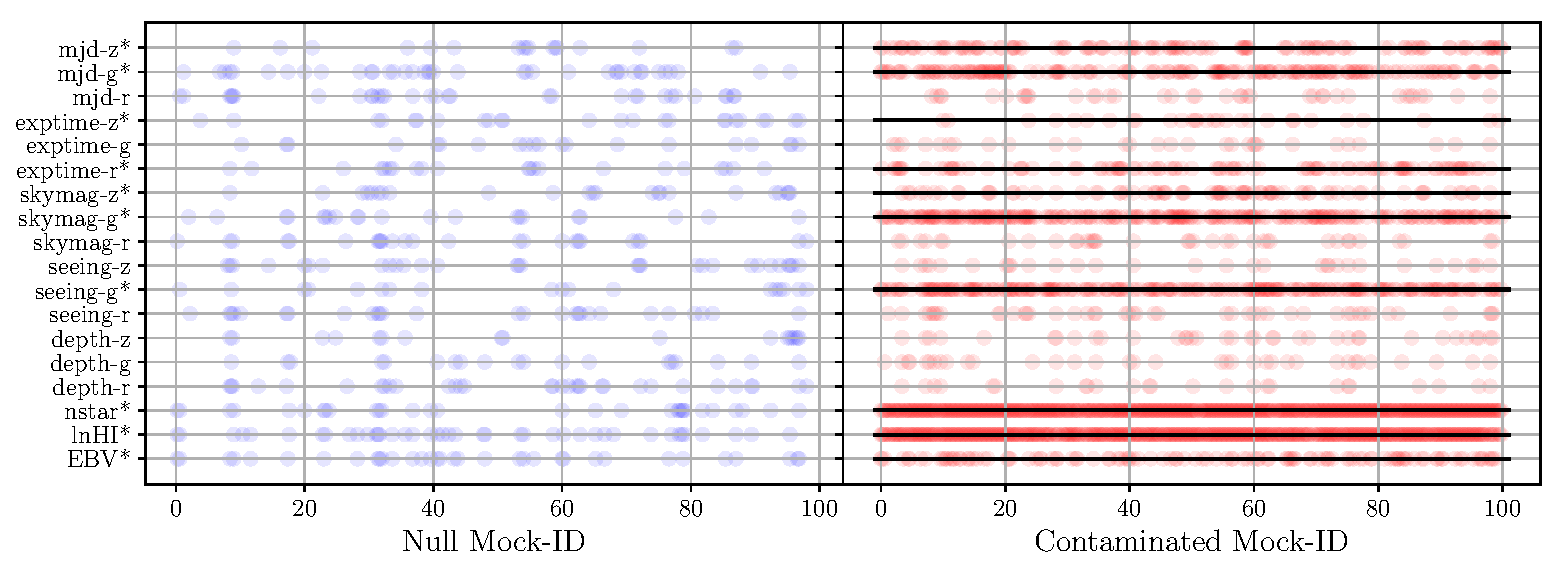
\includegraphics[width=0.95\textwidth]{hyper-params.pdf}
    \caption{Important imaging maps identified by the feature selection procedure for all five partitions of the 100 null (left) and contaminated mocks (right). The maps used in the input contamination model were marked by `*' and horizontal black solid curves. }
    \label{fig:mockablation}
\end{figure*}


\begin{figure*}
    \centering
    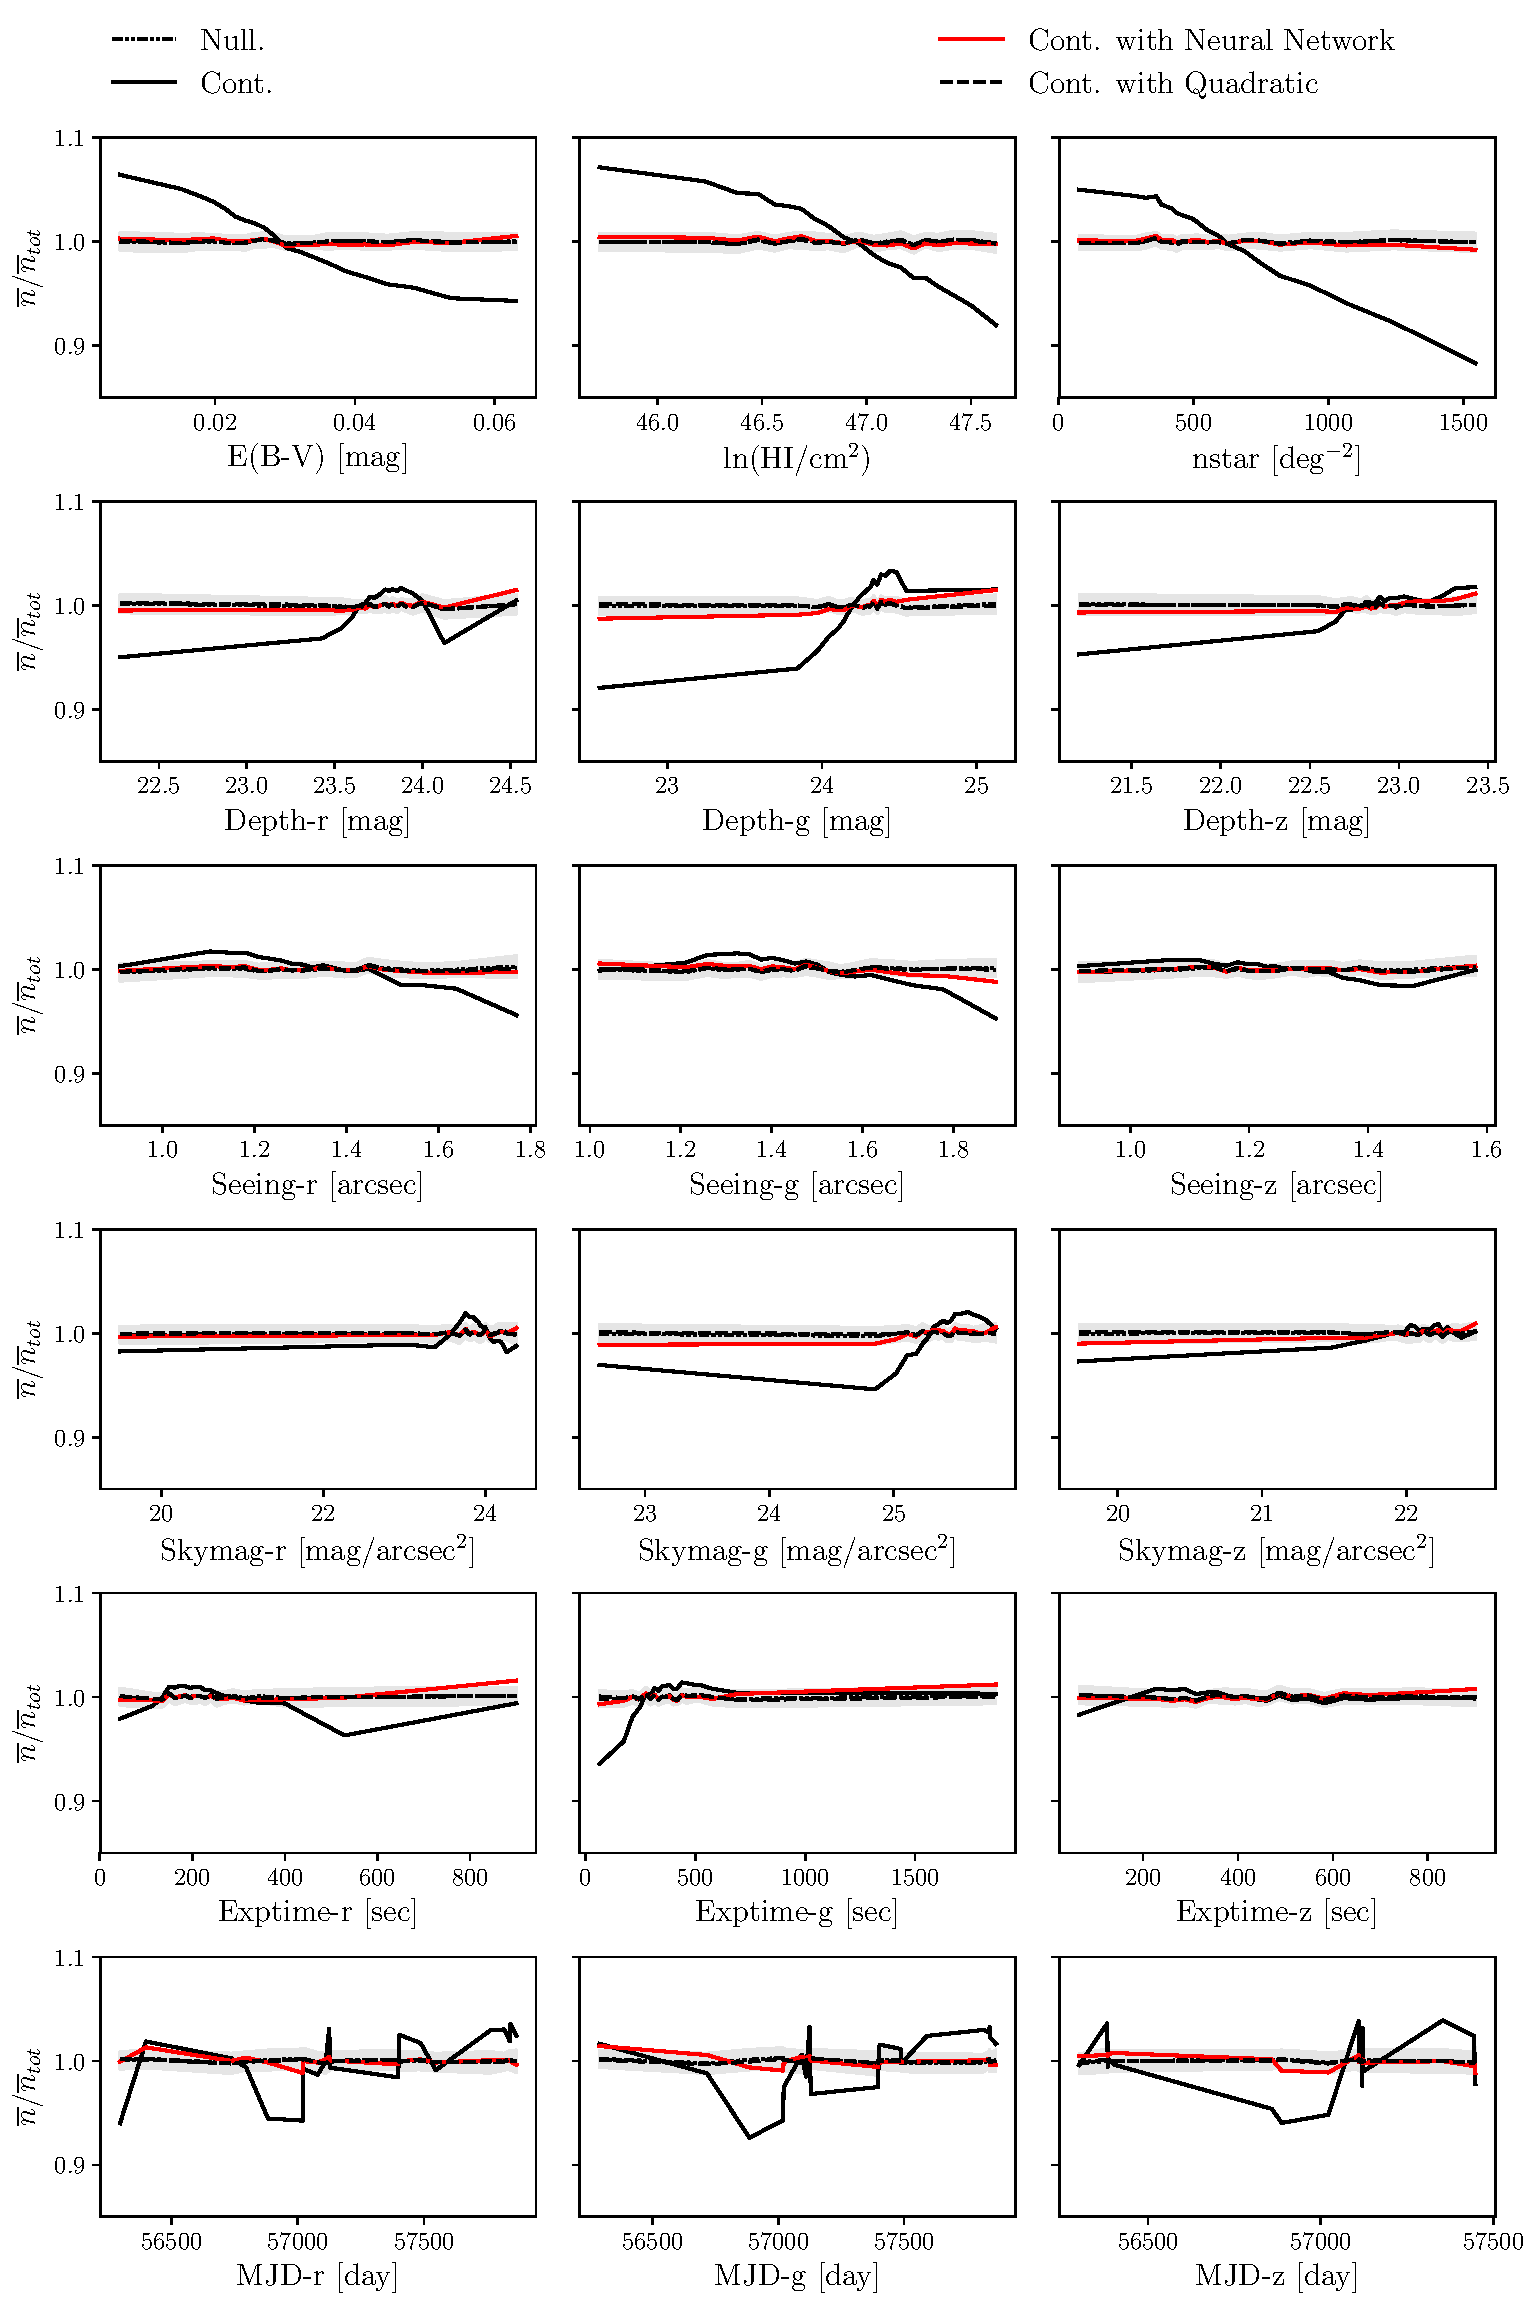
\includegraphics[width=0.8\textwidth]{nnbar_mocks.pdf}
    \caption{The number density of mock galaxies as a function of the potential systematics averaged over 100 mock datasets. The grey shaded region illustrates 1$-\sigma$ dispersion in the mocks. The black solid curve shows the mean density dependence on the imaging attributes for the contaminated mocks. The solid red curve shows the mean density after correcting for the systematics with the neural network selection mask. The dashed black curve shows the corrected results with the quadratic polynomial model selection mask. The result of the linear polynomial model is almost unity, and therefore is omitted for clarity.}
    \label{fig:nnbarmock}
\end{figure*}



\begin{figure*}
\centering
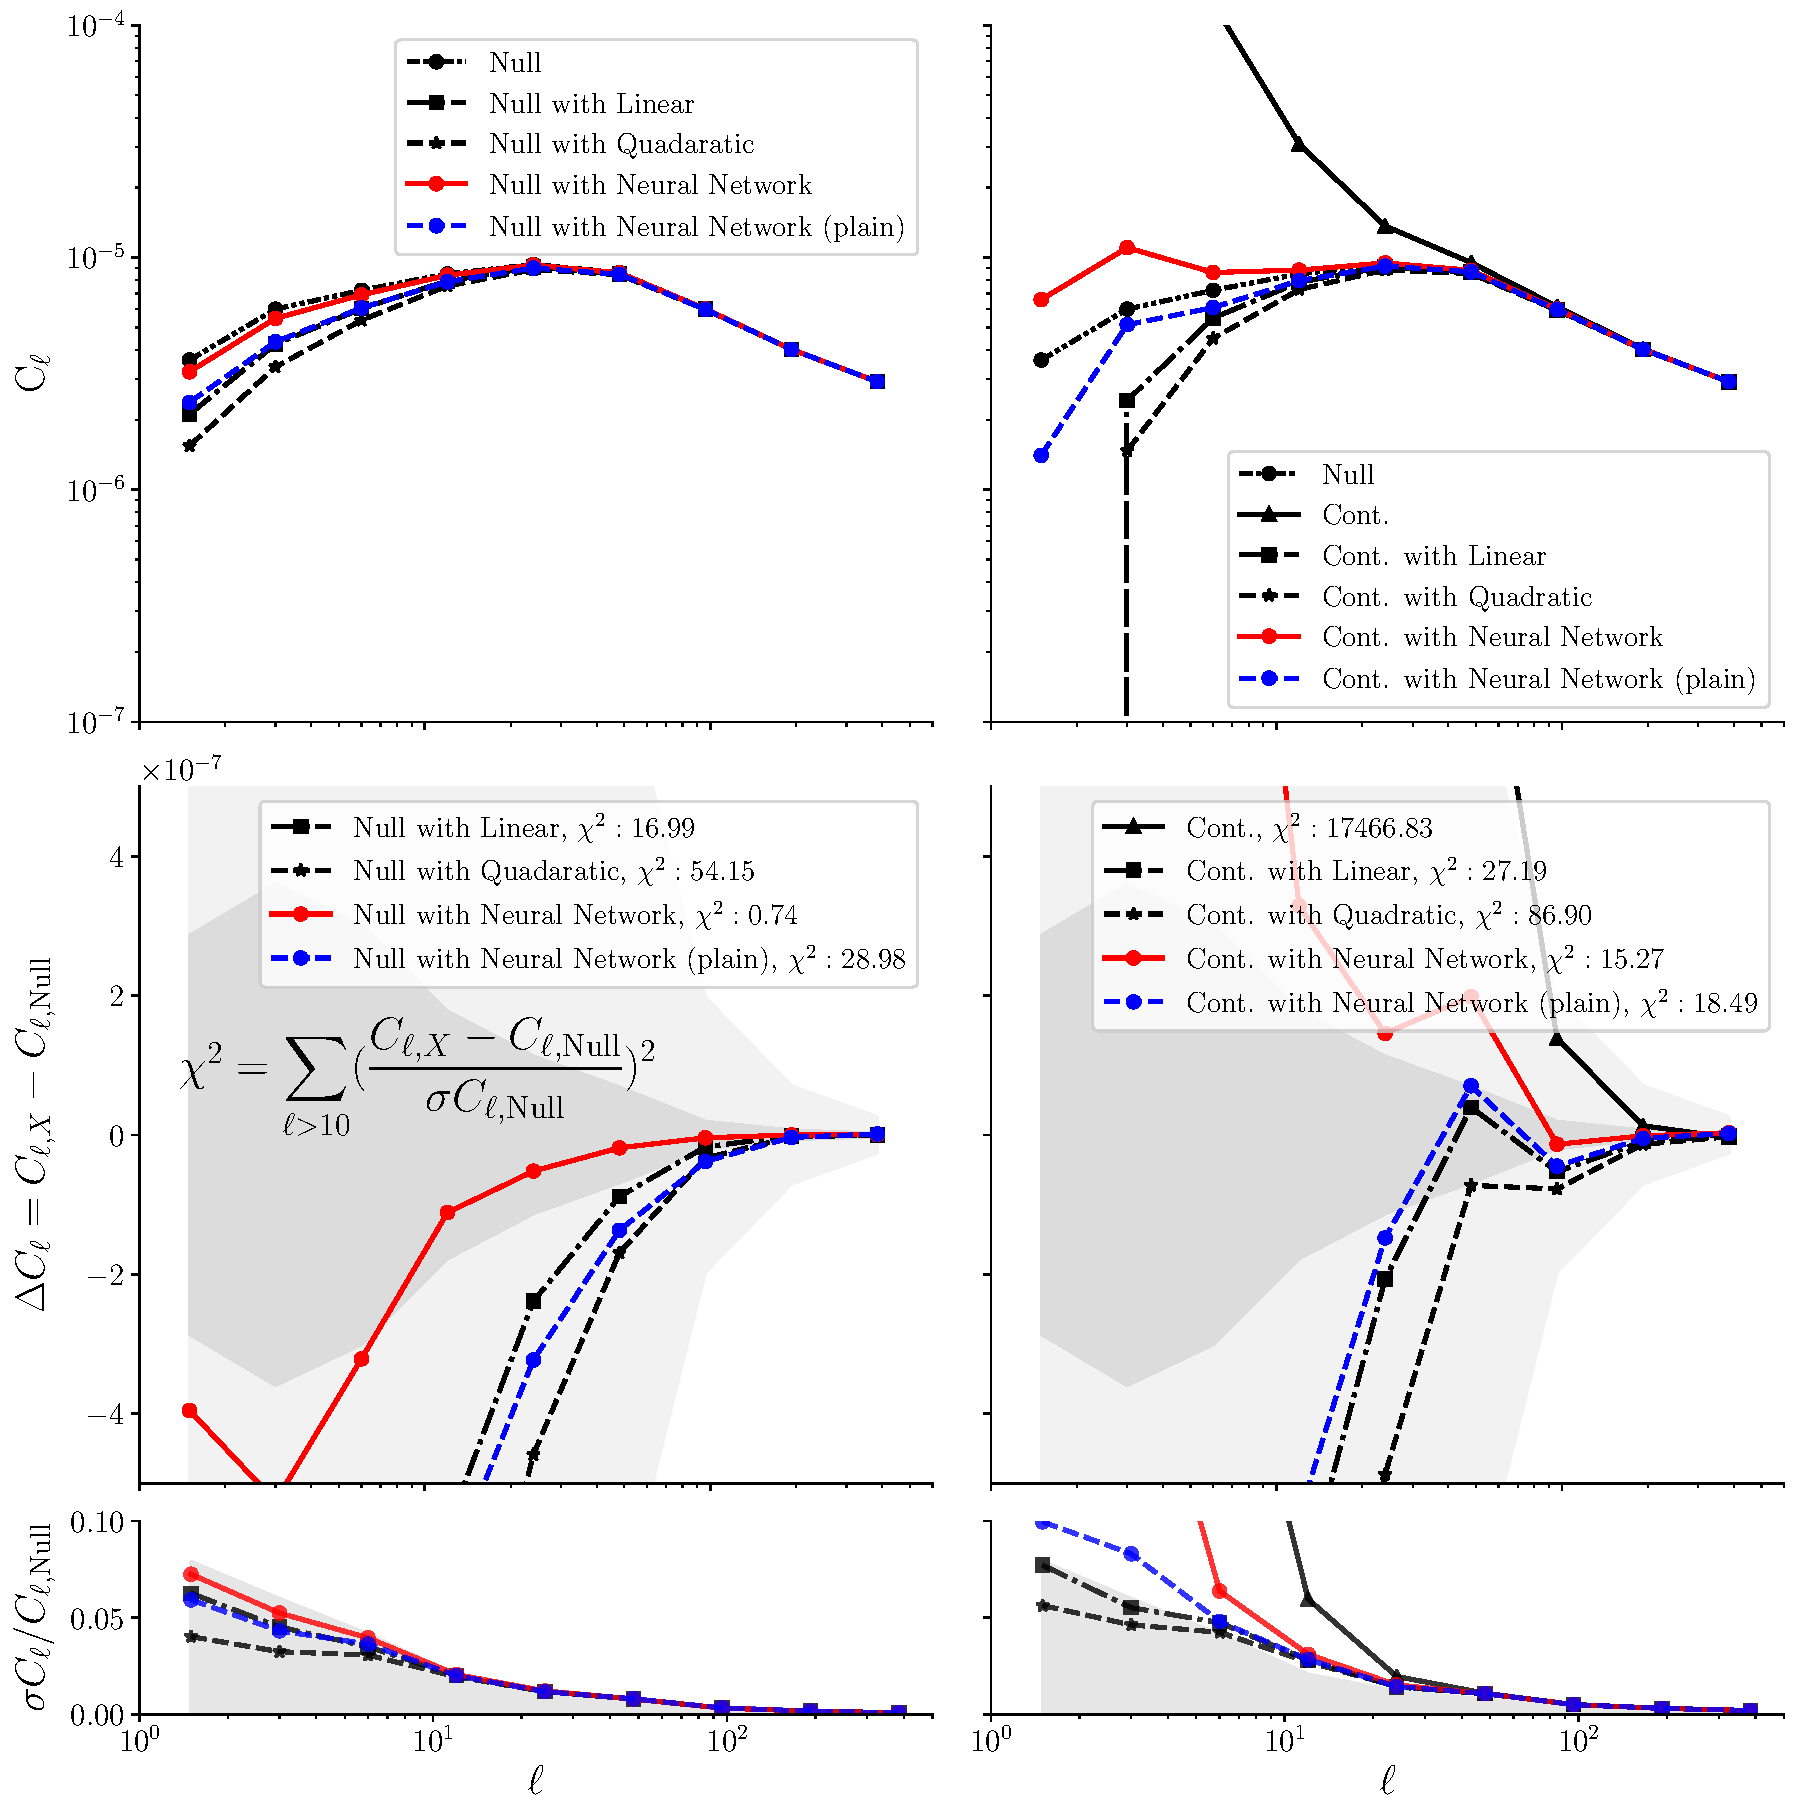
\includegraphics[width=0.7\textwidth]{mocks_deltacl.pdf}
\caption{\textit{Top row}: The angular power spectrum of the contaminated (null) mocks in the right (left) panels. \textit{Middle row}: The power spectrum subtracted by the mean of the null mocks to better visualize the remaining bias after each mitigation. The dark grey shaded region shows the 1$-\sigma$ confidence region of the mean of 100 mocks, while the light grey area shows the 1$-\sigma$ confidence region for one mock, calculated from the dispersion of 100 mocks. To account for the increased shot noise during contamination, we remove the same constant power from all contaminated/mitigated power spectra until their small scale power matches that of the null mock power spectrum. We quantify the significance of the remaining bias by calculating $\chi^2$, the sum of the squared offset weighted with the diagonal variance of the mean $C_\ell$ of null mocks over six bins (with $\ell > 10$). The middle panel on the left illustrates the neural network without feature selection (`plain') tends to remove the cosmological clustering signal. \label{fig:deltaclmock}}
\end{figure*}

\begin{figure*}
\centering
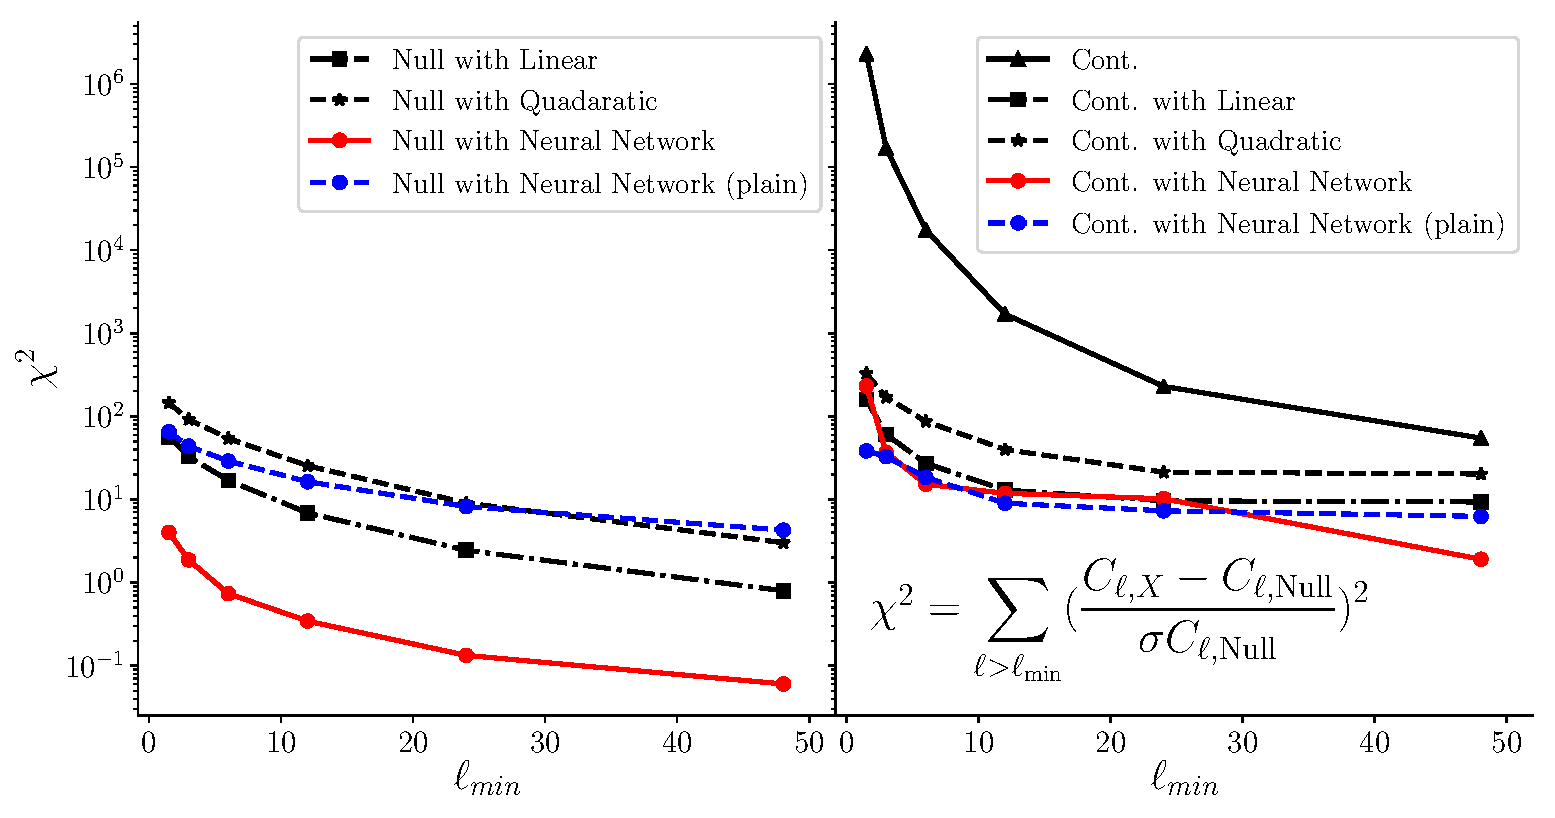
\includegraphics[width=0.7\textwidth]{mocks_deltacl_chi2.pdf}
\caption{To better quantify the bias introduced by each method, we evaluate the dependence of the bias on the lowest bin $\ell_{{\rm min}}$ that is included in the $\chi^{2}$ computation.}\label{fig:chi2clmock}
\end{figure*}

\begin{figure*}
\centering
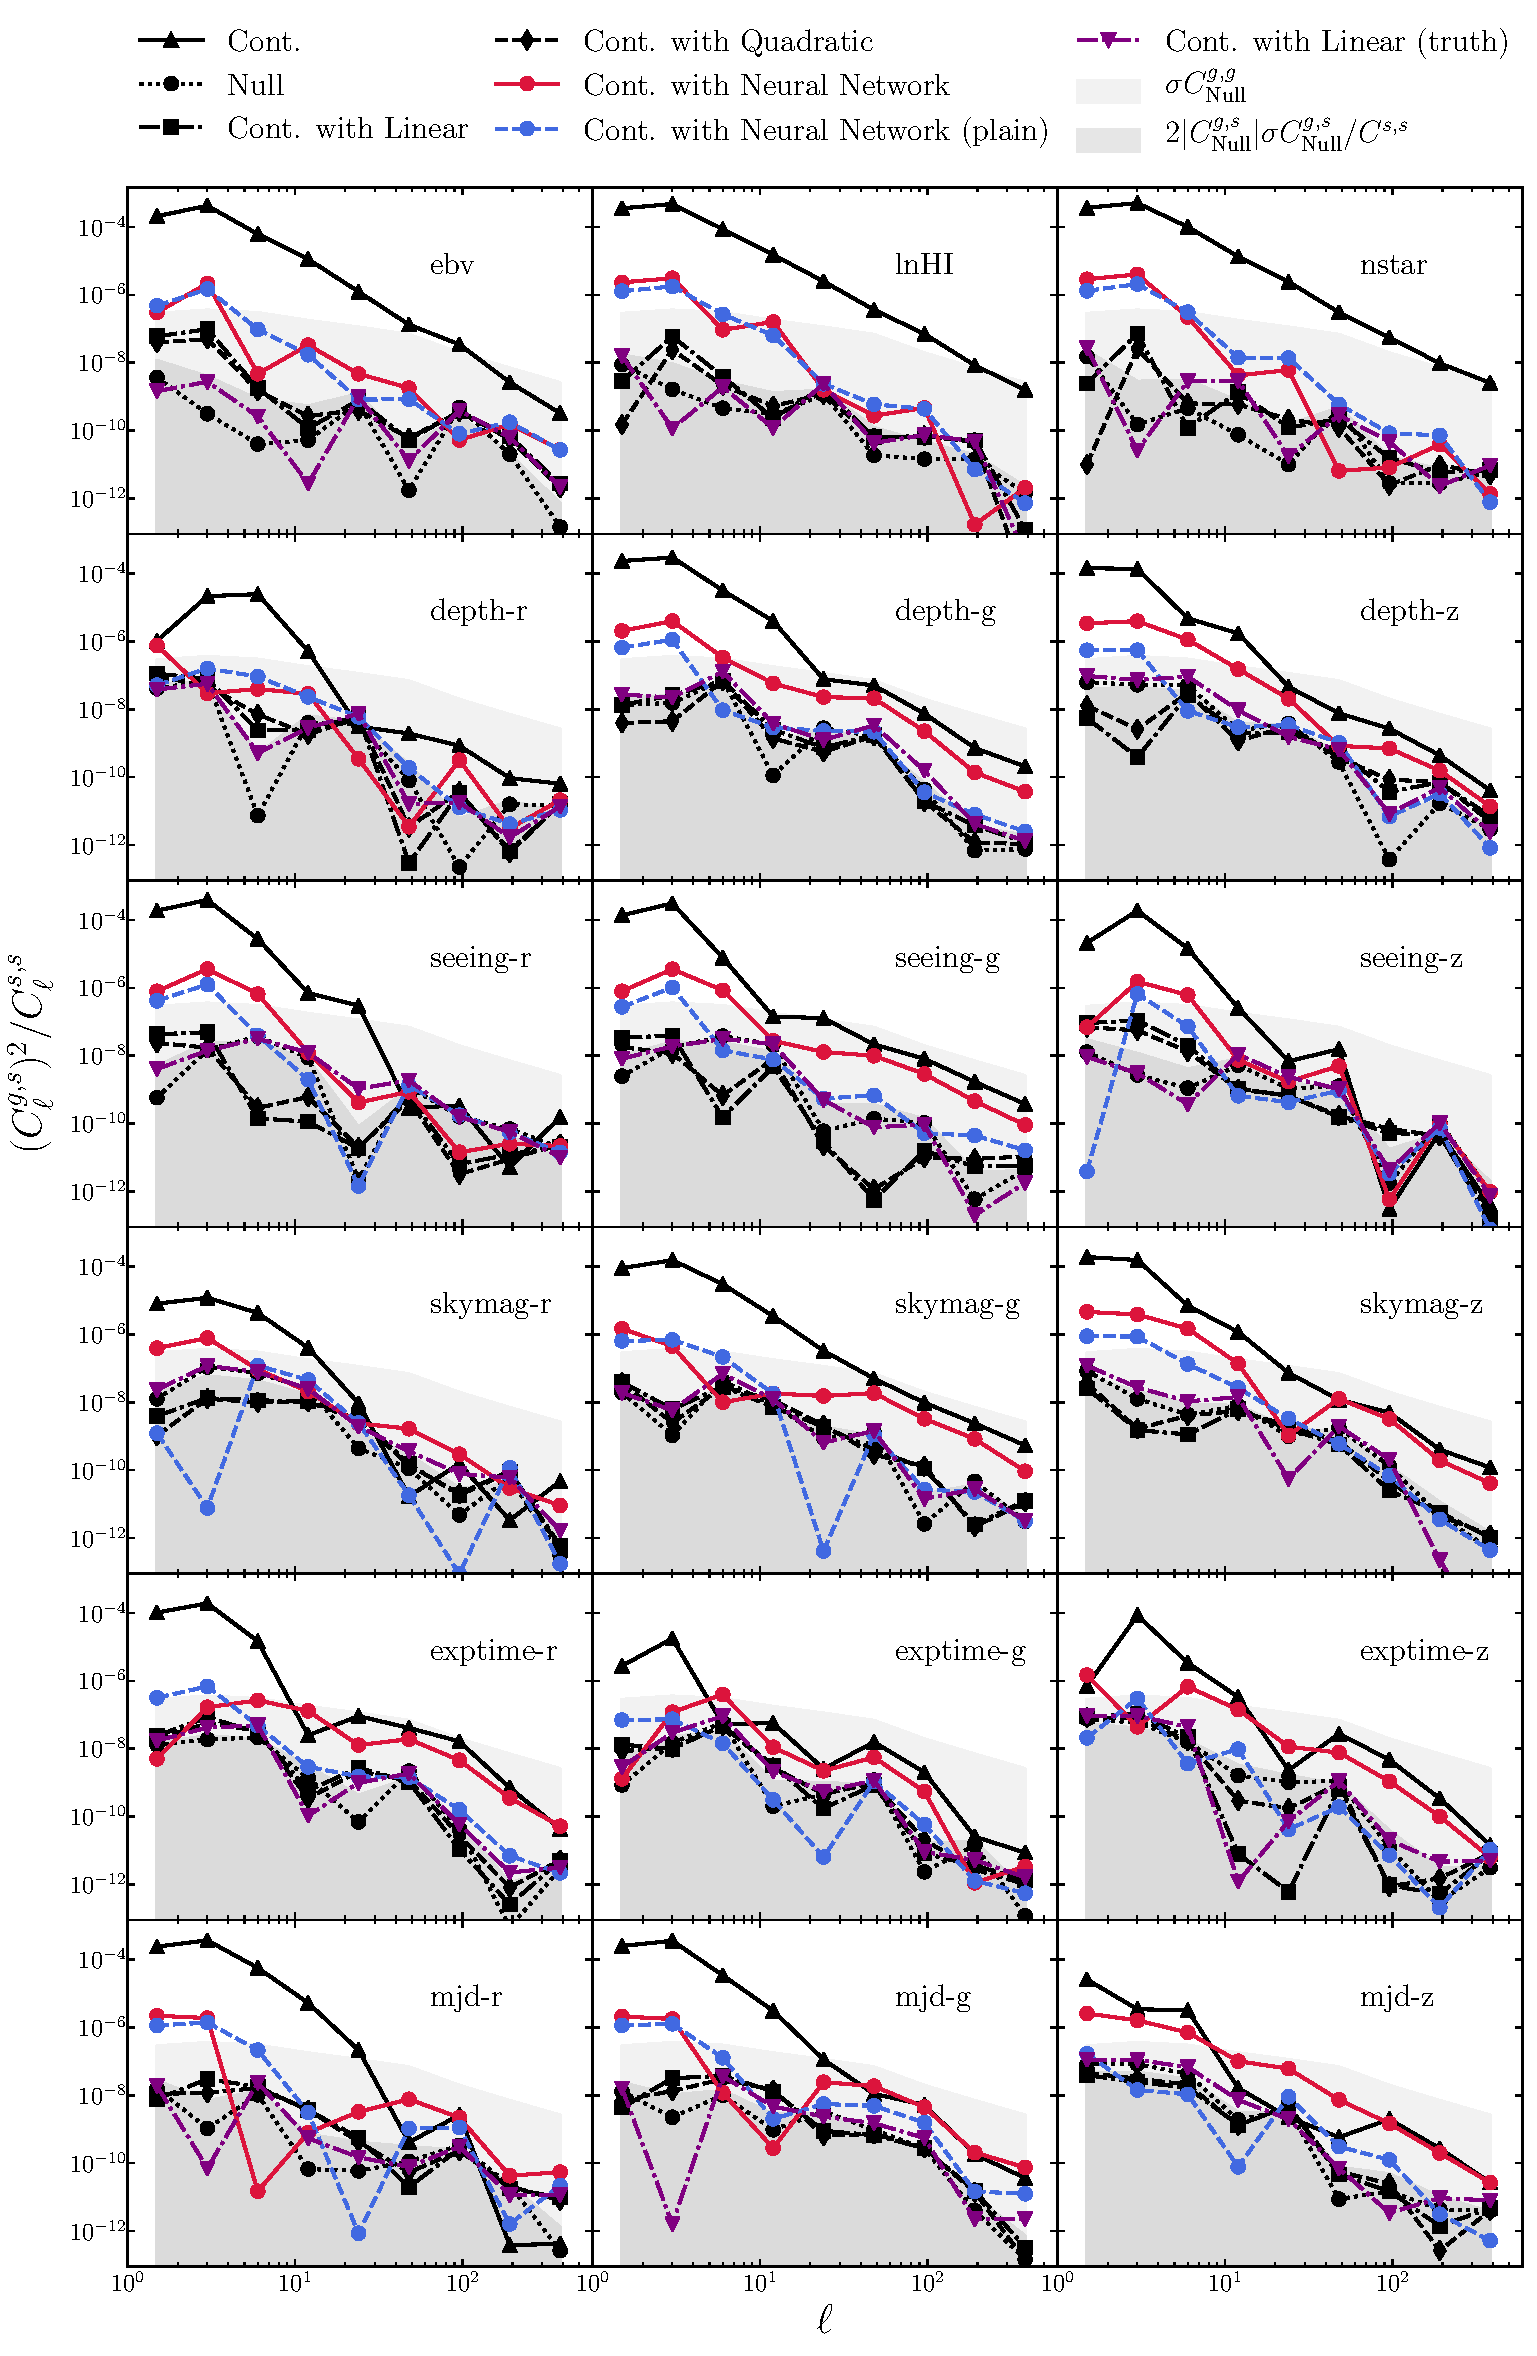
\includegraphics[width=0.8\textwidth]{cl-cross-mock_extra.pdf}
\caption{Cross power spectrum of the contaminated mock catalogs and the imaging attributes for different mitigation techniques. Our defaul neural network method with feature selection is shown in solid red while the performance without feature selection (`Neural Network (Plain)') is shown in dashed blue. The dark grey shaded region shows the 1$\sigma$ confidence region of the mean of the 100 mocks, and the light grey region shows the typical 1-$\sigma$ confidence region of one mock. The mitigation with the ground truth contamination model is shown with a purple dot-dashed curve as `cont. with linear (truth)'. \label{fig:clcrossmock}}
\end{figure*}
 
\begin{figure*}
\centering
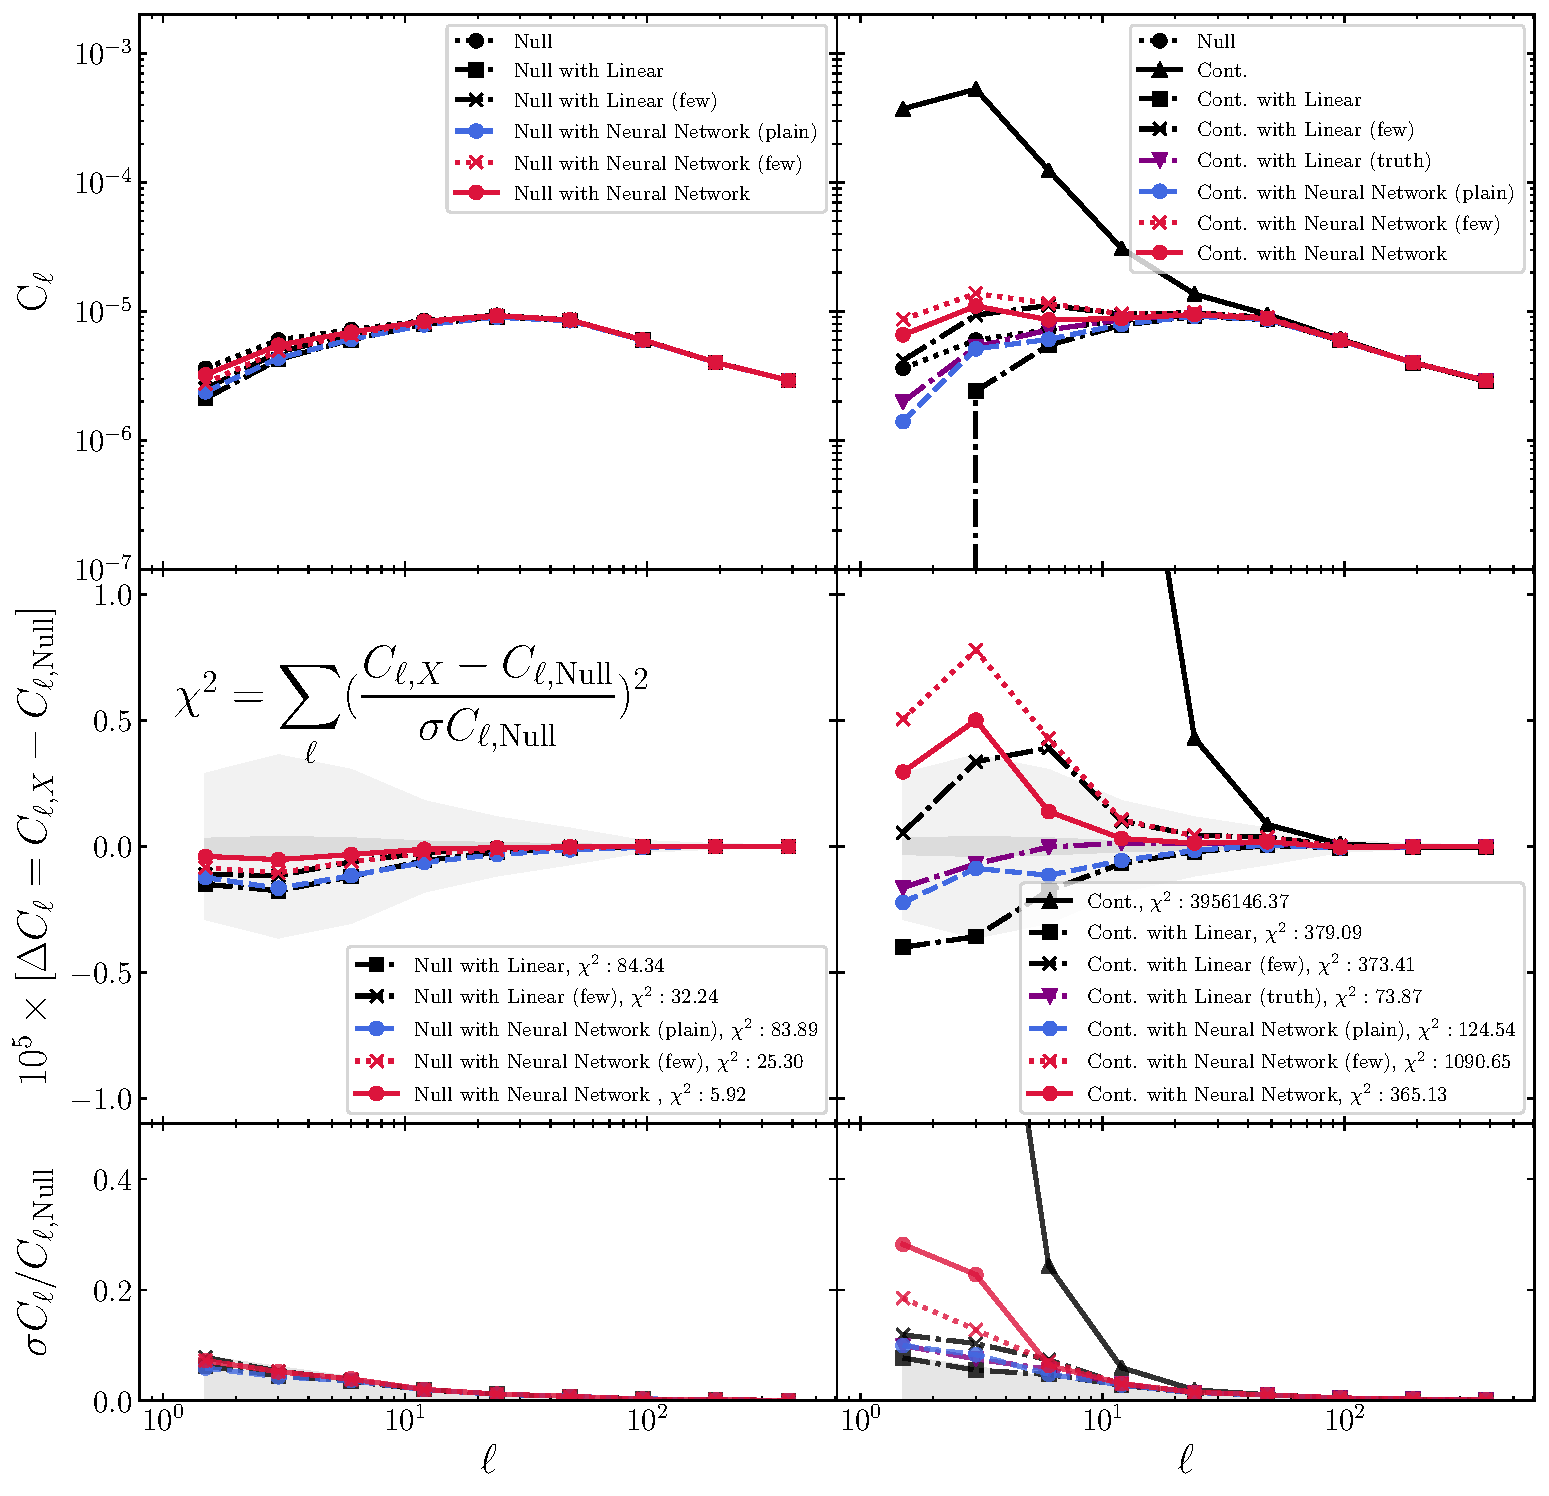
\includegraphics[width=0.7\textwidth]{mocks_deltacl_extra.pdf}
\caption{Same as Fig. \ref{fig:deltaclmock} showing the auto power spectrum results mitigated with the few imaging maps `few' (to demonstrate under-correction), neural network without the feature selection `plain', and the ground truth contamination model `truth'.}
\label{fig:mockdclextra}
\end{figure*}

\begin{figure*}
\centering
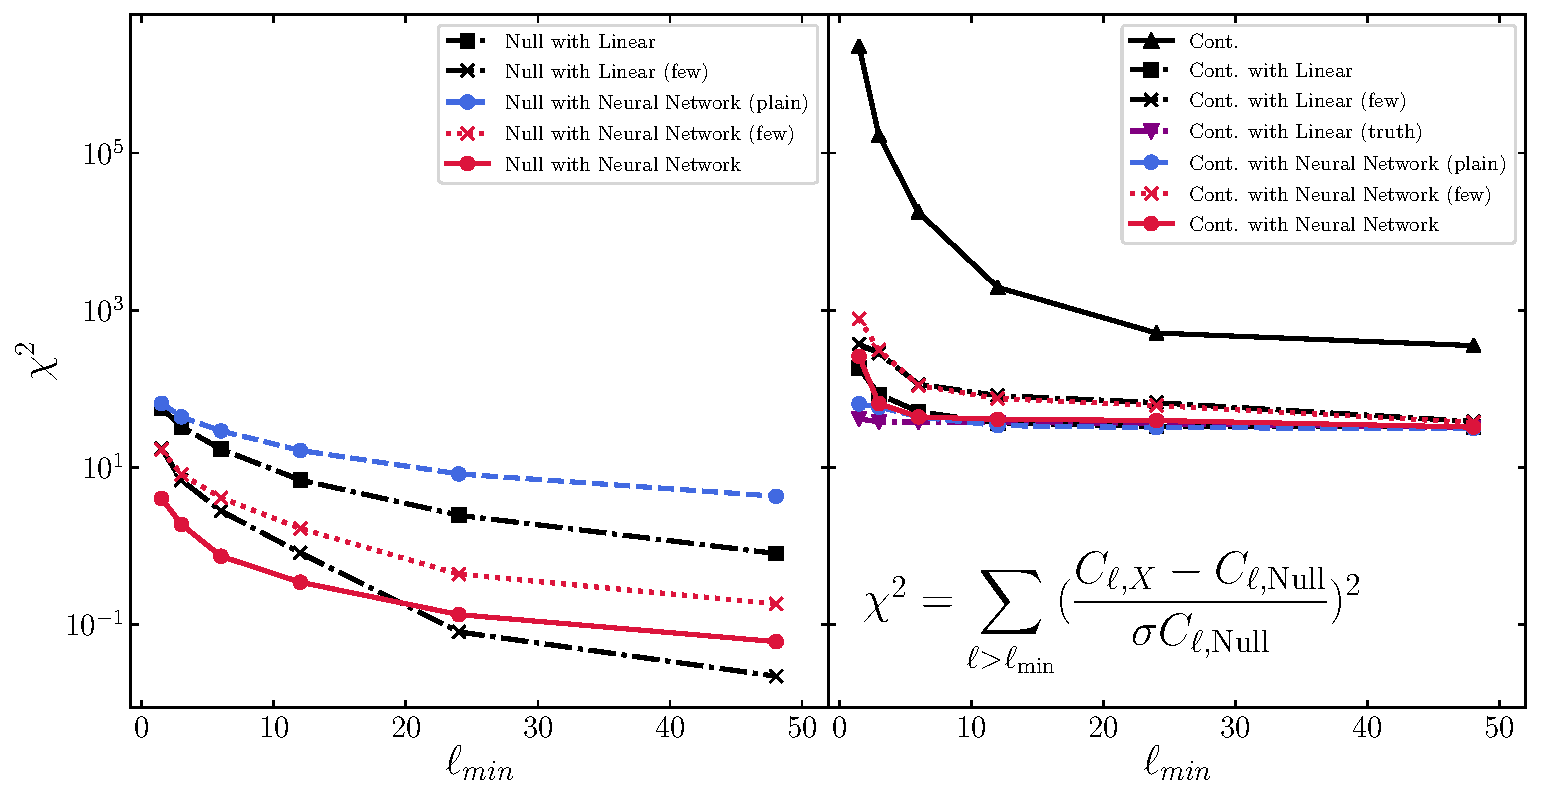
\includegraphics[width=0.7\textwidth]{mocks_deltacl_chi2_extra.pdf}
\caption{Same as Fig. \ref{fig:chi2clmock} showing the dependence of the bias after mitigation with the few imaging maps `few', neural network without the feature selection `plain', and the ground truth contamination model `truth'.}
\end{figure*}

\section{conclusion}\label{sec:conclusion}

In this paper, we have presented a rigorous application of an artificial neural network methodology to the mitigation of the observational systematics in galaxy clustering measurements of an eBOSS-like ELG sample selected from the DECaLS DR7 dataset (see \S~\ref{sec:data}). We have investigated the galaxy density dependency on 18 imaging attributes of the data (see Fig. \ref{fig:eboss_dr7}). We compare the performance of the neural network with that of the traditional, linear and quadractic multivariate regression methods. The key aspects of our neural network methodology are:\\

\textbullet ~the application of k-fold cross-validation, which implements the training-validation-test split to tune the hyper parameters by evaluating how well the trained network generalizes to the unseen,  validation data set and therefore to suppress overfitting when applied to the test set;

\textbullet ~the repeated split process until we cover the entire data footprint as test sets;

\textbullet ~the elimination of redundant imaging maps by the feature selection procedure to further reduce the overfitting problem and therefore protect the cosmological clustering signal.\\

We apply the output of our pipeline, i.e., the selection mask for the DECaLS DR7 footprint to the observed galaxy density field. Benchmark selection masks are also produced employing the linear and quadratic polynomial regression. Comparing statistical results before and after applying the selection masks, we find that:\\

\textbullet ~  Galactic foregrounds are the most dominant source of contamination in this imaging dataset (see Figs. \ref{fig:nnbar}, \ref{fig:clcross}, and \ref{fig:xicross}).

\textbullet ~    This contamination causes an excess clustering signal in the auto power spectrum and correlation function of the galaxy density field on large scales (see Fig. \ref{fig:clxi}).

\textbullet ~    All mitigation techniques e.g., the neural network method as well as the linear multivariate models using the linear and quadractic polynomial functions, are able to reduce the auto and cross clustering signals (see Figs. \ref{fig:xicross} and \ref{fig:clcross}); 

\textbullet ~ However, the neural network removes the excess clustering more effectively  in the auto power spectrum and correlation function of galaxies (see Fig. \ref{fig:clxi}), which leads to a better agreement between the measurement and the expected theoretical clustering based on the concordance flat $\Lambda$CDM universe.\\ 


The last result implies that our neural network method has a higher flexibility than both linear multivariate models we tested, and it is therefore capable of capturing the non-linear systematic effects in the observed galaxy density field.\\

We apply our methodology on two sets of 100 log-normal mock datasets with (`contaminated mocks') and without (`null mocks') imaging contamination  to evaluate how well the ground truth cosmological clustering can be reconstructed in both cases, and therefore to validate the systematic mitigation techniques. All mitigation techniques are applied in the same way we treat the real data. The key results of our mock test are as follows:\\

\textbullet ~ The feature selection procedure is able to identify most of the ten contamination input maps as important for the contaminated mocks while correctly identifying most of maps as redundant for the null mocks (see Fig. \ref{fig:mockablation}).

\textbullet ~    All three mitigation methods, i.e., the linear polynomial, quadratic polynomial, and neural network methods, perform equally well in terms of the residual bias in the presence of contamination. This is  expected since the contamination model is based on the linear polynomial model which all three methods are capable of reproducing. The neural network tends to slightly under-correct which is the outcome of the feature selection procedure. On the other hand, the linear and quadratic polynomial methods tend to slightly over-correct (see the right panel of Fig. \ref{fig:deltaclmock});

\textbullet ~    In the absence of contamination, the neural network is the most robust against regressing out the cosmological clustering. This is mainly due to the feature selection process that appropriately reduces the flexibility of the mitigation (see the left panel of Fig. \ref{fig:deltaclmock}). Based on this result, we implement the feature selection procedure for the DECaLS DR7 data.
    
\textbullet ~ All methods do not increase fractional variance during the mitigation process (see the bottom row of Fig. \ref{fig:deltaclmock}).\\


To conclude, our analyses illustrate that the neural network method we developed in this paper is a promising tool for the mitigation of the large-scale spurious clustering that is likely raised by the imaging systematics. Our method is more robust against regressing out the cosmological clustering than the traditional, linear multivariate regression methods. Such improvement will be particularly crucial for an accurate measurement of non-Gaussianity from the large-scale clustering of current eBOSS and upcoming DESI and the LSST surveys. Our method is computationally less intensive than other approaches such as the Monte Carlo injection of fake galaxies: analyzing the DECaLS DR7 data using our default neural network method requires less than six CPU hours. Application of our methodology on any imaging dataset would be straightforward. Our systematics mitigation methodology pipeline is publicly available at \url{https://github.com/mehdirezaie/SYSNet}.\\

% %Summary  

\section*{Acknowledgements}
M.R. and H.-J.S.~are supported by the U.S.~Department of Energy, Office of Science, Office of High Energy Physics under Award Number DE-SC0014329. This research used the Dark Energy Spectroscopic Instrument (DESI) allocation resources of the National Energy Research Scientific Computing Center (NERSC), a U.S. Department of Energy Office of Science User Facility operated under Contract No. DE-AC02-05CH11231. M.R. would like to thank Stephen Bailey, Anand Raichoor, Nick Hand, Yu Feng, Jeffrey Newman, Arnaud De-Mattia, Ted Kisner, Rollin Thomas, Marc Manera, Joel Brownstein, Dustin Lang, John Moustakas, Arjun Dey, and Patrick McDonald. 
%%%%%%%%%%%%%%%%%%%%%%%%%%%%%%%%%%%%%%%%%%%%%%%%%%

%%%%%%%%%%%%%%%%%%%% REFERENCES %%%%%%%%%%%%%%%%%%

% The best way to enter references is to use BibTeX:

\bibliographystyle{mnras}
\bibliography{refs} % if your bibtex file is called example.bib


% Alternatively you could enter them by hand, like this:
% This method is tedious and prone to error if you have lots of references
% \begin{thebibliography}{99}
% \bibitem[\protect\citeauthoryear{Author}{2012}]{Author2012}
% Author A.~N., 2013, Journal of Improbable Astronomy, 1, 1
% \bibitem[\protect\citeauthoryear{Others}{2013}]{Others2013}
% Others S., 2012, Journal of Interesting Stuff, 17, 198
% \end{thebibliography}

%%%%%%%%%%%%%%%%%%%%%%%%%%%%%%%%%%%%%%%%%%%%%%%%%%

%%%%%%%%%%%%%%%%% APPENDICES %%%%%%%%%%%%%%%%%%%%%

\newpage
\appendix
% \section{Feed Forward Neural Networks}



% % Don't change these lines
\bsp	% typesetting comment
\label{lastpage}

\end{document}
